%THIS IS THE MAIN FILE THAT TELLS LATEX WHICH FILES TO INCLUDE IN YOUR THESIS.

%THIS TEMPLATE PASSED DOWN FROM COURTNEY DRESSING
%EDITED SLIGHTLY AND UPLOADED TO OVERLEAF BY BEN COOK (bacook17@gmail.com)

% use "plain" for committee to read, or for printing single-spaced in general
\documentclass[plain]{hvdthesis}

% use "bound" for submitting to Harvard 
%\documentclass[bound]{hvdthesis}

% no more microfilm?
%\documentclass[microfilm]{hvdthesis}

% Put all required packages and setup in one file
%\usepackage{deluxetable}
%\usepackage{bibunits} %% bibunits.sty allows references at the end of each chapter

%\def\hsp{\def\baselinestretch{1.5}\normalsize} % intermediate spacing

\bibpunct{(}{)}{;}{a}{}{,}
\newcommand{\bmath}{\boldmath}
\usepackage{epstopdf}
\usepackage{epsfig}
\usepackage{aasmod}
\usepackage{amsmath}
\usepackage{amssymb}
\usepackage{rotating}
\usepackage{verbatim}
\usepackage{longtable}
\usepackage{lscape}
\usepackage{subfig}
\usepackage{float}
\usepackage{color}
\usepackage{fltpage}
\usepackage{url}
\usepackage{rotating}
\usepackage[innercaption]{sidecap}
\usepackage{pdfpages}
\usepackage{xspace}
\usepackage{wrapfig}
\setcounter{secnumdepth}{3}
%%--------
\usepackage{xargs}
\usepackage[colorinlistoftodos,prependcaption,textsize=tiny]{todonotes}
%These are custom definitions which you can change according to your taste.
\newcommandx{\info}[2][1=]{\todo[linecolor=violet,backgroundcolor=violet!25,bordercolor=violet,#1]{#2}}
\newcommandx{\change}[2][1=]{\todo[linecolor=blue,backgroundcolor=blue!25,bordercolor=blue,#1]{#2}}
\newcommandx{\unsure}[2][1=]{\todo[linecolor=OliveGreen,backgroundcolor=OliveGreen!25,bordercolor=OliveGreen,#1]{#2}}
\newcommandx{\improve}[2][1=]{\todo[linecolor=Plum,backgroundcolor=Plum!25,bordercolor=Plum,#1]{#2}}
\newcommandx{\thiswillnotshow}[2][1=]{\todo[disable,#1]{#2}}

%%---------




%this block is new from Greg S to accommodate change in 2013 format requiring page numbers be centered on every page
\usepackage{fancyhdr}
\pagestyle{fancy}
\fancyhf{}
\lhead{\it{\leftmark}}
\rhead{}
\chead{}
\cfoot{\thepage}
\lfoot{}
\rfoot{} 
\renewcommand{\headrulewidth}{0.0pt}

%\usepackage{apjfonts}

%% makes \subfloat command put (a), (b), ... labels at top of subfigure instead of bottom
\captionsetup[subfigure]{position=top,font=bf,captionskip=0pt,topadjust=0pt,farskip=0pt}

%\pagestyle{headings}
%\pagestyle{myheadings}
% could also have pagestyle{myheadings}
% problem w/ default headings is that they're
% a bit too wide for the page (the chapter titles are too long!)



% Put all your useful macros, shortcuts, and commands in one file
\newcommand{\ksmag}{\emph{Ks}~magnitudes }
\newcommand{\jmag}{\emph{J}~magnitudes }
\newcommand{\kpmags}{\emph{Kp}~magnitudes }
\newcommand{\kpmag}{\emph{Kp}~magnitude }
\newcommand{\teff}{\ensuremath{T_{\mathrm{eff}}}}                               
\newcommand{\logg}{\ensuremath{\log g}} 
\newcommand{\kepler}{{\em Kepler}\xspace}
\def\msun{{\rm\,M_\odot}}                                                       
\def\rsun{{\rm\,R_\odot}}        
\def\mearth{{\rm\,M_\oplus}}                                                
\def\rearth{{\rm\,R_\oplus}} 
\def\fearth{{\rm\,F_\oplus}} 
\def\lsun{{\rm\,L_\odot}}  
\newcommand{\hho}{H$_2$O}
\newcommand{\hh}{H$_2$}
\newcommand{\oo}{O$_2$}
\newcommand{\chhhh}{CH$_4$}
\newcommand{\mjup}{{\rm M}_{\rm Jup}}
\newcommand{\kms}{\rm km\ s^{-1}}
\newcommand{\mps}{\rm m\ s^{-1}}
\newcommand{\kelvin}{\rm K}
\newcommand{\degr}{\ensuremath{^\circ}}
\newcommand{\angstrom}{\rm \AA}
\newcommand{\oneday}{\rm day}
\newcommand{\days}{\rm days}
\newcommand{\hours}{\rm hours}
\newcommand{\meter}{\rm m}
\newcommand{\HST}{{\it HST}}
\newcommand{\hubble}{{\it HST}}
\newcommand{\spitzer}{{\it Spitzer}}
\newcommand{\zeroth}{$0^{\rm th}$}
\newcommand{\first}{$1^{st}$}
\newcommand{\second}{$2^{nd}$}
\newcommand{\third}{$3^{rd}$}
\newcommand{\fourth}{$4^{th}$}
\newcommand{\e}{${\rm e^{-}}$}
\newcommand{\persecond}{${\rm s^{-1}}$}
\newcommand{\perpixel}{${\rm pixel^{-1}}$}
\newcommand{\divideoot}{{\tt divide-oot}}
\newcommand{\modelramp}{{\tt model-ramp}}
\newcommand{\chisq}{$\chi^2$}
\newcommand{\calwf}{{\tt calwf3}}
\newcommand{\rp}{$R_{p}$}
\newcommand{\rs}{$R_{\star}$}
\newcommand{\flt}{{\tt flt}}
\definecolor{orange}{rgb}{.8,0.4,0}
\newcommand{\question}[1]{\sffamily {\em {\color{orange} [#1]}}\normalfont}
\newcommand{\todo}[1]{\sffamily {\em {\color{orange} #1}}\normalfont}
\newcommand{\edit}[1]{{#1}}
\newcommand{\mad}{\rm MAD}


\newcommand{\outline}[1]{
\todo{\begin{itemize}
#1 
\end{itemize}}}

\usepackage{natbib}
\bibliographystyle{aasjournal}
\usepackage{placeins} %Floatbarrier command
\PassOptionsToPackage{hyphens}{url}
\usepackage[colorlinks=true, allcolors=blue]{hyperref}
\usepackage{amsmath}
\usepackage{subfig}
\usepackage{graphicx}
\usepackage{siunitx}
\usepackage{comment}
\usepackage{svg}
\usepackage[normalem]{ulem}
\usepackage{romannum}
\usepackage{bm} %Bold math symbols
\usepackage{mathtools} %For dcases
\allowdisplaybreaks %To allow long equations to break pages.
\usepackage[T1]{fontenc} %To fix narrow underscores
\usepackage{textcomp} %For 'upquote' in listing
\usepackage{accsupp} %For non-copyable line numbers
\usepackage{nicefrac}
\usepackage{dsfont}
\usepackage{romannum}
\usepackage{xfrac}
\usepackage{ragged2e}

\usepackage{titlesec}
%\titleformat{\section}https://www.overleaf.com/project/60ee83c9e199e57c09f31d5b
%{\color{red}\normalfont\Large\bfseries}
%{\color{red}\thesection}{1em}{}

\newcommand{\sr}[1]{{\bf\color{red} [SR: #1]}}
\newcommand{\sroy}[1]{{\bf\color{magenta} #1}}
\newcommand{\suit}{{\it{SUIT}}}
\newcommand{\degree}{$^{\circ}$}
\newcommand{\isro}{{\it ISRO}}
\graphicspath{{./}{Figures/}}

\usepackage{enumitem}

\newlist{abbrv}{itemize}{1}
\setlist[abbrv,1]{label=,labelwidth=1in,align=parleft,itemsep=0.1\baselineskip,leftmargin=!}

\usepackage{tikz}
\usetikzlibrary{shapes.geometric, arrows}
\tikzstyle{io} = [rectangle, rounded corners, minimum width=3cm, minimum height=1cm,text centered, draw=black, text width=4cm, fill=cyan!30]
\tikzstyle{arrow} = [ultra thick,red,->,>=stealth]


\author{Soumya Roy | {\lbng \*s*eoumYo ray}}
\title{Solar Flares Across the Spectrum: Observations and Instrumentation}
\department{Jawaharlal Nehru University, New Delhi, India}
\subject{}
\month{July}
\year{2024}
\advisor{Prof. Durgesh Tripathi}

\begin{document}

% include the dissertation acceptance form
% \includepdf[pages={1}]{placeholder_dac.pdf}

\clearpage
\thispagestyle{empty}
\begin{center}
\vspace*{\fill}
Page left intentionally blank.
\vspace*{\fill}
\end{center}

\frontmatter

	%% Title page
\makecover
	%% Copyright
%\copyright

\newpage

\thispagestyle{plain}
{\centerline {\em "The first principle is that you must not fool yourself, }}
{\centerline {\em and you are the easiest person to fool."}}
{\rightline {\em {--} Richard P. Feynman}}

\newpage

\includepdf[pages={1,2,3}]{placeholder_dac.pdf}
\newpage
	%% Abstract
\abstract{
An ABSTRACT goes here.
}

%\input{abstract_short.tex}
	%% Table of Contents
{\singlespace
\tableofcontents
}
\newpage
\clearpage

	%% List of Figures
\addcontentsline{toc}{chapter}{List of Figures}
\listoffigures
\newpage
	%% List of Tables
\addcontentsline{toc}{chapter}{List of Tables}
\listoftables

\newpage
\clearpage

\thispagestyle{plain}
%\addcontentsline{toc}{chapter}{List of Publications}
\chaptermark{List of Publications}
\vskip 0.5cm
{\centerline {\Large \bf List of Publications}}
\vskip 0.5cm
\normalsize

\section*{Refereed Journal Publications}

%%%%%%%%%%%
\begin{itemize}
    \item ``Evolution of the Ratio of \ion{Mg}{2} Intensities during Solar Flares", {\bf Soumya Roy} and Durgesh Tripathi, 2024, ApJ, 964, 106, doi: \href{https://iopscience.iop.org/article/10.3847/1538-4357/ad2a46}{10.3847/1538-4357/ad2a46}\footnotemark[1]
    \item ``Near and Mid-ultraviolet Observations of X-6.3 Flare on 2024 February 22 Recorded by the Solar Ultraviolet Imaging Telescope on board Aditya-L1", {\bf Soumya Roy}, Durgesh, Tripathi, Sreejith, P, \& Ramaprakash, A. N., et. al., 2024, ApJL, 981, L19, doi:\href{https://iopscience.iop.org/article/10.3847/2041-8213/adb0be}{10.3847/2041-8213/adb0be}\footnotemark[1]
    \item ``Photometric Calibration \& Spectral Validation of the Solar Ultraviolet Imaging Telescope onboard Aditya-L1", Janmejoy Sarkar, {\bf Soumya Roy}, A. N. Ramaprakash,... 2024, J. Astron. Telesc. Instrum. Syst. 11(1), 014005 (2025), doi:\href{https://www.spiedigitallibrary.org/journals/Journal-of-Astronomical-Telescopes-Instruments-and-Systems/volume-11/issue-1/014005/Photometric-calibration-and-spectral-validation-of-the-Solar-Ultraviolet-Imaging/10.1117/1.JATIS.11.1.014005.short}{10.1117/1.JATIS.11.1.014005}\footnotemark[1]
    \item ``Science Filter Characterization of the Solar Ultraviolet Imaging Telescope (SUIT) on board Aditya-L1", Janmejoy Sarkar, Rushikesh Deogaonkar, Ravi Kesharwani, ... {\bf Soumya Roy},... 2024, Exp. Astron., 59, 3 (2025), doi: \href{https://doi.org/10.1007/s10686-024-09973-5}{10.1007/s10686-024-09973-5}
    \item ``Solar Ultraviolet Imaging Telescope on board Aditya-L1", Durgesh Tripathi, A. N. Ramaprakash, Sreejith P,... {\bf Soumya Roy},... 2025, Sol. Phys., 300, 30, \href{10.1007/s11207-025-02423-1}{10.1007/s11207-025-02423-1}\footnotemark[1]
    \item ``X-class flare on Dec 31, 2023, observed by the Solar Ultraviolet Imaging Telescope", {\bf Soumya Roy}, Durgesh Tripathi, Sreejith P, \& A. N. Ramaprakash, et. al., 2025, ApJL, 983, L6, \href{https://doi.org/10.3847/2041-8213/adc387}{10.3847/2041-8213/adc387}
    \item ``Test and Calibration of the Solar Ultraviolet
Imaging Telescope (SUIT) on board Aditya-L1", Janmejoy Sarkar, Nived V. N., {\bf Soumya Roy}, Rushikesh Deogaonkar et al., 2025, Accepted for publication in Sol. Phys.

\end{itemize}
%%%%%%%%%%%

\section*{Submitted Articles}

%%%%%%%%%%%
\begin{itemize}
    \item ``Evolution of thermal and cumulative non-thermal energy in solar flares", {\bf Soumya Roy}, Sophie Musset, Katharine K. Reeves, Durgesh Tripathi, Christopher S. Moore, 2024, Submitted to ApJ\footnotemark[1]{}\footnotetext{Part of this thesis}
    \item ``Forward Modeling Observations of the Solar Ultraviolet Imaging Telescope (SUIT) on board Aditya-L1", {\bf Soumya Roy}, L. S. Anusha, Durgesh Tripathi, et al. 2024, Submitted to ApJ\footnotemark[1]{}\footnotetext{Part of this thesis}
    %\item ``Critical Science Plan of the Solar Ultraviolet Imaging Telescope (SUIT) onboard Aditya-L1 mission", Durgesh Tripathi, A. N. Ramaprakash, ... {\bf Soumya Roy}, in Preparation
\end{itemize}
%%%%%%%%%%%

\section*{Technical Documents}

%%%%%%%%%%%
\begin{itemize}
    \item Roy, S., et al., "Solar Ultraviolet Imaging Telescope (SUIT) Handbook", ISRO Aditya-L1 mission
    \item Roy, S., et al., "Estimation of Effects of Space-craft Jitter on SUIT Imaging", ISRO Aditya-L1 mission\footnotemark[1]{}
\end{itemize}
%%%%%%%%%%%


\newpage
\clearpage

\thispagestyle{plain}
\addcontentsline{toc}{chapter}{List of Abbreviations}
%\chaptermark{List of Abbreviations}
\vskip 0.5cm
{\centerline {\Large \bf List of Abbreviations}}
\vskip 0.5cm
\normalsize

\begin{abbrv}

\item[AIA]  Atmospheric Imaging Assembly
\item[SDO]  Solar Dynamic Observatory
\item[EUV]  Extreme Ultra Violet
\item[HMI]  Helioseismic and Magnetic Imager 
\item[IRIS] Interface Region Imaging Spectrograph 
\item[EUI]  Extreme Ultraviolet Imager
\item[SUIT] Solar Ultraviolet Imaging Telescope
\item[STIX] the Spectrometer/Telescope for Imaging X-ray 
\item[ISRO] Indian Space Research Organisation 
\item[IMaX] Imaging Magnetograph eXperiment
\item[SuFI] SUNRISE Filter Imager
\item[QS]   Quite Sun
\item[CH]   Coronal Hole
\item[AR]   Active Region
\item[TR]   Transition Region
\item[DEM]  Differential Emission Measure
\item[EM]   Emission Measure
\item[LTE]  Local Thermodynamical Equilibrium 
\item[FoV]  Field of View
\item[RoI]  Region of Interest 
\item[LoS]  Line of Sight
\item[FWHM] Full Width Half Maxima
\item[MURaM] MPS/ University of Chicago Radiative MHD 

\end{abbrv}

\newpage
\clearpage
	%% Acknowledgments
%\noindent
The journey of a PhD is like a marathon. There are times when you feel like sprinting down the lane, full of energy, driven by small successes, getting stuck on something for a while, and finally finding that "eureka" moment. Other times, you feel out of breath, barely dragging your legs along, just trying to stand. I believe what matters most are the connections you make with people who push you and help you during those difficult moments—because without them, I wouldn't be here writing this acknowledgment!  

\noindent
First, I would like to thank Durgesh; this thesis would not have been possible without his guidance. He gave me enough freedom to explore whatever I wanted, offering valuable suggestions along the way but never giving "orders." More importantly, he carefully considered any differing viewpoints I raised from the first day. Without this freedom, I probably wouldn't be as proud of my growth over the past five years. Very few people get the opportunity to contribute to one of their country's first major observatory-class missions. I am especially grateful for the confidence he and Ram placed not only in me but also in several other young students while realizing SUIT. While I worked on the project for only five years, I also want to thank everyone who was part of it before me—without their hard work, I would not have been able to take over so easily.  

\noindent
Next, I would like to thank Kathy. Just like Durgesh, she also allowed me the freedom to explore the problems I was given, nudging me in the right direction whenever I got stuck. I also want to thank Chris. His enthusiasm in answering my questions and our discussions on various topics were invaluable. Working at CfA was a remarkable experience. I am grateful to Kathy, Durgesh, the Smithsonian Institution, and CfA for making this possible. Experiencing the life of a graduate student in two very different systems gave me insight into both the challenges and advantages of each. Beyond being a scientific opportunity, it was a profound lesson in becoming an independent person not just a "scientist". Leaving your country and loved ones after twenty-six years to live alone, work, cook, and function as an independent adult in a foreign country is not easy. But those one-and-a-half years helped me mature quickly.  

\noindent
Our memories of a place are deeply tied to the people and the experiences we share with them. I want to thank Tatiana and Chad specifically; I will forever cherish the fun we had in the chess club. Those library gatherings early on at CfA were something I looked forward to when I had not yet made many friends. Tatiana, you were a godsend! As someone who isn't very extroverted, you made it easy for me to open up to people at CfA. I also want to thank several people involved in the HSO-Connect project, with whom I had many fruitful academic and non-academic discussions: Sophie, Dana, Ritesh, Xiaoyan, Crisel, Dan, Sam, and Yeimy. Similarly, my time at IUCAA became equally memorable, thanks to many people—whether we were traveling, hiking, playing board games and football, cooking together, or organizing Diwali celebrations for two years in a row.  

\noindent
In the early days, I spent a lot of time with Sunil and Sorabh playing FIFA in my room or on the pantry TV. It was a relief to know I wasn’t the only one "wasting" time on "silly video games"! Tathagata, Suprovo, Sorabh, Sunil, Somak Da, Sourabh, Suraj, Dhruv, we spent so much time playing board games I had not even known existed. Ankush, Partha, Biku, Kavita, and Meenakshi, our cooking sessions and hangouts were respites I looked forward to. A special shout out to the football gang {—-} Sunil, Sorabh, Somak Da, Sayak, and Soumil. Thanks to you all, we managed to follow football regularly, despite our busy schedules.  

\noindent
I also thank the solar group and its wonderful members for both academic and non-academic discussions over the years: Nived, Vishal, Janmejoy, Megha, Sneha, Rushikesh, Rahul, Sreejith, Abhishek, Deepak, Sargam, and Avyarthana. Megha and Anirban felt like older siblings I could always approach when needed.  

\noindent
A special shout-out to Nived! Although we didn't spend much time together, I had more scientific discussions with you than anyone else. I respected your opinions so much that I started running every crazy idea by you first. Your constant presence in my scientific journey has been invaluable.  

\noindent
Special thanks to Lindsay Glesener. Many people never realize the impact they can have on others. During the 2023 SF AGU meeting, Chris took me with his group to Berkeley to see the FOXSI-4 assembled. At the time, I was at a low point, doubting my ability to succeed in academia and considering leaving after my PhD. Lindsay shared how, as a PhD student, she accidentally destroyed the CCD hours before the FOXSI-1 launch, delaying it. Despite that, she went on to become the PI of FOXSI-4. Her story rekindled my confidence. Lindsay, I may never tell you this in person, but however long I stay in academia, your story will remain a key source of inspiration.  

\noindent
I am deeply grateful to my professors at Presidency University, Kolkata {--} Suchetana and Ritaban for their support during my bachelor’s and master’s programs. Without them, I might not have pursued a PhD in astronomy.  

\noindent
This work would not have been possible without the support of my family and friends. I owe my career in physics to the enthusiasm and encouragement of my uncle, Maloy Kumar Roy, and my friend’s father, Ranjan Basak. My uncle Shyamal Kumar Ray has been a constant companion, whether watching football or movies together. Aloke Mitra has been a lifelong pillar of support. Sayan Chakraborty, who started as my teacher, gave me the coding skills that became invaluable during my PhD.  

\noindent
Finally, I want to thank my parents. They gave me the freedom to explore whatever I wanted from a very early age. After high school, they supported my decision to pursue a career in basic science, even when friends and relatives were skeptical.  

\noindent
This thesis would not have been possible without the open data policies of several instruments. I acknowledge the use of data from AIA, HMI, IRIS, XRT, STIX, Chandrayaan-2/XSM, Stereo-A, GOES/XRS, and GOES/SUVI. I also thank the SUIT and Pegasus servers at IUCAA for providing computational facilities.

\thispagestyle{plain}
\addcontentsline{toc}{chapter}{Acknowledgments}
\chaptermark{Acknowledgments}

\vskip 0.5cm
{\centerline {\Large \bf Acknowledgments}}
\vskip 0.5cm
\normalsize
\noindent
The journey of a PhD is like a marathon. There are times when you feel like sprinting down the lane, full of energy, driven by small successes, getting stuck on something for a while, and finally finding that "eureka" moment. Other times, you feel out of breath, barely dragging your legs along, just trying to stand. I believe what matters most are the connections you make with people who push you and help you during those difficult moments—because without them, I wouldn't be here writing this acknowledgment!  

\noindent
First, I would like to thank Durgesh; this thesis would not have been possible without his guidance. He gave me enough freedom to explore whatever I wanted, offering valuable suggestions along the way but never giving "orders." More importantly, he carefully considered any differing viewpoints I raised from the first day. Without this freedom, I probably wouldn't be as proud of my growth over the past five years. Very few people get the opportunity to contribute to one of their country's first major observatory-class missions. I am especially grateful for the confidence he and Ram placed not only in me but also in several other young students while realizing SUIT. While I worked on the project for only five years, I also want to thank everyone who was part of it before me—without their hard work, I would not have been able to take over so easily.  

\noindent
Next, I would like to thank Kathy. Just like Durgesh, she also allowed me the freedom to explore the problems I was given, nudging me in the right direction whenever I got stuck. I also want to thank Chris. His enthusiasm in answering my questions and our discussions on various topics were invaluable. Working at CfA was a remarkable experience. I am grateful to Kathy, Durgesh, the Smithsonian Institution, and CfA for making this possible. Experiencing the life of a graduate student in two very different systems gave me insight into both the challenges and advantages of each. Beyond being a scientific opportunity, it was a profound lesson in becoming an independent person not just a "scientist". Leaving your country and loved ones after twenty-six years to live alone, work, cook, and function as an independent adult in a foreign country is not easy. But those one-and-a-half years helped me mature quickly.  

\noindent
Our memories of a place are deeply tied to the people and the experiences we share with them. I want to thank Tatiana and Chad specifically; I will forever cherish the fun we had in the chess club. Those library gatherings early on at CfA were something I looked forward to when I had not yet made many friends. Tatiana, you were a godsend! As someone who isn't very extroverted, you made it easy for me to open up to people at CfA. I also want to thank several people involved in the HSO-Connect project, with whom I had many fruitful academic and non-academic discussions: Sophie, Dana, Ritesh, Xiaoyan, Crisel, Dan, Sam, and Yeimy. Similarly, my time at IUCAA became equally memorable, thanks to many people—whether we were traveling, hiking, playing board games and football, cooking together, or organizing Diwali celebrations for two years in a row.  

\noindent
In the early days, I spent a lot of time with Sunil and Sorabh playing FIFA in my room or on the pantry TV. It was a relief to know I wasn’t the only one "wasting" time on "silly video games"! Tathagata, Suprovo, Sorabh, Sunil, Somak Da, Sourabh, Suraj, Dhruv, we spent so much time playing board games I had not even known existed. Ankush, Partha, Biku, Kavita, and Meenakshi, our cooking sessions and hangouts were respites I looked forward to. A special shout out to the football gang {—-} Sunil, Sorabh, Somak Da, Sayak, and Soumil. Thanks to you all, we managed to follow football regularly, despite our busy schedules.  

\noindent
I also thank the solar group and its wonderful members for both academic and non-academic discussions over the years: Nived, Vishal, Janmejoy, Megha, Sneha, Rushikesh, Rahul, Sreejith, Abhishek, Deepak, Sargam, and Avyarthana. Megha and Anirban felt like older siblings I could always approach when needed.  

\noindent
A special shout-out to Nived! Although we didn't spend much time together, I had more scientific discussions with you than anyone else. I respected your opinions so much that I started running every crazy idea by you first. Your constant presence in my scientific journey has been invaluable.  

\noindent
Special thanks to Lindsay Glesener. Many people never realize the impact they can have on others. During the 2023 SF AGU meeting, Chris took me with his group to Berkeley to see the FOXSI-4 assembled. At the time, I was at a low point, doubting my ability to succeed in academia and considering leaving after my PhD. Lindsay shared how, as a PhD student, she accidentally destroyed the CCD hours before the FOXSI-1 launch, delaying it. Despite that, she went on to become the PI of FOXSI-4. Her story rekindled my confidence. Lindsay, I may never tell you this in person, but however long I stay in academia, your story will remain a key source of inspiration.  

\noindent
I am deeply grateful to my professors at Presidency University, Kolkata {--} Suchetana and Ritaban for their support during my bachelor’s and master’s programs. Without them, I might not have pursued a PhD in astronomy.  

\noindent
This work would not have been possible without the support of my family and friends. I owe my career in physics to the enthusiasm and encouragement of my uncle, Maloy Kumar Roy, and my friend’s father, Ranjan Basak. My uncle Shyamal Kumar Ray has been a constant companion, whether watching football or movies together. Aloke Mitra has been a lifelong pillar of support. Sayan Chakraborty, who started as my teacher, gave me the coding skills that became invaluable during my PhD.  

\noindent
Finally, I want to thank my parents. They gave me the freedom to explore whatever I wanted from a very early age. After high school, they supported my decision to pursue a career in basic science, even when friends and relatives were skeptical.  

\noindent
This thesis would not have been possible without the open data policies of several instruments. I acknowledge the use of data from AIA, HMI, IRIS, XRT, STIX, Chandrayaan-2/XSM, Stereo-A, GOES/XRS, and GOES/SUVI. I also thank the SUIT and Pegasus servers at IUCAA for providing computational facilities.



%\hfill -- RCH

\newpage
\clearpage
%	%% Dedication
%\input{dedication.tex}
\thispagestyle{plain}
\addcontentsline{toc}{chapter}{Dedication}

\vspace*{\fill}
{\centerline {\em Dedicated to everyone who pushed me one step at a time,}} 
{\centerline {\em every time I was about to give up!}}
{\centerline {\em And to my younger self, who was brave enough to embark on this journey...}}
%\vskip 1.5cm
%{\centerline {\em }}
\vspace*{\fill}

%\clearpage

\mainmatter
\pagestyle{fancy}


%% Uncomment the next four lines, plus the \begin{bibunit} and \end{bibunit} 
%% to use bibunits.  Read bibunits.dvi for more documentation
%\bibliographyunit[\chapter]
%\bibliographystyle*{apj}
%\bibliography*{apj-jour,planets}
%\bibliographyunit

\chapter[Introduction]{Introduction}\label{c:intro}
\input{./introduction/intro_2}
\clearpage
%
\chapter{Existing Solar Observations and Techniques: A bridge towards Solar Ultraviolet Imaging Telescope}\label{c:chap2}
\chaptermark{Solar Observatories and Analysis Techniques}
\input{./chapter2/chap2_2}
\clearpage
%
\chapter{Estimating thermal energy of two Solar Flares}\label{c:chap3}
\chaptermark{Solar flare energy}
%\begin{quote}
%{\em ~~~~~~~This thesis chapter originally appeared in the literature as} \\
%{authors,
%{\em journal reference info}}
%\end{quote}
\justifying

%%%%%%%%%%%%%%%%%%%%%%%%%%%%%%%%%%%%%%%%%%%%%%%%%%
\section{Introduction} \label{sec:intro}
%%%%%%%%%%%%%%%%%%%%%%%%%%%%%%%%%%%%%%%%%%%%%%%%%%

Solar flares are the largest magnetic events in our solar system. They are characterized by the eruptive release of magnetic energy, and manifest as localized transient heating of coronal plasma to temperatures over $\sim$ 10~MK. Flares are characterized by the full-disk integrated peak soft X-ray flux observed by the X-Ray Sensor onboard the {\it Geostationary Operational Environmental Satellites} \citep[{\it GOES}/XRS,][]{xrs} (``\textit{GOES class}''). The various components of the flare manifest in different wavelengths of the electromagnetic spectrum. The flare arcade and the fan exhibit the thermal plasma, while the majority of the non-thermal energy is from the foot points \citep{benz17}. The hot coronal plasma exhibited by flares is generally attributed to chromospheric evaporation, heated by the collisions of the flare-accelerated electrons in the impulsive phase \citep{fletcher11}. There is also strong evidence that the plasma might be directly heated in the corona in some cases \citep[e.g.][]{longcope11, reeves17}. 

There have been several works \citep{stosire07,emslie12,inglis14,warmuth16a,warmuth16b,ash17} that study the partition between the thermal and non-thermal energies in flares, which holds key insight into the relevant underlying physical processes in the flares. The results have been contradictory, and there is no consensus on whether non-thermal energetic electrons have enough energy to power the observed thermal energy component of smaller flares. These studies usually use peak thermal energy as a representative of the bulk thermal output of the flares. While these quantities are fair representation of the bulk thermal output of the flare, identifying subtle differences in the heating mechanisms at play at different stages of the flares requires a quantification of the thermal energy as a function of time.

There are several studies \citep{hilarie05,caspi10} that estimate thermal energy as a function of time. The thermal energy of the flares is defined as 
\begin{equation}
\mathrm{U_{Th}~\simeq~3n_{e}k_{B}TV}f,
\end{equation} \label{eq:t_eneg_1}
 where `$\mathrm{n_{e}}$' is the electron number density of the flaring plasma, `V' is the volume of the flaring plasma, `\textit{f}' is the volume filling factor, and `T' is the instantaneous temperature. One of the key challenges in characterizing the flares' thermal energy is determining the volume. 

\cite{li23} used $\frac{1}{e^{2}}$ contour of soft X-ray emitting region to identify the flare area `A', which was subsequently used to estimate the volume, $V\sim A^{\frac{3}{2}}$. \cite{zhang19} used a similar method, using intensity threshold on AIA 131~{\AA} observation, to estimate the flare area (A). \cite{hilarie05} used a similar method with {\it Reuven Ramaty High Energy Solar Spectroscopic Imager} \citep[{\it RHESSI},][]{rhessi} soft X-ray images to estimate the lower limit of the volume. They used {\it RHESSI} hard X-ray imaging to estimate the distance between two footpoints. Assuming a perfect ``arc-shaped" loop they calculated the upper estimate of the volume and concluded that the largest source of uncertainty in determining the thermal energy arises from the uncertainty in the filling factors.

\cite{hilarie05} also estimated the evolution of cumulative non-thermal energy injected by the electrons by assuming a thick-target model \citep{brown71} and fitting the {\it RHESSI} spectrum of the events. They fitted the {\it RHESSI} spectra in 25{--}35 keV bands to determine the non-thermal energies in time bins with significant emission above 25 keV. This process ensures a better accuracy for determining non-thermal energy by dividing the flare into short time intervals with large energy inputs, resulting in small thermal energy losses. They found that the non-thermal cumulative energy was larger than the thermal component of the flare for most of the duration of the flare. This is expected as radiative cooling significantly lower the temperature of the flare arcade as the flare evolves. They also deduced that during the early impulsive phase, the cumulative non-thermal energy could be lower than the thermal energy, depending on the estimates used for the flaring plasma volume. 

The filling factor `\textit{f}' quantifies the fraction of the apparent volume that is filled with the plasma of a specific temperature. It might also hold information about the geometric projection effects of the real volume into the apparent projected volume that is observed. Due to the highly multi-thermal nature of the flaring plasma and rapidly changing volume during the rise phase of the flare, it is challenging to define a filling factor that describes the plasma volume across the evolution of the flare. %Furthermore, most of the statistical studies so far, deals with bolometric or time averaged quantities near the peak of the flare.}
%This would indicate that direct heating possibly happens before or during the impulsive phase of flares.

\cite{caspi10} studied super hot flares from {\it RHESSI} observations, and used a 50\% intensity contour of cleaned {\it RHESSI} images to estimate the flare area, A. The volume $V=\frac{4}{3}\pi (A/\pi)^{3/2}$ was inferred from the area assuming spherical symmetry.  The two temperature components from the {\it RHESSI} spectral fit were assigned a volume V/2 each to estimate the total thermal energy. In all of these cases, the assumption of symmetrical expansion is useful because the thermal energy was estimated from a spectra obtained by integrating multiple pixels. There is no reliable way to address the spatially varying multi-thermal nature of the flaring plasma in these cases. 

In addition to the bulk thermal plasma in the flare loop, there are studies that suggested completely different heating mechanisms at play in specific flares. For example, \citet{longcope11} suggested a super hot plasma component in flares is directly heated in the corona in some large solar flares. Sustained temperatures in supra-arcade fans in flares have been hypothesized to be caused by supra-arcade down flows \citep[e.g.][]{reeves17}, suppression of conduction by turbulence \citep[e.g.][]{xie23} or global compression from reconnection inflows \citep[e.g.][]{reeves19}. These processes are distinctly different from chromospheric evaporation, which is characterized by the development of the hard X-ray foot-points and increasing intensity of soft X-ray and EUV-emitting plasma as the loops fill up.

%%%%######%%%%%%
\begin{figure}[ht!]
    \centering
    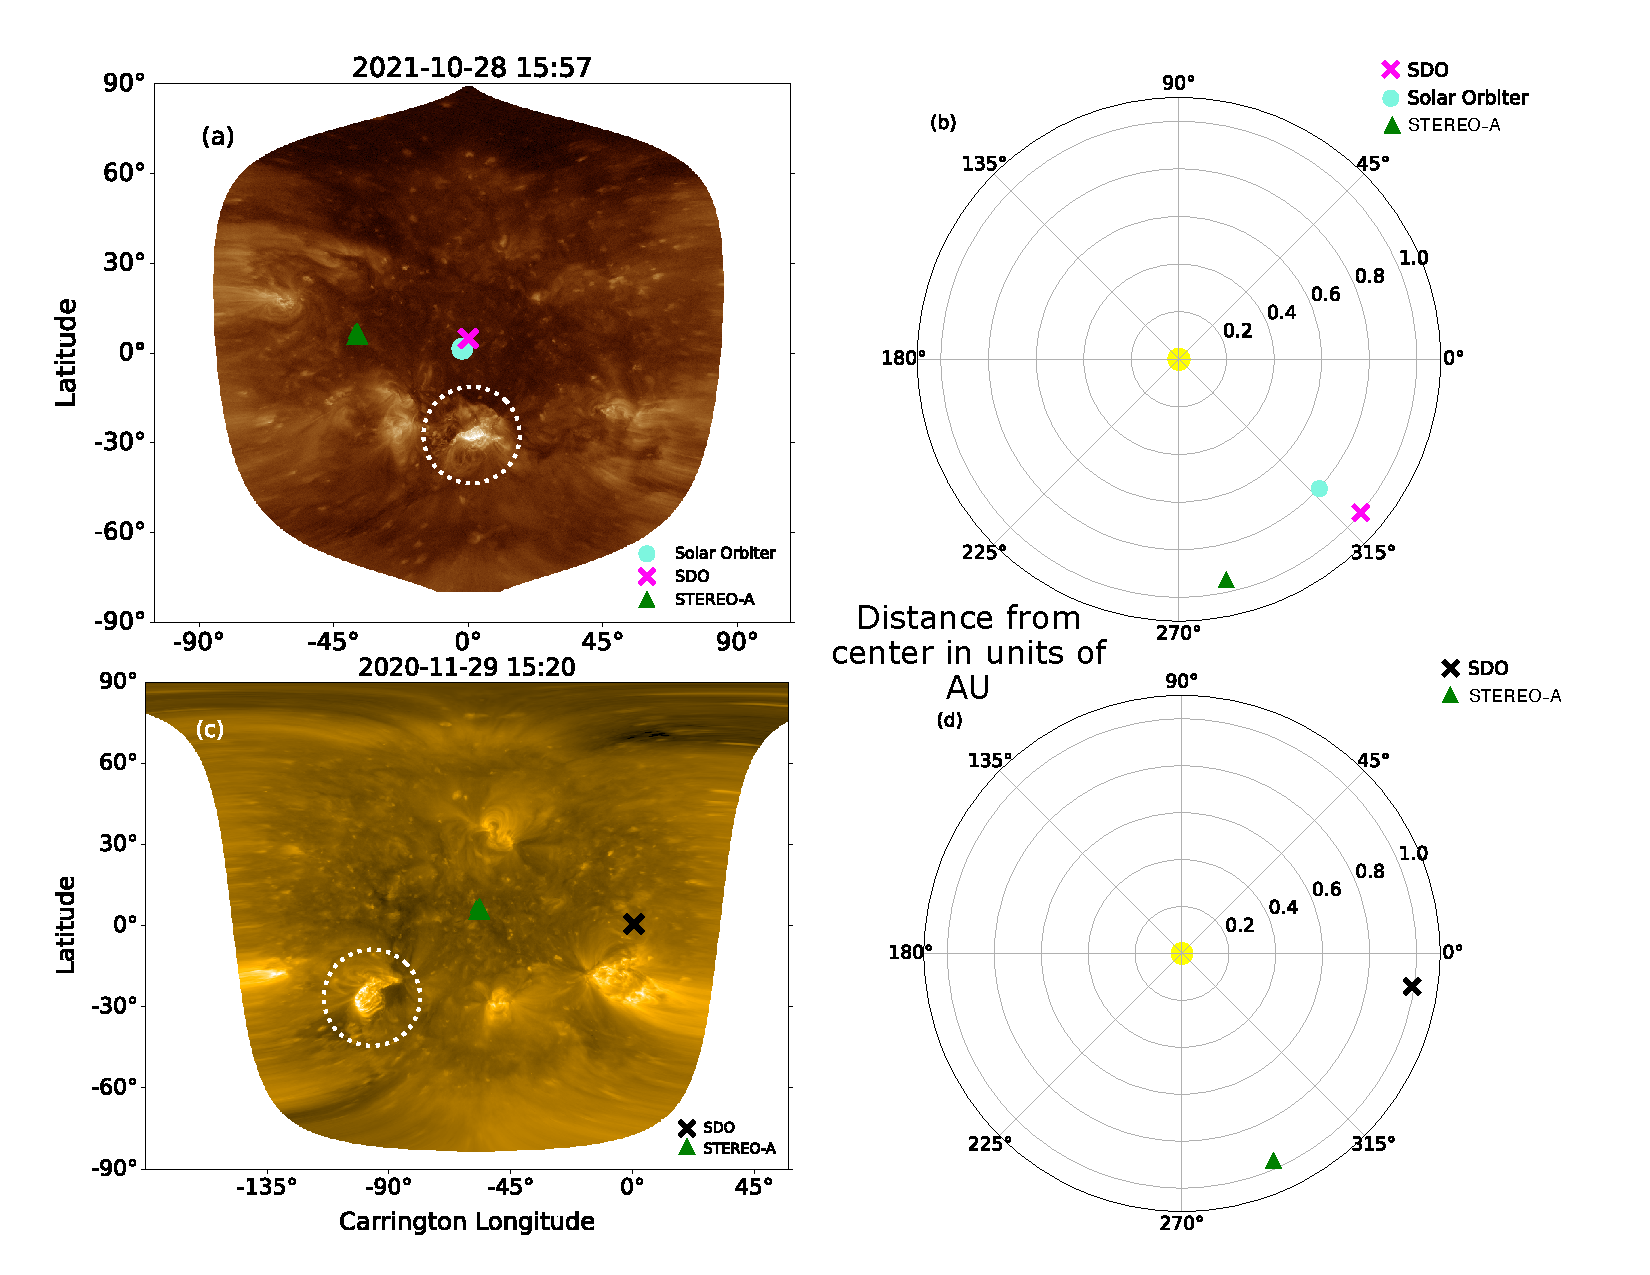
\includegraphics[trim={0cm 0.5cm 1.2cm 0.5cm},clip,width=\textwidth]{flare_pos.pdf}
    \caption[Position of various instruments during the flares.]{Position of various instruments during the flares. AIA 193~{\AA} observations during 2021 Oct 28 (panel a) and EUVI 171~{\AA} observation during 2020 Nov 29 (panel c) in Heliographic Stonyhurst (HGS) coordinates. The two flares studied here are enclosed by white dotted circle. The projected positions of {\it Solar Orbiter}, {\it SDO} and {\it STEREO-A} are marked as labelled. Positions of various spacecrafts projected onto the Heliocentric Inertial (HCI) frame for the for 2021 Oct 28 (panel c) and 2020 Nov 29 (panel d), as labelled.}
    \label{fig:sc_pos}
\end{figure}
%%%%######%%%%%%

Here we study the evolution of the thermal energy of two flares, \textit{viz.} M-class and X-class. We use existing tools and observations of the same region on the Sun from different vantages to estimate the volume of the flaring plasma more accurately. We show that a better estimate of the plasma volume affects the estimate of the thermal energy and has implications towards the energy budget of the flare. We also estimate the cumulative non-thermal energy deposited by the non-thermal electrons and compare it with our thermal energy estimates for the flare observed on 28 October, 2021. In \S\ref{sec:obs} we discuss the observations used in this {\bf chapter} and details of our analysis. We discuss our method for estimating the thermal energy in \S\ref{sec:therm}. In \S\ref{sec:los} and \S\ref{sec:non-therm}, we describe our method of volume estimation and cumulative non-thermal energy estimation, respectively. We discuss the results in \S\ref{res}.

%%%%%%
\begin{table}
    \centering
    \resizebox{\textwidth}{!}{%
    \begin{tabular}{||c|c|c||}
    \hline
    Instruments & Details & Flares\\
    \hline 
    \hline
      & 0.6 \arcsec/pix. Used&   \\
     {\it SDO}/AIA &  for estimating the thermal & 28 October, 2021 \\
     & properties. Temperature coverage & \& 29 November, 2020 \\
     & 5 $< log\ (T) <$ 7.5 & \\
         \hline
        & 2.5 \arcsec/pix. Has & \\
       & similar temp. response as AIA. & 28 October 2021 \\
      {\it GOES}/SUVI & Used for replacing saturated & \& 29 November, 2020 \\
       & AIA frames in DEM estimation & \\
       \hline 
        & 1 \arcsec/pix. Used simultaneously & \\
       & with AIA data in estimation of the thermal  & \\
     {\it Hindoe}/XRT  & properties. Temperature coverage  & 29 November, 2020 \\
       & 6.1 $< log\ (T) <$ 7.5, provides better & \\
       & constraints on the higher temp. end. & \\
       \hline 
       & 1.6 \arcsec/pix. Used & \\
       & for estimating the geometry & 28 October 2021  \\
     {\it STEREO-A}/EUVI   & of the arcade. 171 and 195 \AA & \& 29 November, 2020 \\
       & Observations are used with & \\
       & AIA 171 and 193 \AA. & \\
       \hline
        & X-ray imaging and spectroscopy in the  &   \\
       & 4-150 keV range. Soft X-ray imaging used & \\
      {\it SO}/STIX & for calculating the area of the flare. & 28 October 2021 \\
       &  Spectra used for constraining the thermal & \\
       & and non-thermal properties & \\
       \hline
       & Continuous full disk integrated soft X-ray light curve. & 28 October, 2021 \\
     {\it GOES}/XRS  & Used for estimating the bulk thermal & \& 29 November, 2020 \\
       & properties of the flare. & \\
       \hline
    \end{tabular}}
    \caption{List of the various instruments with their relevant specifications that were used for the analysis of the specific flares.}
    \label{tab:data}
\end{table}
%%%%%%


%%%%%%%%%%%%%%%%%%%%%%%%%%%%%%%%%%%%%%%%%%%%%%%%%%
\section{Observations and Data Analysis}\label{sec:obs}
%%%%%%%%%%%%%%%%%%%%%%%%%%%%%%%%%%%%%%%%%%%%%%%%%%

We study the two flares observed on 28 October, 2021 (X-class) and 29 November, 2020 (M-class) observed on the disk center and limb of the Sun, respectively, from the perspective of Atmospheric Imaging Assembly onboard the {\it Solar Dynamic Observatory} \citep[{\it SDO}/AIA,][]{sdo,aia} vantage point. For this study, we primarily use the observations from AIA, the Extreme Ultraviolet Imager onboard {\it Solar Terrestrial Relations Observatory-A} \citep[{\it STEREO-A}/EUVI,][]{stereo,euvi} and the Solar Ultraviolet Imager onboard {\it GOES} \citep[{\it GOES}/SUVI,][]{suvi}, along with imaging from the Spectrometer/Telescope for Imaging X-rays onboard {\it Solar Orbiter} \citep[{\it SO}/STIX,][]{so,stix,stix1}, the X-Ray Telescope onboard {\it Hinode} \citep[{\it Hinode}/XRT,][]{xrt} and the X-Ray Sensor onboard {\it GOES} \citep[{\it GOES}/XRS,][]{xrs}. For the relevant specification of the instruments used, refer to Table~\ref{tab:data}.

The positions of various spacecraft with respect to the flares' location on the solar disk is illustrated in Fig.~\ref{fig:sc_pos}. The AIA 193 {\AA} observation of the 2021 Oct 28 flare is projected to Heliographic Stonyhurst (HGS) coordinates in panel a, with {\it SDO} (magenta cross), {\it SO} (cyan circle) and {\it STEREO-A} (green triangle) positions marked with respect to the flare location in Fig.~\ref{fig:sc_pos}.a. The flare is marked with white dotted circle. The relative separation between the spacecrafts show the difference in the polar angle (vertical axis in Fig.~\ref{fig:sc_pos}.a) and azimuthal angle (horizontal axis in Fig.~\ref{fig:sc_pos}.a) introduced due to difference in vantages. The positions of the spacecrafts projected onto the Heliocentric Intertial (HCI) frame for the 2021 Oct 28 event is plotted in Fig.~\ref{fig:sc_pos}.b. The relative separation between the spacecrafts show the difference in azimuthal angle and the distance from the sun (distance from the center radially outwards in Fig.~\ref{fig:sc_pos}.b). We show the same for the 2021 Nov 29 flare in Fig.~\ref{fig:sc_pos}.c and d, with {\it STEREO-A}/EUVI 171 {\AA} emission projected to HGS and HCI coordinates.% {\bf We list out the various instruments used for the analysis of the two flares in Tab.~\ref{tab:data}.}

%%%%%%%%%%%%%%%%%%%%%%%%%%%%%%%%%%%%%%%%%%%%%%%%%%
\subsection{X flare on 28th October, 2021}\label{sec:x1-obs}
%%%%%%%%%%%%%%%%%%%%%%%%%%%%%%%%%%%%%%%%%%%%%%%%%%
%%--------------------------
\begin{figure}[ht!]
    %\hspace{-1cm}
    \centering
    \includegraphics[width=0.95\textwidth,trim={0.3cm 4cm 0cm 2cm},clip]{oct28_align_new.pdf}
    \caption[Observation of the X-class flare on October 28, 2021.]{X-class flare observed on October 28, 2021. Panel (a): the post eruption arcade as observed in AIA 193~{\AA}. Panel (b): Two ribbon of the flare observed in AIA 1600 {\AA}, overplotted with STIX soft X-ray contours of 4{--}15 keV (solid blue lines) and hard X-ray contours of 15{--}25 keV (dashed red lines). Panel (c): the emission measure map of the region integrated over the temperature range of 5$<\log\,T<$7.4. Panel (d): the obtained DEM weighted temperature.}
    \label{fig:flare}
\end{figure}
%%--------------------------
The X1 flare occurred on Oct 28, 2021 (SOL2021-10-28T15:35) near $\sim~[0\arcsec,-500\arcsec]$ solar coordinates as seen from AIA. The flare was observed by {\it SDO}/AIA, {\it STEREO-A}/EUVI, {\it GOES}/SUVI, and XRT, along with {\it GOES}/XRS and STIX observations. AIA observations provide imaging with 94, 131, 193, 171, 211 and 335 {\AA} passbands. SUVI provides imaging with similar wavelengths as AIA: 94, 131, 195, 171, 195 and 284 {\AA}, while {\it STEREO-A}/EUVI provides imaging in 171, 195, 284 {\AA} coronal passbands. The flare exhibits a standard two-ribbon structure, along with a ridge at the top of the rising flare arcade \citep{longcope22}. The ridge most prominently shows up in the AIA 193 {\AA} channel with contributions from \ion{Fe}{12} and \ion{Fe}{24}. %\cite{longcope22} showed that the ridge was mainly created by the hotter \ion{Fe}{24} line (T~$\simeq$~17~MK) and a height of the flare arcade, $h~\simeq~20~Mm$. We use this ridge to identify the loop-top in the AIA observation and calculate the height of the loop (see \S\ref{sec:los} for further details).

{\it SO}/STIX provides X-ray imaging and spectroscopy in the 4-150 keV range. Spectroscopic observations are provided with 32 pre-defined energy channels distributed in this energy range. STIX is an indirect imager measuring visibilities in the Fourier space, and images can be reconstructed from these visibilities with different algorithms. We use the MEM-GE algorithm \citep{massa20} to construct the STIX intensity maps.

In Figure.~\ref{fig:flare} (top row) we display the flare as observed with AIA~193 {\AA} (panel a) and 1600~{\AA} (panel b, inverted colors). These images reveal the two ribbon nature of the flare with post eruption arcades \cite[see e.g.][]{TriBC_2004}. We also overplot the STIX intensity contours (15:27:40 {--} 15:28:00 UT) in 4{--}15 keV (blue solid lines) and 15{--}25 keV (red dashed lines), on an AIA 1600 {\AA} image during the rise phase of the flare (see Fig.~\ref{fig:flare}.b). The STIX hard X-ray contour aligns with AIA 1600 {\AA} ribbons.


%%--------------------------
\begin{figure}[ht!]
\centering
    \includegraphics[trim={4.8cm 2.5cm 6cm 2.5cm},clip,width=0.8\textwidth]{nov_29_align.pdf}
    \caption[Observation of the M-class flare on November 29, 2020.]{M-class flare on Nov 29, 2020 as observed nearly simultaneously by AIA~{131 \AA} (panel a) and XRT Be-med filer (panel b) and the derived EM map (panel c) and DEM weighted temperature (panel d). The EM map is obtained by integrating over the temperature range of 5$<\log\,T<$7.4.}
    \label{fig:flare2}
\end{figure}
%%--------------------------

%%%%%%%%%%%%%%%%%%%%%%%%%%%%%%%%%%%%%%%%%%%%%%%%%%
\subsection{M flare on 29th November, 2020}\label{sec:m-obs}
%%%%%%%%%%%%%%%%%%%%%%%%%%%%%%%%%%%%%%%%%%%%%%%%%%

The M flare occurred on November 29, 2020, near $\sim [-950\arcsec,-430\arcsec]$ solar coordinates from the AIA perspective. In the AIA images, the footpoints were occulted behind the limb. The flare was also recorded by {\it STEREO-A}/EUVI, {\it GOES}/SUVI and {\it Hinode}/XRT. Along with these instruments, there were observations from {\it GOES}/XRS and {\it Fermi}/GBM. There were no observations from STIX for this event.

The flare exhibits a fan which is visible in the hot channels of AIA (131 and 193 {\AA}) and the XRT channels. Fig. \ref{fig:flare2}a shows an AIA 131 {\AA} image of the flare recorded during the decay phase. In Fig.~\ref{fig:flare2}b, we plot an XRT Be-med filter observation taken near simultaneous with the AIA image. For the M-class event, the {\it Fermi} observations were periodically eclipsed during the duration of the flare. We do not calculate the cumulative non-thermal energy for this event, as during the eclipses there is no reliable way to estimate the instantaneous non-thermal energy deposited. Hence, the estimation of cumulative non-thermal energy would not be a fair representation of the total non-thermal energy available.

%%%%%%%%%%%%%%%%%%%%%%%%%%%%%%%%%%%%%%%%%%%%%%%%%%%%
\subsection{Thermal Energy}\label{sec:therm}
%%%%%%%%%%%%%%%%%%%%%%%%%%%%%%%%%%%%%%%%%%%%%%%%%%%%

We estimate the thermal energy of the X-class event by calculating the differential emission measure (DEM) of the flaring region from the six AIA passbands including 94 {\AA} (\ion{Fe}{10} $\sim$1.1~MK, \ion{Fe}{18} $\sim$7.1~MK), 131 {\AA} (\ion{Fe}{8} $\sim$0.4~MK, \ion{Fe}{21} $\sim$11~MK), 171 {\AA} (\ion{Fe}{9} $\sim$0.6~MK), 193 {\AA} (\ion{Fe}{12} $\sim$1.6~MK, \ion{Fe}{24} $\sim$17~MK), 211 {\AA} (\ion{Fe}{14} $\sim$2~MK), 335 {\AA} (\ion{Fe}{16} $\sim$2.5~MK) \citep{o'dwyer10,O'Dwyer12}. Near the peak of the flare, several AIA frames are saturated in several instances and as such they cannot be used for the analysis. The SUVI temperature response is very similar to AIA~\citep{suvi}. Therefore, whenever necessary, the specific AIA frames can be replaced by those taken by SUVI for thermal energy estimates after co-aligning and co-registering  the two observations. Moreover, we also need to rescale the AIA temperature response functions to account for the binning of the AIA data to match the SUVI resolution. Note that since most of the XRT observations during the flare are saturated, we do not include them in our analysis of this flare.

For the M-class event, we estimate the thermal energy using AIA and XRT observations. Here, we bin the AIA observations to XRT pixel size, co-align, and calculate the DEMs. As described earlier, we rescale the AIA temperature response functions to account for the binning of the AIA data.

We use the regularized inversion method \citep{hannah&kontar12} to calculate the DEMs. The observed flux from the individual passbands can be written as,
%%%%%%%%%%%%%%%%%%%%%%%%
\begin{equation}
    F_{i}~=~\int~DEM_{c}(T)~R_{i}(T)~dT+\delta F_{i}
\end{equation}
%%%%%%%%%%%%%%%%%%%%%%%%
where $R_{i}$ is the temperature response of the passband `i', $\delta F_{i}$ is the error on the observed intensity for the passband `i' and $DEM_{c}(T)$ is the column differential emission measure (in units of $cm^{-5}K^{-1}$). The DEM inversion was performed for a temperature range $4.5~\le log(T)\le~8$.

With the inverted DEM, we calculate the column emission measure ($EM^{c}~\mathrm{in~units~of~cm^{-5}}$) and DEM-weighted temperature as:
%%%%%%%%%%%%%%%%%%%%%%%%%
\begin{equation}
    EM^{c}~=~\int_{T} DEM_{c}(T)~dT
\end{equation}
%%%%%%%%%%%%%%%%%%%%%%%%%
%%%%%%%%%%%%%%%%%%%%%%%%%
\begin{equation}
    \bar{T}~=~\frac{1}{EM^{c}}\int_{T} DEM_{c}(T)~T~dT
\end{equation}
%%%%%%%%%%%%%%%%%%%%%%%%%

The temperature range of the integration is set to $5 < \log\,T < 7.4$. We calculate and plot the emission measure (panel c in Figs.~\ref{fig:flare} \& \ref{fig:flare2}) and the DEM weighted temperature (panel d in Figs.~\ref{fig:flare} \& \ref{fig:flare2}) for all the pixels in the field of view (FOV) for both the flares.  

The main goal of calculating the DEM maps is to estimate the thermal energy (using Eqn.~\ref{eq:t_eneg_1}) arising from various parts of the flare arcade. As alluded to earlier, one of the most crucial quantity is to obtain the volume of the flaring plasm. For our analysis, the volume of the plasma along an individual pixel is given by $V_{j}~=~A\times~LOS_{j}$, where $LOS_{j}$ is the line of sight (LOS) for the j-th pixel in the FOV and $A$ is the physical area of a pixel.

We use the above expression for volume along with the emission measure and DEM weighted temperature estimated from the inverted DEM in Eqn.~\ref{eq:t_eneg_1} and sum over the pixels in the FOV to estimate the thermal energy arising from the FOV. This procedure gives us,
%%%%%%%%%%%%%%%%%%%%%%%%%%%%
\begin{equation}
    U_{Th}~=~\sum_{j}~\frac{3k_{B}A\sqrt{LOS_{j}}}{\sqrt{EM^{c}_{j}}}\int_{T}~DEM_{c}(T)_{j}T~dT
    \label{eq:t_eneg}
\end{equation}
%%%%%%%%%%%%%%%%%%%%%%%%%%%%
where $EM^{c}_{j}$ and $DEM_{c}(T)_{j}$ are the column emission measure and the column DEM in 5.0$<$$\log\,T$$<$7.4 for the j-th pixel in the FOV. We have used $n_{e}^{2}\times LOS~=EM^{c}$ and a filling factor $\textit{f}~=~1$. For the 2020 Nov 29 flare we mask the solar disk while calculating the DEMs and thermal energy. As evident from Eqn.~\ref{eq:t_eneg}, one of the major uncertainties in determining the emitting volume depends on determining the LOS for individual pixels in the FOV. 

%%%%%%%%%%%%%%%%%%%%%%%%%%%%%%%%%%%%%%%%
\subsubsection{Determining the LOS}\label{sec:los}
%%%%%%%%%%%%%%%%%%%%%%%%%%%%%%%%%%%%%%%%

We use co-temporal {\it STEREO-A} 171 {\AA}, 195 {\AA}, and AIA~171 {\AA}, 193 {\AA} images with \textit{scc\_measure.pro}, available in the \textit{sswidl}, to calculate the height of the loop. This routine allows us to select a point on the observation from one of the two vantages. The line of sight (LOS) through the same point is shown on the observation from the different vantage. The same point can be identified on the projected LOS by the user by identifying similar emission characteristics. The program determines the 3D coordinates of the point (heliographic latitude, longitude and radial distance). We carry out the same measurement at various positions along the loop top, to calculate the change in loop height across the arcade. With the different height measurements at various locations, we can calculate the volume of the flaring plasma under a semicircular assumption. We note that the height estimation using \textit{scc\_measure.pro} is limited by our identification of ``similar emission characteristics" between the two observations from AIA and {\it STEREO-A}. We choose multiple points on the top of the arcade, and calculate the height of the arcade at various locations tracing the looptop. The number of points we consider is not fixed and varies from frame to frame. After this, using the chosen points we interpolate to get the loop top from the AIA perspective, and the calculated height at these points gives us how the height of the loop top changes across the arcade. We assume a semi-circular loop geometry with the height of the loop top to calculate the LOS along every pixel within the flare arcade. It is worth reiterating that a majority of the uncertainty in determining the LoS would be arising from the identification of the loop top in two different vantages.

To infer the LoS along individual pixels in the FOV for both the flares, we use AIA and STEREO-A/EUI observations, recorded from two different vantage points, to calculate the height of {\bf both flare loops}. We show the STEREO-A/EUI 195~{\AA} and AIA 193~{\AA} observation for the Nov 29, 2020 flare in Fig.~\ref{fig:flare_orient2} panel b and a respectively. The blue cross marked in Fig.~\ref{fig:flare_orient2}.a is the LOS going into the page from AIA perspective. The blue line marked in Fig.~\ref{fig:flare_orient2}.b is the same LOS projected onto the STEREO-A perspective. The red crosses marked on the AIA 193~{\AA} loops mark the LoS going into the page, to infer the looptop from the AIA perspective. The red crosses marked on Fig.~\ref{fig:flare_orient2}.b EUVI 195~{\AA} observations marks the position of the looptop along the LoS from AIA perspective considered to find the looptop from EUVI perspective. In Fig.~\ref{fig:flare_orient2}.c we show the inferred LoS map for these two frames. The fan is assumed to have a constant LoS depth as mentioned earlier. For the loops we calculate the LoS assuming a semi-circular loop geometry with the height inferred from \textit{scc\_measure.pro}. The inferred LoS is lower near the loop top, and increases as we move closer the the foot points, exhibiting the variable LoS across the observation frame.

We display STEREO-A/EUVI and AIA-171 {\bf images} taken {\bf nearly} simultaneously in Fig.~\ref{fig:flare_orient} a~\&~b, respectively for the 28 Oct, 2021 event. The red and black cross on Fig.~\ref{fig:flare_orient}.a shows a point at the top of the flare arcade. The LOS goes into the page through that point from the {\it STEREO-A} vantage. The blue line in Fig.~\ref{fig:flare_orient}.b shows the LOS through the point in Fig.~\ref{fig:flare_orient} a projected to {\it SDO}/AIA point of view. This demonstrates the geometric effect of observing from different vantage points. In Fig.~\ref{fig:flare_orient}.c we show the inferred LoS map from the AIA perspective. 

%We show the same in Fig.~\ref{fig:flare_orient2} for the Nov 29, 2020 flare. The blue cross marked in Fig.~\ref{fig:flare_orient2}.a is the LOS going into the page from AIA perspective. The blue line marked in Fig.~\ref{fig:flare_orient2}.b is the same LOS projected onto the STEREO-A perspective. The red crosses marked on the AIA 193~{\AA} loops mark the LoS going into the page, to infer the looptop from the AIA perspective. The red crosses marked on Fig.~\ref{fig:flare_orient2}.b EUVI 195~{\AA} observations marks the position of the looptop along the LoS from AIA perspective considered to find the looptop from EUVI perspective. Distances on the observation from two different vantages would be projected by the differences in the polar and the azimuthal angle between the two vantages. 

%Fig.~\ref{fig:flare_orient_2}.a shows the projection effect of a semicircular loop between AIA and STEREO-A LOS. Depending on the orientation of the loops, the projection along the polar and azimuthal angle projects the length of the loop and the height of the loop. The height at various {\bf positions} of the flare arcade is marked in Fig.~\ref{fig:flare_orient2}.a. We assume a semi-circular loop geometry with the height of the loop top to calculate the LOS along every pixel within the flare arcade.

%%--------------
\begin{figure*}[!h]
    \centering
    \includegraphics[width=\textwidth, trim={1cm 0cm 1cm 3cm}, clip]{paper_plot_los.pdf}
    \caption[LoS triangulation for the Nov 29th, 2020 flare]{(a) SDO/AIA 193 {\AA} observation of the Nov 29 flare in the decay phase. The red and blue crosses marks various points on the top of the arcade used to trace the looptop. The LOS goes into the page from AIA perspective. (b) {\it STEREO-A}/EUVI 195 {\AA} observation around same time. The blue solid line is the LOS from AIA perspective in panel (a) projected onto {\it STEREO-A} perspective. The red crosses mark the other red crosses from AIA perspective marked on the looptop visible from Stereo-A perspective. The line of sight of the region is shown in panel (c). The LoS is higher near the base of the loops and lower near the looptop. The fan is assumed to be constant LoS.}
    \label{fig:flare_orient2}
\end{figure*}
%%--------------

%%--------------
\begin{figure*}
    \centering
    \includegraphics[width=\textwidth, trim={1cm 0cm 1cm 3cm}, clip]{paper_plot_los_2.pdf}
    \caption[LoS triangulation for the Oct 28th, 2021 flare]{(a) {\it STEREO-A}/EUVI 171 {\AA} observation of the {\bf Oct 28} flare arcade in the decay phase. The red and black cross marks a point on the top of the arcade. The line of sight (LOS) goes into the page through that point. (b) SDO/AIA 171 {\AA} observation of the flare arcade. The blue line marks the LOS through the arcade from the STEREO-A perspective projected to the AIA perspective. The red crosses mark the other red crosses from Stereo-A perspective marked on the loop top visible from AIA perspective. The line of sight of the region is shown in panel (c).}
    \label{fig:flare_orient}
\end{figure*}
%%--------------

The extent of the flare arcade is calculated by selecting pixels from the FOV which are located within an emission measure contour of 5\% of the peak emission measure value. It is possible to calculate the extent of the flare arcade from the intensity observed from any of the {\it SDO}/AIA or STIX imaging (for further details about the STIX imaging procedure, please refer to \cite{massa20}). However, due to the highly multi-thermal nature of the plasma, this procedure might be prone to missing significant portions of the flare arcade. The emission measure inferred from the DEM, on the other hand, reflects the density of the plasma in the entirety of the concerned temperature range of $5<\log\,(T)<7.4$. Therefore we find that, a 5\% contour of peak emission measure gives a better estimate of the extent of flare arcade. Outside of the flare arcade, we assume a LOS~$\sim$~2 Mm (the average thickness of chromosphere). 

%%%%%%%%%%%%%%%%%%%%%%%%%%%%%%%%%%%%%%%%%%%%%%%%%%%%
\subsection{Energy in the non-thermal electrons}\label{sec:non-therm}
%%%%%%%%%%%%%%%%%%%%%%%%%%%%%%%%%%%%%%%%%%%%%%%%%%%%

We estimate the energy in the non-thermal electrons for the 2021 Oct 28 X-class event by fitting the STIX spectra. In Fig.~\ref{fig:stix_an}.a, we plot the STIX light curve of the event in 4 to 10 keV (solid blue line), 10 to 15 keV (solid orange line), 15 to 25 keV (solid green line) and 25 to 50 keV (solid red line). The attenuator kicked in around $\sim$ 15:28 UT, which drastically cuts down the intensity to avoid saturation. The hard X-ray peak is visible in the 25 to 50 keV (solid blue line) at $\sim$ 15:28 UT. The soft X-ray peak is visible within the attenuated flux in 6 to 12 keV (solid magenta line) at $\sim$ 15:30 UT.

%%--------------
\begin{figure*}
    \centering
    \includegraphics[trim={0cm 3cm 1.3cm 3cm}, clip, width=\textwidth]{Figures/oct_28_lc_3.pdf}
    \caption[STIX light curve and spectra fit for the 2021 Oct 28 flare]{Panel a: STIX light curve of the 2021 Oct 28 X-class event in different energy bands as labeled. Panel b: STIX spectra integrated between 15:27:00{--}15:27:10~UT during impulsive phase, fitted with `\textit{thcik2}' (solid yellow), `\textit{vth}' (solid green) and the complete fit function `\textit{vth+thick2}' (solid red line). The panel (c) shows the normalized residuals of the fit.}
    \label{fig:stix_an}
    \end{figure*}
%%--------------

We closely follow the method described in \cite{emslie12} to estimate the energy deposited by the non-thermal electrons. We fit the STIX spectra of the event averaged over several time bins during the evolution of the flare with `\textit{vth}' and `\textit{thick2}' functions available in the `\textit{OSPEX}' X-ray spectra fitting package in {\it sswidl}. We show a reference fit to the spectra obtained over a time bin $\sim$ 15:27:00-15:27:10 UT in Fig.~\ref{fig:stix_an} panel (b) with `\textit{vth}' (solid green) and `\textit{thick2}' (solid yellow). The function `\textit{vth}' is a two-component thermal function. The parameters are the emission measure and temperature of the two thermal components and the relative abundances of Iron/Nickel, Calcium, Sulfur and Silicon with respect to the coronal abundances of CHIANTI \citep{chianti1,chianti}. The `\textit{thick2}' assumes the non-thermal component to be bremsstrahlung from energetic electrons with an injected spectrum $F_{0}(E_{0})~(e^{-}s^{-1}cm^{-2}keV^{-1})$ in the form of a broken power law:

%%--------
\begin{equation}
    F_{0}(E_{0})=A
    \begin{cases}
        0, & E_{0}<E_{min} \\
        E_{0}^{-\delta_{1}}, & E_{min} \le E_{0} < E_{b} \\
        E_{0}^{-\delta_{2}}E_{b}^{\delta_{2}-\delta_{1}}, & E_{b} \le E_{0} < E_{max} \\
        0, & E_{max} \le E_{0}
    \end{cases}
\end{equation}
%%--------

The parameters of this model spectrum, e.g., the normalization parameter A, the low- and high-energy cutoffs $E_{min}$ and $E_{max}$, break energy $E_{b}$, the power law indices $\delta_{1}$ and $\delta_{2}$ below and above the break are constrained by the fitting. We only fix the high energy cutoff at $3.2\times 10^{4}$ keV for every fit. The high energy cutoff is fixed much higher than our concerned energy range ($\sim$ O($10^{1}$ keV)), and we can safely assume that it has a negligible effect on fitting the X-ray spectra \citep{emslie12}. {\bf While this serves our purpose of quantifying the bulk non-thermal energy as a function of time, there can be finer details of the physical parameters from the "cold thick target" model that can pose non-physical conditions during the early rise phase of the flares. This can also have noticeable effect on the total thermal energy budget of the flare. To mitigate this several modifications of the cold thick target model have been proposed, e.g., local re-acceleration of electrons and ions \citep{brown09}, warm thick target model \citep{kontar15, kontar19} and injection of kappa distributed electrons instead of power law \citep{kasparova09, bataglia15, effenberger17}. We describe the physical origin of some of these models and their effects on the inferred injected electron spectra in Appendix~\ref{c:a2}. We also fit two of the modified models to the same spectra and compare the differences that arise due to that.}

The `\textit{OSPEX}' fitting is done by a forward fitting procedure. The parameters of the functions `\textit{vth}' and `\textit{thick2}' are varied to generate a photon spectrum, which is folded through the detector response matrix to produce a count rate spectrum. This count rate spectrum is used to constrain the parameters of the functions through an iterative procedure by minimizing the $\chi^{2}$ between the calculated and measured count rate spectrum. We provide the fitted temperature and the EM of the hotter thermal component in Tab.~\ref{tab:tab1} during various phases of the flare. The temperatures listed in Tab.~\ref{tab:tab1} is lower than the upper limit of the temperature range used ($5.0 \geq \log\,T \leq 7.4)$ %($log(T_{max})~=~7.4$ and $log(T_{min})~=~5$) 
to calculate the EM and DEM weighted temperature in \S\ref{sec:therm}.

%%%%%%%%%%%
\begin{table}
    \centering
    \resizebox{0.9\textwidth}{!}{%
    \begin{tabular}{|cl||c|c|}
    \hline
         &  & log(T) & EM \\ 
         & \hspace{-1cm}Time (UT) & of thermal component & ($cm^{-3}$) \\
    \hline
        Impulsive phase & \hspace{1.5cm}15:26 & 7.098 & $10^{48}$\\
        HXR peak & $\sim$ 15:27:20 - 15:28:20 & 7.19 & $3\times 10^{48}$\\
        Right after SXR peak & $\sim$ 15:35:39 - 15:36:34 & 6.88 & $4.1\times 10^{49}$\\
        Into the decay phase & \hspace{0.9cm}14:48:20 & 6.5 & $2\times 10^{49}$\\
        \hline
    \end{tabular}}
    \caption{Fitted temperature of the hotter component of the thermal plasma during various stages of the flare.}
    \label{tab:tab1}
\end{table}
%%%%%%%%%%%

The non-thermal energy in the electrons ($U_{e}$) at any instant $t=t'$ can be estimated by integrating the best-fit electron energy spectrum via: $$U_{e}(t=t')~=~\Delta t\int_{E_{min}}^{E_{max}}~F_{0}(E_{0})(t=t')dE_{0}$$ where the electron energy distribution in constrained by fitting the count spectra for the time interval $t'-\Delta t/2 \le t \le t'+\Delta t/2$. The cumulative energy deposited into the foot point over time by the non-thermal electrons is a good indicator for the source of the thermal energy of the plasma. We add the energy deposited at the foot points by the non-thermal electrons from every time bin, to estimate the cumulative energy deposited by the non-thermal electrons up until that instant: $$U^{cumulative}_{e}(t)~=~\sum_{t'=t_{0}}^{t}U_{e}(t')$$.

%%%%%%%%%%%%%%%%%%%%%%%%%%%%%%%%%%%%%%%%%%%%%
\section{Results}\label{res}
%%%%%%%%%%%%%%%%%%%%%%%%%%%%%%%%%%%%%%%%%%%%%   

We plot the estimated thermal and non-thermal energy as a function of time in Fig.~\ref{fig:eneg}.a. The black solid curve with crosses and red solid curve shows the evolution of thermal energy estimated using DEM and temperature from AIA and GOES light curves, respectively. Note that, since GOES does not provide any spatial information, in order to obtain the effective volume we first estimate the loop length using RTV scaling \citep{rtv78,serio91}. For this purpose we use the EM obtained from GOES and assume a volume filling factor of 1. Note that since the RTV scaling implicitly assumes that the flare arcade is in mechanical equilibrium, the effective volume estimated using this method will only be applicable during the decay phase of the flare. Since, the assumption of filling factor to be 1 may also be susceptible to uncertainties, we also compute and plot the thermal energy evolution curve using \textit{f}~=~0.4 (green solid line with triangles) and \textit{f}~=~0.2 (blue solid line with squares). We also over plot, the thermal energy that is computed using the EM and temperature obtained from GOES but the volumed inferred from STIX soft X-ray contours, under the assumption that $V\sim A^{\frac{3}{2}}$ (purple dotted line).

%%###########%%
\begin{figure}[ht!]
    \centering
    \includegraphics[trim={4cm 1cm 4cm 1cm},clip,width=0.8\textwidth]{flare_eneg.pdf}
    \caption[Temporal evolution of the thermal and non-thermal energy for both flares.]{Panel (a): Temporal evolution of thermal energy for the 2021 Oct 28 flare as measured using GOES light-curve using the effective volume and a filling factor \textit{f}~=~1 (solid red), \textit{f}~=~0.4 (green triangles), \textit{f}~=~0.2 (blue squares), thermal energy calculated from GOES light curve, but the volume inferred from the area of the of the flaring arcade with STIX SXR images, under the assumption that $V\sim A^{\frac{3}{2}}$ (purple dotted), and DEM obtained from AIA observations (black crosses). We also plot the evolution of non-thermal energy as estimated from STIX (lime green circles). Panel (b): Temporal evolution of thermal for the 2020 Nov 29 flare as measured from GOES light curves with a constant effective volume (solid red) and that calculated from the DEMs inferred from the imaging and a varying volume from the imaging (solid blue).}
    \label{fig:eneg}
\end{figure}
%%###########%%

The interesting trend in Fig.~\ref{fig:eneg}.a is that the thermal energy calculated from the constrained DEMs (solid black curve with crosses) is closer to a volume filling factor \textit{f}~=~0.2 (solid blue curve with squares) in the impulsive phase, but is asymptotic with a filling factor \textit{f}~=~1 (solid red curve) during the decay phase. This result indicates that the flare loops during the impulsive phase do not fill up apparent volumes similar to those in the decay phase. The change in the effective filling factor is indicative of the sharp change in the volume during the impulsive phase.

The lime green solid line with circles in Fig.~\ref{fig:eneg}.a, shows the cumulative energy in the non-thermal electrons. This quantity is the amount of energy deposited at the flare foot points, and one of the sources of the thermal energy of the flare. The cumulative non-thermal energy of electrons $\simeq~1.2\times 10^{31}$ erg $>$ peak thermal energy calculated from the DEM estimates $\simeq~5\times 10^{30}$ erg.

For the 2020 November 29 event, the {\it STEREO-A} perspective looks down into the supra-arcade plasma sheet. Thus the LOS of this feature can not be calculated as demonstrated in Section \ref{sec:los} for the supra-arcade pixels. For the supra-arcade fan pixels in the FOV, we assume a LOS $\simeq~8~\textrm{Mm}$, as suggested in several other studies \citep[see e.g.,][]{savage10,seaton17,li18}. We use these calculated LOS maps, along with Eqn.~\ref{eq:t_eneg_1} to estimate the thermal energy as a function of time and plot it in Fig.~\ref{fig:eneg}.b. The blue solid curve shows the thermal energy calculated from the DEMs. The red solid curve shows the thermal energy calculated from the GOES light curves and the constant effective volume calculated assuming an RTV loop with a volume filling factor \textit{f}~=~1. The thermal energy estimated from the GOES observation, using the effective volume obtained from the RTV approximation is clearly an overestimate in the impulsive phase. But similar to the previous scenario, it is a good estimator of the thermal energy in the decay phase.

There have been several studies that suggest that the plasma in the fan is directly heated \citep{hanneman14,chen17,reeves17,warren18,cai22,xie23}. Unlike the flare arcade, the thermal output of the fan is not directly related to the energy deposited by the non-thermal electrons and ions at the foot point. Hence, this different mechanism should also be reflected in the time evolution of the thermal output of the fan, compared to the thermal output of the loops. Under the assumption of the LOS~$\mathrm{\sim 8~Mm}$ in the fan region, we separately calculate the contribution from the fan to the total thermal energy for the 2020 Nov 29 event.

%%###########%%
\begin{figure}[ht!]
    \centering
    \includegraphics[trim={2cm 0cm 1cm 0cm},clip,width=0.8\textwidth]{fan_eneg.pdf}
    \caption[Calculated thermal energy for the loops and the fan for the November 29th, 2020 flare.]{Calculated thermal energy for the 2020 Nov 29 flare. The total thermal energy of the flare (blue dot-dashed) in comparison to the thermal energy from the fan (red dashed) and the Fermi hard X-ray count (black solid). The magenta and the green solid line show the fit to the thermal energy output to the fan and the loop's thermal output.}
    \label{fig:fan_eneg}
    \end{figure}
%%###########%% 

Fig.~\ref{fig:fan_eneg} shows the thermal energy of the fan as a function of time (red dashed line) in comparison to the total thermal energy of the 2020 Nov 29 event (blue dot-dashed line). The thermal energy form the fan is $\sim$ two orders of magnitude lower than the total thermal energy of the event. The thermal energy of the fan also peaks much later ($\sim$ 20 minutes) compared to the total thermal energy. After the thermal energy of the fan peaks, the thermal energy of the fan (red + sign) and the total thermal energy of the event (blue crosses) are fitted with a power law of the form $at^{-\delta}$ as a function of time. The fits are shown with magenta and green solid line for the fan and the total thermal energy, respectively. The value of the power law index are -0.95 and -1.1, respectively, for the fan and the total thermal output. The plots shows that the thermal energy of the fan decay slower compared to the total thermal output. The normalized {\it Fermi} GBM 25 {--} 80 keV count rate (black solid line) peaks at a similar time as the total thermal energy of the event. 

%%%%%%%%%%%%%%%%%%%%%%%%%%%%%%%%%%%%%%%%%%%%%
\section{Summary and Discussion}\label{sec:dis}
%%%%%%%%%%%%%%%%%%%%%%%%%%%%%%%%%%%%%%%%%%%%% 

We have used AIA, SUVI, and XRT observations to calculate DEM maps and estimate the thermal energy for two solar flares as a function of time. In addition, we have also used observations from AIA and {\it STEREO-A} to calculate the geometry of the flare loops and estimate the LOS for the AIA observations. To constrain the non-thermal energy in the 28 October, 2021 event, we have used STIX observations.  
 
Our findings suggest that a single value of volume filling factor is inadequate to describe the evolution of thermal energy throughout the duration of the flare. As such we need to estimate the volume of the flaring plasma as a function of time. In Fig.~\ref{fig:eneg}.a, the thermal energy calculated from {\it GOES} with various filling factors demonstrates this concept perfectly. During the impulsive phase, the thermal energy calculated from the DEMs is consistent with \textit{f}=0.2, and later in the decay phase, it is consistent with \textit{f}=1. This result demonstrates how the volume of the flare arcade is changing over time with respect to the volume in the decay phase. The thermal energy calculated from $V\sim A^{\frac{3}{2}}$ assumption agrees well with the thermal energy calculated from constrained DEMs in the decay phase. But it still predicts higher energy in the impulsive phase. This discrepancy signifies that the assumption of self-similar expansion may not be valid at the initial sharp rise in the impulsive phase for some flares. Our results are in line with the findings of \cite{hilarie05} (For details, please refer to Tab.5 therein and the corresponding discussion).

Our results also demonstrate the utility of estimating the volume from different vantages as a function of time. For events like the X-class event on 2021 October 28, the on-disk imaging allows the estimation of the volume from the flare ribbon area under the assumption of self-similar expansion. But for scenarios like the limb event 2020 November 29, where the flare ribbons are not visible from any imaging observation, or the visible foot point and/or visible portions of the loop are projected at a very high angle, estimating the volume of the loop by calculating the height of the loop at various points serves as an important tool in estimating the thermal energy at various phases of the flare. 

These results demonstrate that the accurate determination of volume can have significant implications for thermal energy estimates as well as partition between thermal and non-thermal energies.  While the former related to the total energetics of the flares, the later relates to the efficiency of converting the energy deposited by non-thermal electrons into the thermal energy of the ambient plasma. 


For the 2020 November 20 flare, we have also estimated the thermal energy for the fan and compared the evolution of the thermal energy of the fan with respect to the total thermal energy of the event. %We have shown that the thermal energy of the fan decays slower compared to the total thermal energy of the event. This result suggests that a fundamentally different heating mechanism is responsible for the thermal output of the fan.
In Fig.~\ref{fig:fan_eneg}, the thermal energy from the fan (red dashed line ) is $\sim$ two orders of magnitude lower than the total thermal energy of the event (blue dot-dashed line). The thermal energy also peaks much later ($\sim$ 20 minutes) compared to the total thermal energy. This result shows that the fan plasma is being heated directly by a process different from the flare arcade (e.g. SADs \citep{reeves17}, plasma flow turbulence \citep{xie23}). The fan also cools slower than the arcade, which indicates that either continuous heating is present in the fan during the decay phase of the flare or there is suppression of cooling \citep[e.g.][]{xie23}. The event had both foot points occulted from the Earth's perspective, so it is a fair assumption that most of the hard X-ray is from the loop top coronal source. This circumstance explains the near-simultaneous peak in {\it Fermi} hard X-ray (black solid line) and the thermal energy peak from the flare.

Our results exhibit the importance of different solar missions that can observe the Sun with higher spatial resolution (to resolve the finer structures better) and from various vantages (to triangulate the geometry). The ability to spatially resolve the temperature structure of the flaring plasma not only gives us a better estimation of the thermal energy, but it also allows us to spatially separate various portions of the flaring plasma (e.g. for the 2020 November 29 event, we could separate the contribution of the fan from the total thermal energy). This separation enables us to demonstrate that a different heating mechanism was at play in the fan. However, we do note that the reliability of any such estimations needs to be rigorously tested with observations of various flares from various geometric projections.
\clearpage

\chapter{Forward modelling SUIT observations}\label{c:chap4}
\chaptermark{SUIT forward model}
%\begin{quote}
%{\em ~~~~~~~This thesis chapter originally appeared in the literature as} 
%{authors,
%{\em journal reference info}}
%\end{quote}
\justifying

%%%%%%%%%%%%%%%%%%%%%%%%%%%%%%%%%%%%%%%%%%%%%%%%
\section{Introduction} \label{sec:intro}
%%%%%%%%%%%%%%%%%%%%%%%%%%%%%%%%%%%%%%%%%%%%%%%%

The remarkable technological progress attained in the last few decades has yielded significant benefits in the form of highly advanced imaging, spectroscopic, and polarimetric instruments designed for astronomical observations. These instruments have empowered us with the ability to scrutinize the Sun with exceptional detail. While some of these are ground-based telescopes, the others operate from space. Primarily, space-based instruments observe the Sun in Ultraviolet (UV), extreme ultraviolet (EUV), and X-ray bands, capturing radiation from upper atmospheric layers such as the transition region and corona, which emit due to their elevated temperatures. Various studies of the Sun over the last few decades have successfully uncovered the physical properties of the gas in the upper layers of the solar atmosphere using the observations recorded by X-ray imaging ({\it Hinode} X-ray Telescope \citep[{\it Hindoe}/XRT,][]{xrt}) and spectroscopy (the Spectrometer/Telescope for Imaging X-rays on {\it Solar Orbiter} \citep[{\it SO}/STIX,][]{stix}) and Extreme Ultraviolet (EUV) imaging (Atmospheric Imaging Assembly on the {\it Solar Dynamic Observatory} \cite[{\it SDO}/AIA,][]{aia}, Extreme ultraviolet Imaging Telescope on {\it Solar and Heliospheric Observatory} \cite[{\it SoHO}/EIT,][]{eit}, Solar Ultraviolet Imager on the {\it Geostationary Operational Environmental Satellites} \citep[{\it GOES}/SUVI,][]{suvi}, the Extreme Ultraviolet Imager on {\it Solar Terrestrial Relations Observatory-A} \cite[{\it STEREO-A}/EUVI,][]{stereo,euvi}, the Extreme-Ultraviolet Imager on {\it SO} \citep[{\it SO}/EUI][]{eui}) and spectroscopy \citep[Hinode/EIS,][]{eis}, among many others. The {\it Transition Region and Coronal Explorer} \citep[{\it TRACE},][]{trace}, the Solar Ultraviolet Measurements of Emitted Radiation on {\it SoHO} \citep[{\it SoHO}/SUMER,][]{sumer} and the {\it Interface Region Imaging Spectrograph} \citep[~{\it IRIS},][]{iris} allowed us to probe the chromosphere and the transition region in detail. These missions provide us with continuous full disk and Region of Interest (RoI) coverage of the Sun over the X-ray and EUV wavelengths. The situation is rather different in the Near-Ultraviolet (NUV) regime. There is clearly a lack of continuous coverage of the full solar disk in this wavelength range. 

One of the key challenges of carrying out solar observations in the UV regime from the ground is the strong attenuation by the Earth's atmosphere. One of the first stratospheric balloon-borne instruments was flown in 1970 and 1971 by \cite{herse79} to circumnavigate this. The instrument carried a 20 cm telescope that imaged the sun in 200{--}460 nm. The Rasolba balloon experiment was composed of a 30 cm telescope with an ultraviolet spectrograph. They obtained high-resolution spectra of the Sun in the spectral range 190 {--} 295 nm \citep{samain85,staath95}. Sunrise \citep{sunrise1,sunrise2} is a balloon-borne observatory that followed up these instruments to observe the Sun in the Near UltraViolet (NUV) regime with a telescope of 1 m diameter. It has flown twice, in June 2009 and June 2013, respectively and provided us with high-resolution imaging in 214, 300, 312, 388 and 397~nm with the Sunrise Filter Imager \citep[SuFI,][]{sufi} in 2009 and at 214, 279 and 397~nm in 2017 \citep{sunrise2}, Dopplergrams and vector magnetograms in \ion{Fe}{1} 525.02 nm with the Imaging Magnetograph eXperiment \citep[IMaX,][]{imax} at various locations on the solar disk.  During these two flights, along with quiet sun and active regions, Sunrise observed various solar phenomena, e.g. emerging flux events \citep{centeno17}, properties and dynamics of moving magnetic features around pores \citep{kaithakkal17}, proper motion of bright points in quiet sun and active regions \citep{jafarzadeh17}, properties of fibrils \citep{gaferia17} etc. These observations demonstrated the wealth of information this wavelength range carries and opened the path for full disk coverage of the Sun in the NUV.

The Solar Ultraviolet Imaging Telescope \citep[SUIT;][]{ghosh16,article} is one of the seven payloads onboard the Aditya-L1 mission \citep{adityal1, aditya} of the Indian Space Research Organization (ISRO), launched on September 2, 2023. The satellite is placed in a halo orbit around the Sun-Earth L1 point. With its eleven science bandpasses (eight narrow bands and three broad bands), {\suit} has the unique capability to probe different heights in the solar photosphere and chromosphere, helping us to understand various physical processes responsible for the transport of mass and energy from one layer to another. Moreover, SUIT provides the unique opportunity to measure the spatially resolved solar spectral irradiance in the NUV, which is central to our understanding of Sun climate relations. 

{\suit} is designed to continuously provide full-disk and RoI images of the Sun, with a 0.7{\arcsec} pixel size. It can track the RoIs while compensating for the differential rotation \citep{suit_algo}. Moreover, it can detect and localise flares with onboard intelligence and can automatically control the exposure time to avoid saturation. The main science questions that {\suit} aims to address are \citep[][]{suit_science,suit_main}: 

\begin{itemize}
    \item Coupling and dynamics of the solar atmosphere: {\it How is energy channelled and transferred from the photosphere to the chromosphere in the solar atmosphere?}
    \item Sun-Climate Relationship: {\it Understanding the Variability of Solar Spectral Irradiance (SSI) and NUV radiance of various features on the Sun.}
    \item Solar Flare Dynamics and Energy Distribution: {\it At Which wavelength Do flares emit the majority of their energy, and what proportion of this energy is from the NUV Range? What is the spectral energy distribution of flares?}
    \item Physics of eruptions at various spatiotemporal scales: {\it what physical processes drive eruptive phenomena observed at various spatiotemporal scales in the Photosphere and Chromosphere?}
\end{itemize}

In this work, we aim to forward model the observations recorded by {\suit} using the Max Planck Institute/University of Chicago Radiative Magneto Hydrodynamics \citep[MURaM,][]{muram} and MPS-ATLAS codes as well as observations recorded by the Interface Region Imaging Spectrograph (IRIS). MURaM is a three-dimensional (3D) MHD code designed to facilitate realistic simulations of magneto-convection and other related magnetic features (such as pores, sunspots and emerging flux) in the upper convection zone and photosphere. The simulation includes the effects of non-gray radiative transfer, partial ionization, full compressibility and open boundary conditions. The simulation gives us various physical quantities such as density, temperature, magnetic flux density etc. The MPS-ATLAS \citep{witzke12} code, which solves the radiative transfer equation varies rapidly with the help of opacity distribution functions, can be applied to the model atmosphere obtained from MURaM to synthesize the spectrum. Since the MURaM simulation cubes used here do not include the non-local thermodynamic equilibrium, these cannot be used to forward model the observations for chromospheric filter. Therefore, for this purpose, we utilize the observations recorded by~{\it IRIS} in \ion{Mg}{2} lines. {\bf The \ion{Mg}{2} h \& k lines, located at approximately 2803.5 and 2796.3~{\AA}, respectively, are among the most prominent spectral features in the near-ultraviolet (NUV) range. These lines are primarily formed in the upper chromosphere and the lower transition region \citep{leenarts13a, leenarts13b}, making them valuable diagnostics for studying chromospheric dynamics and heating. The Mg II lines exhibit core reversals due to non-LTE (local thermodynamic equilibrium) effects, providing insights into velocity flows, turbulence, and heating mechanisms in the solar atmosphere. Their strong sensitivity to temperature and density variations makes them particularly useful for investigating solar flares, where enhanced emission in these lines indicates energy deposition in the chromosphere.}

The rest of the {\bf chapter} is structured as follows. In \S\ref{sec:inst} we briefly describe details of the payload and present the effective area of various filter combinations. We present our method for calculating intensity maps from model atmospheres computed from MURaM, using MPS-ATLAS in \S\ref{sec:mps}. We present the measured point spread function (PSF) for the eleven science filters of {\suit} and the effects of the instrument PSF on the imaging in \S\ref{sec:psf} with the calculated intensity maps presented in \S\ref{sec:mps} and~{\it IRIS} observations. Finally, we summarize and conclude in \S\ref{sec:con}.

%%---------------------------------------------------
\begin{figure}
    \centering
    \includegraphics[trim={0.4cm 3.8cm 1cm 0cm},clip,width=0.85\textwidth]{optical_comp.jpeg}
    \caption[Transmission curves of various components of {\suit}]{Transmission as a function of wavelength of thermal filter (panel a), science filters (panels c and d), band pass filters (panel e) and the field corrector lens (panel f). We also plot the reflectivity of the mirrors in panel b and the quantum efficiency curve of the detector (panel g). Labels on x-axes are wavelength in nanometers.} 
    \label{fig:tras_prof}
\end{figure}
%%---------------------------------------------------
%%---------------------------------------------------
\begin{figure}
    \centering
    \includegraphics[trim={0cm 0cm 0cm 0cm},clip,width=0.85\textwidth]{eff_area.pdf}
    \caption{The effective area curves for all science filters as labelled.}
    \label{fig:eff_area}
\end{figure}
%%---------------------------------------------------

%%---------------------------------------------------
\section{The Instrument} \label{sec:inst}
%%---------------------------------------------------
The {\suit} is a two mirror off-axis telescope, which is designed to image the Sun with a plate scale of ~0.7{\arcsec}, and a field of view (FOV) of 0.75{\degree} on a 4096~$\times$~4096 charged coupled device (CCD), which has 12~$\mu$m pixel size. %Figure~\ref{fig:layout} shows a schematic diagram of the {\suit}. 
The entrance of the payload consists of an entrance door mechanism and a thermal filter(TF). The TF \cite[][]{thermal_filter_1, thermal_filter_2} is designed to cut down most of the incoming visible ($\approx$ 99.75\%) and infrared($\approx$ 99.5\%) radiation and transmits a very small fraction ($\approx$ 0.3\%) of the radiation within 200{--}400~nm. The transmitted light passes through the telescope and gets reflected from the primary and secondary mirrors, respectively, to arrive at the shutter mechanism, which is located between the secondary mirror and the filter wheels. For more details on the instrument, see \cite{article,suit_main}.


%%---------------------------%%
\begin{figure*}
    \centering
    \includegraphics[trim={2.7cm 6.7cm 2.7cm 4.5cm},clip,width=0.9\textwidth]{measured_psf.pdf}
    \caption{The measured PSF for the various filter combinations. The colourmap is area normalized, i.e. the sum of the PSF over the total area is unity.}
    \label{fig:psf_3d}
\end{figure*}
%%---------------------------%%

{\suit} has 11 science filters (first column Table~\ref{tab:science_filters}) and five bandpass filters (BPFs), which are used to keep the photon flux within the dynamic range of the CCD. Out of these five bandpass filters, while two are the spare copies NB08 and BB01, we designed three additional bandpass filters, namely, BP02, BP03 and BP04. These 16 filters are mounted on two filter wheels (FWs), each holding eight filters. The combination of the appropriate science filter and band pass filter is achieved by rotating the two filter wheels independently. Note that the secondary piece of BB01 is used as a combination of filter NB01 and BB01. Similarly, NB08 is combined with an identical NB08. Between the FWs and the detectors, a focusing lens is mounted on a piezo motor, which can be used as a focusing mechanism.  Fig.~\ref{fig:tras_prof} displays the transmission profile of the individual components in the optical path.

%%---------------------------%%
\begin{figure*}
    \centering
    %\hspace{-1cm}
    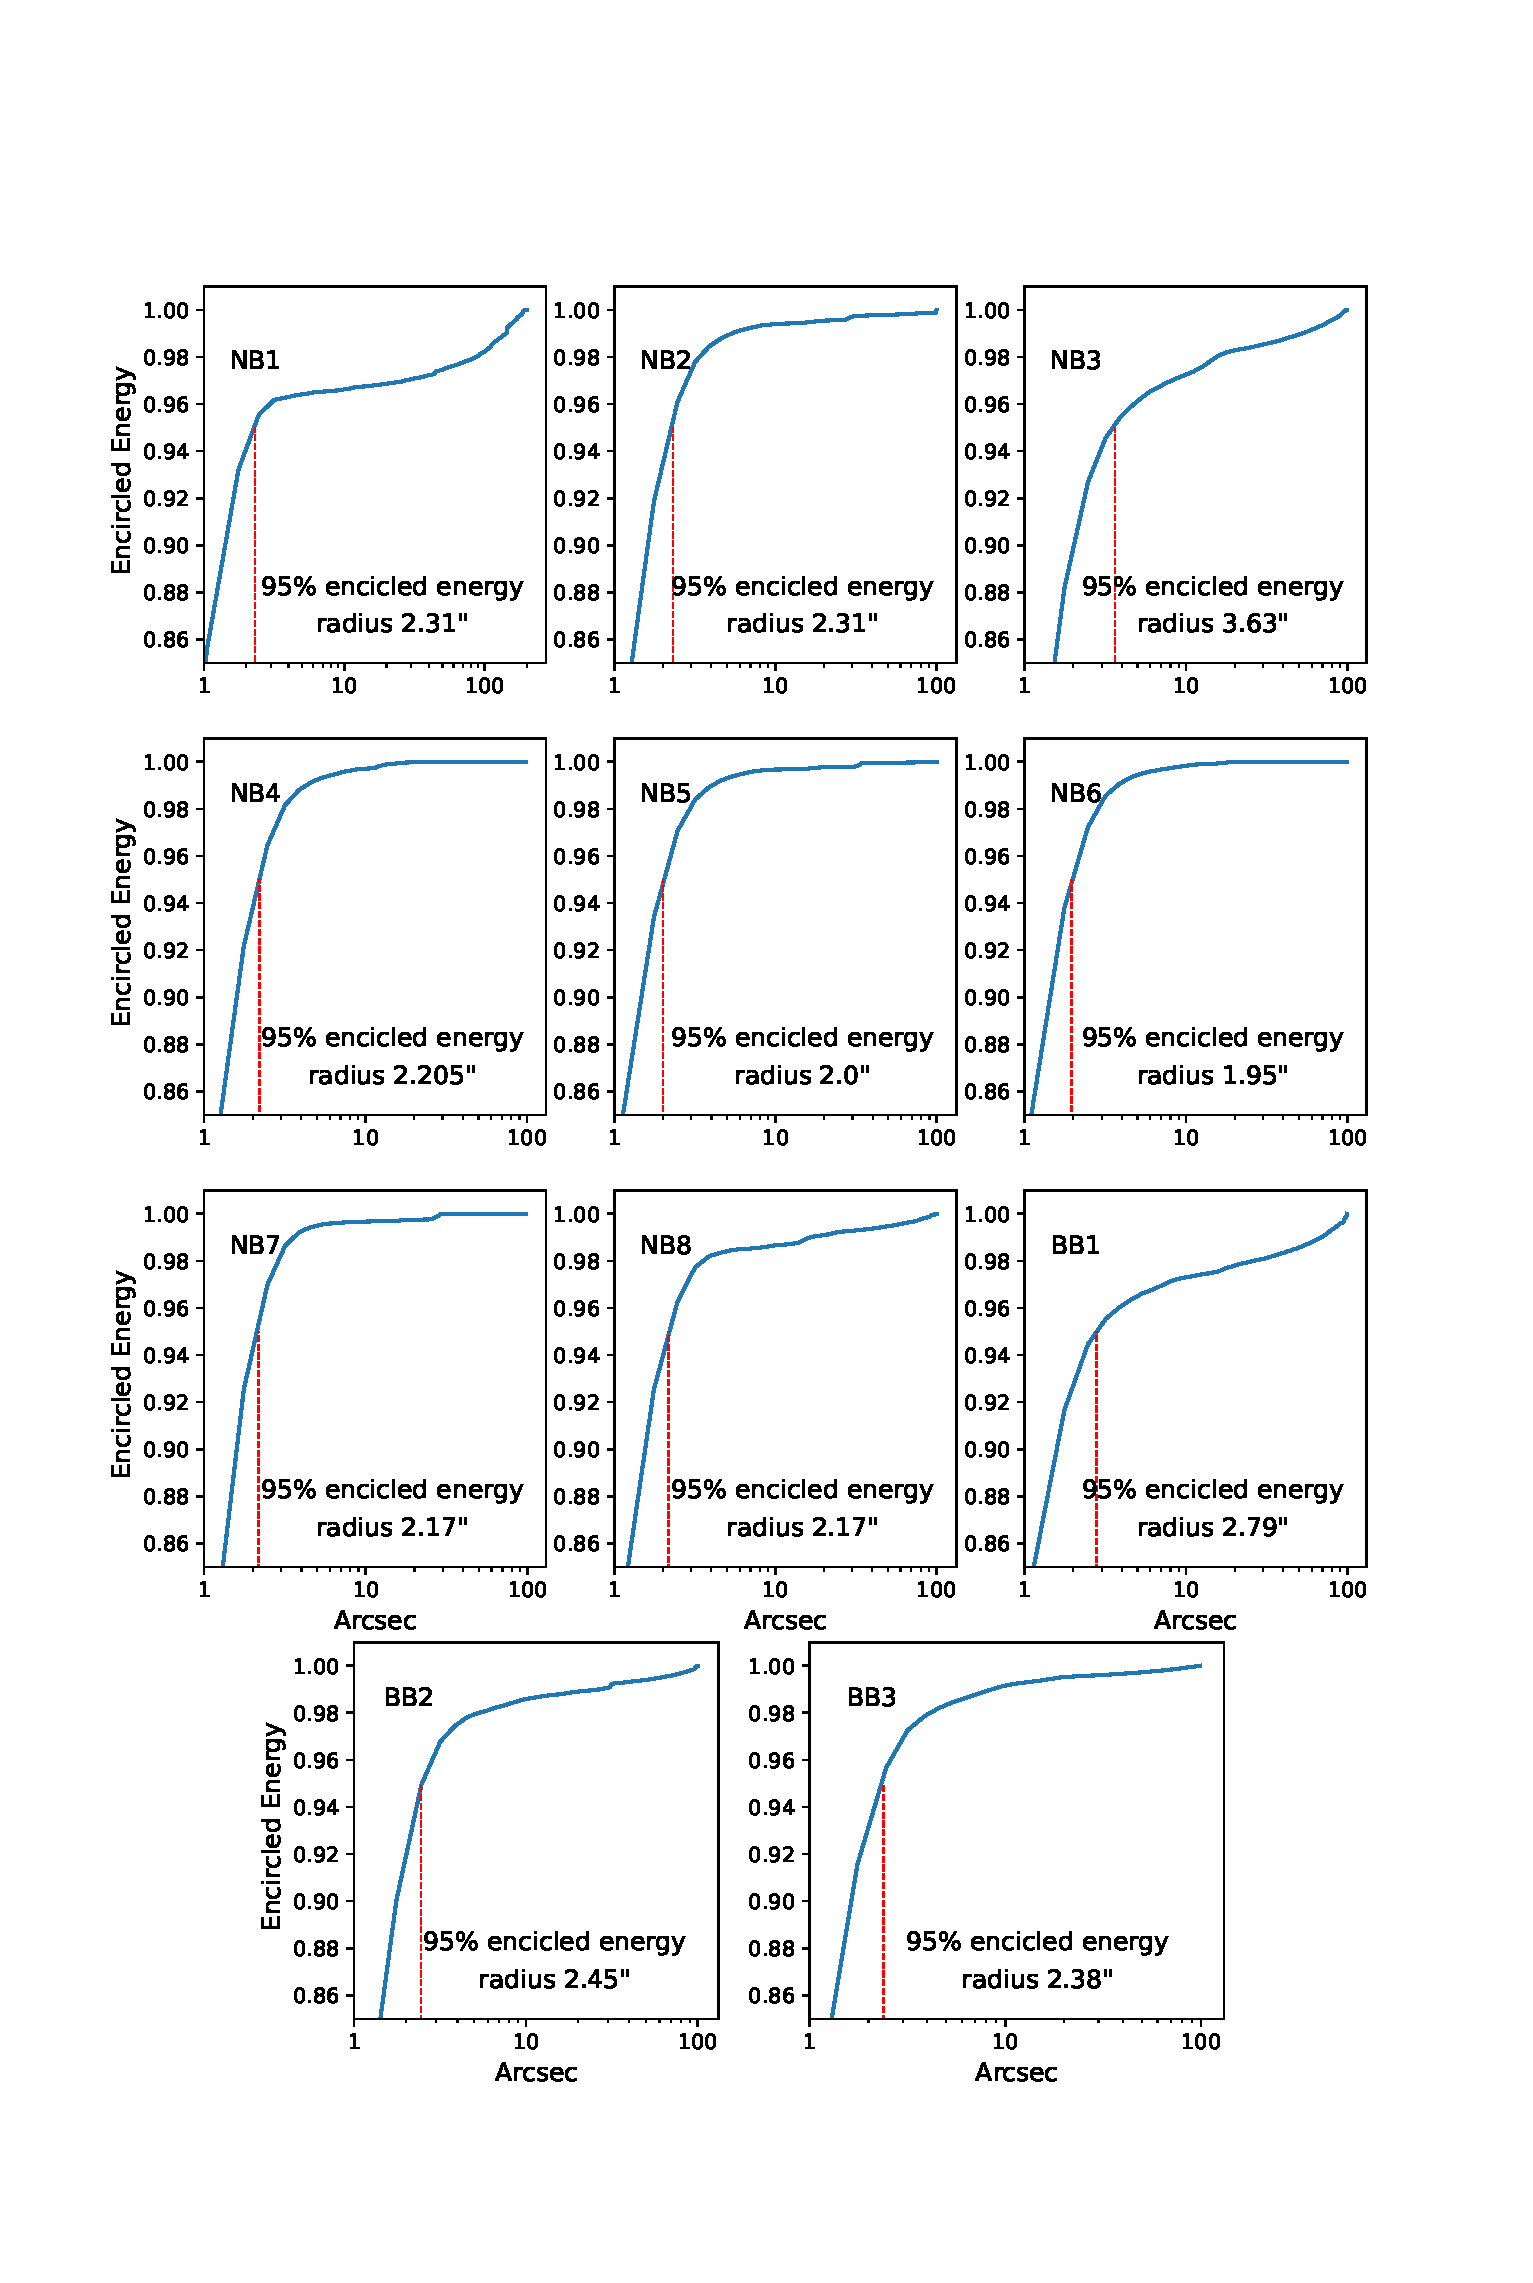
\includegraphics[trim={1.5cm 3cm 2.5cm 4cm},clip,width=0.85\textwidth]{psf_ese_2.eps}
    \caption{The encircled energy curve for the measured PSF. The 95\% encircled energy radius are marked with the vertical dashed red line. The angular scale of the 95\% encircled energy radius is also quoted in each panel for the specific filter combination.}
    \label{fig:psf_ese}
\end{figure*}
%%---------------------------%%

%%---------------------------------------------------
\subsection{Effective Area of SUIT}\label{eff_area}
%%---------------------------------------------------
Let $p(\lambda)$ be the incident photon flux on the entrance aperture. The photo-electron count at the detector, also known as Data Number (DN) is given by,

 $$   DN=\int~p(\lambda)~R(\lambda)~t~d\lambda $$

\noindent where $R(\lambda)$ is the instrument effective area for the specific filter combination and $t$ is the exposure time. The instrumental response, $R(\lambda)$, is computed by multiplying the measured response of all the optical components along the ray path. 

Hence,
    $$ R(\lambda)~=~TF(\lambda)\times PM(\lambda)\times SM(\lambda)\times SF_{i}(\lambda)\times $$
    $$ CF(\lambda)\times L(\lambda)\times QE(\lambda) \times A$$

\noindent where A is the entrance aperture area and TF($\lambda$), PM($\lambda$), SM($\lambda$), SF$_{i}$($\lambda$), CF($\lambda$), L($\lambda$) and QE($\lambda$) are the measured responses as a function of wavelength of thermal filter, primary mirror, secondary mirror, science filters, band pass filters, field corrector lens and the quantum efficiency of the CCD, respectively. The obtained effective area curves for each filter are shown in Fig.~\ref{fig:eff_area}. 

%%---------------------------------------------------------------
\begin{figure*}
    \begin{center}
        \begin{tikzpicture}[node distance=2cm]
            \node(muram)[io]{Model 3D atmospheres simulated by the radiative-MHD code MURaM};
            \node(slice)[io,right of=muram,xshift=3.5cm]{Slice the MURaM cubes and interpolate them to various $\mu$ values};
            \node(filter)[io,below of=muram,yshift=-1cm]{Use \suit~ science filter profiles accounting for all the optics on the ray path};
            \node(odf)[io,right of=filter,xshift=3.5cm]{Generate ODF tables for various filters using the MPS-ATLAS code};
            \node(rdt)[io,right of=odf,xshift=3.5cm,yshift=1.5cm]{Use ODF tables and 1D ray-atmospheres from the 3D MHD cube to carry out RT calculations using MPS-ATLAS};
            \node(int)[io,below of=rdt,yshift=-3.5cm]{Integrate the generated spectra for each pixel of the cube over the wavelength range of the filter profile to generate the intensity map};
            \node(conv)[io,left of=int,xshift=-4.5cm]{Convolve the total emergent intensity maps with relevant \suit~ PSF and bin to \suit~ plate scale to create mock observation};
            \draw[arrow](muram)--(slice);
            \draw[arrow](slice)--(rdt);
            \draw[arrow](filter)--(odf);
            \draw[arrow](odf)--(rdt);
            \draw[arrow](rdt)--(int);
            \draw[arrow](int)--(conv);
        \end{tikzpicture}
        \caption{The flow chart shows the entire process of generating the simulated intensity maps, from the data cubes and characterizing the filters.}
        \label{fig:flow}
    \end{center}
\end{figure*}
%%---------------------------------------------------------------

%%---------------------------------------------------------------
\subsection{The Point Spread Function (PSF) of {\suit}} \label{sec:psf}
%%-----------------------------------------------------------------
In Fig.~\ref{fig:psf_3d}, we plot the measured Point Spread Function (PSF) at the centre of the CCD for the different science filter combinations for {\suit}. The PSFs are highly peaked at the centre. The scattered light background becomes clearly visible due to the log scaling of the color bar and is more than two orders of magnitude lower than the peak.

Fig.~\ref{fig:psf_ese} shows the encircled energy curve for the measured PSFs for various filter combinations normalized to the total integral of unity. The vertical dashed lines in each plot show the radius within which 95\% of the incident light falls. For example, for the NB02 filter, 95\% of the incident light from a point source arrives within a 2.31{\arcsec} radius ($\sim$ 4.6{\arcsec} diameter) and 5\% of the light falls outside that region. Note that while the 95\% diameter is 4.6{\arcsec}, the PSF is strongly peaked. The overall diameter is considerably larger than the highly peaked part of the PSF because of the presence of a pedestal in the PSF. The pedestal is visible in all of the cases at the base of the central peak, although it is about 2 order of magnitude lower in all the cases (see Fig.~\ref{fig:psf_3d}). In some cases (e.g. NB01, BB02 etc.) a few or multiple smaller peaks apart form the pedestal are also visible. Similar radii for other filters are quoted in the corresponding panels of Fig.~\ref{fig:psf_ese}. The encircled count curves help us characterize the stray light for various filter combinations.

%%%%%%%%%%%%%%%%%%%%%%%%%%%%%%%%%%%%%%%%%%%%%%%%%%%%%%%%%%%%%%%%
\section{Forward Modeling SUIT intensity maps using MPS-ATLAS and MURaM} \label{sec:mps}
%%%%%%%%%%%%%%%%%%%%%%%%%%%%%%%%%%%%%%%%%%%%%%%%%%%%%%%%%%%%%%%%

One of the essential steps of characterizing the science filters was to conduct a thorough throughput modeling for the concerned filter combinations. However, quantifying the effects of the wavelength response of the optical components and the PSF on the spatially resolved observations, as well as the contrast variation, requires detailed modeling with resolved simulations of the Sun's surface. For this purpose, we use the MPS-ATLAS code. It is an updated version of the well established ATLAS9 \citep{atlas9} code that can efficiently generate Opacity Distribution Functions (ODFs), model atmospheres, and calculate emergent spectra in local thermodynamic equilibrium (LTE) for a given wavelength range by solving radiative transfer (RT) equation in plane parallel geometry using the assumptions of local-thermodynamic-equilibrium (LTE).

%%----------------------------------------------------------
\begin{figure}
    \centering
    \includegraphics[width=.85\textwidth]{mps.pdf}
    \caption{Forward modelled intensity maps at various $\mu$ values for BB02 filter of SUIT.}
    \label{fig:flux_maps}
\end{figure}
%%----------------------------------------------------------

%%----------------------------------------------------------
\begin{figure}
    \centering
    \includegraphics[trim={0cm 6cm 0cm 5cm}, clip, width=.85\textwidth]{mps_sim.pdf}
    \caption{Forward modelled intensity maps for various science filters of SUIT.}
    \label{fig:flux_maps_filt}
\end{figure}
%%----------------------------------------------------------

We use 3D MHD model atmospheres simulated by \cite{rempel20} and 1.5D RT with MPS-ATLAS \citep[see e.g.,][for details]{anusha21} with measured filter profiles of {\suit}, to calculate the emergent intensity. The 3D MHD simulation employs a symmetric lower boundary condition for the magnetic field and a variety of initial magnetic field configurations to create small-scale variations and various levels of magnetization. The RT equation is solved using the method of ODFs, accounting for both continuum and line opacities within the concerned wavelength range. This takes into account both continuum and line opacity within the concerned wavelength range. Accurately accounting for the line opacity is one of the major challenges in synthesizing spectra over a broad wavelength range. In the ODFs method, the opacity is sorted without the information of the corresponding wavelength within small intervals of wavelengths known as bins. The geometric mean of the sorted opacity values for multiple sub intervals within a given wavelength bin is pre-tabulated over atmospheric parameters such as temperature, pressure and micro-turbulent velocities. During RT calculations, opacity is then interpolated for the required grid parameters of the atmospheric model. The primary goal of the ODF method is to significantly minimize the computational time required for RT calculations. This becomes particularly crucial when computing emergent spectra across numerous atmospheres, such as those arising from 3D MHD simulations. 

\cite{anusha21} developed an optimized method using the MPS-ATLAS code that allows us to use an arbitrary filter profile instead of a rectangular filter profile. We use this method, with our measured effective area, to forward model intensity maps for NB01, NB02, NB05, NB06, NB07, BB01, BB02 and BB03 filter combinations that {\suit} is using.

We describe the end-to-end procedure in Figure~\ref{fig:flow}. The 3D MHD model atmospheres are sliced at various angles and interpolated to various Line of sight (LOS) angles. As described earlier, the ODF tables are generated for various atmospheric parameters, such as temperature, pressure and micro-turbulent velocities, for the measured science filter profiles. The generated ODF tables are used to solve the RT through the model atmosphere using the MPS-ATLAS code. This provides us the emergent intensity as a function of wavelength for all the rays of the model atmosphere. Integrating this intensity across the wavelength range, we determine the total emergent intensity for each filter.

Figure~\ref{fig:flux_maps} displays the {\suit}'s BB02 intensity maps obtained at various $\mu$ values, namely $\mu$~=~1.0, 0.8, 0.7 and 0.6, respectively. The spatial scale of the region is $(9~\textrm{Mm}\times9~\textrm{Mm})$ with $(512\times512)$ pixels, with a pixel size of $\simeq 0.025{\arcsec}/\textrm{pixel}$. This is at a much higher resolution than that of {\suit}, which is $\sim \textrm{0.7"/pixel}$. Moreover, these intensity maps do not include the effects of the instrument point spread function (PSF). Therefore,  we first need to convolve the computed intensity maps with the measured PSF of {\suit}, and then bin it to {\suit} plate scale to obtain synthetic observables that are comparable to {\suit} observations. Fig.~\ref{fig:flux_maps_filt} displays the simulated intensity maps for the {\suit} BB filters across the same MURaM cube.

We use the MURaM and MPS-ATLAS codes to forward model the observations for NB01, NB02, NB06, NB07, BB01, BB02 and BB03. We note that since the MURaM simulations studied here cannot be used for the chromospheric filters, namely NB03 (\ion{Mg}{2}~k), NB04 (\ion{Mg}{2}~h) and NB08 (\ion{Ca}{2}~k), we have used observations recorded by~{\it IRIS} to forward model the NB03 and NB04 filter observations.~{\it IRIS} also provides spectra corresponding to the continuum filter NB05. Hence, we forward model NB05, also using~{\it IRIS} observations. Forward modelling of SUIT observations using~{\it IRIS} data is straightforward as we do not need to use any MHD simulation cube and RT code. However, the convolution with the spatial PSF and the application of the spectral filter profile, etc. still must be carried out. For our analysis, we use dense raster scans from~{\it IRIS}. The dense rasters usually have $\sim$ 0.33{--}0.4 \arcsec per pixel spatial resolution. This spatial resolution is half of the pixel size of \suit. In addition to that, the 95\% encircled energy radius for most of the \suit~filter combinations is $\sim$ 2\arcsec. Hence, we can safely ignore the instrument characteristics of~{\it IRIS}. For the two filters where we are using~{\it IRIS} data, the bottom right box in Fig.~\ref{fig:flow} is replaced by~{\it IRIS} observations.

%%----------------------------------------------------------------------------
\begin{figure}
    \centering
    \includegraphics[trim={5cm 1cm 5cm 2.7cm},clip,width=0.85\textwidth]{BB3_convolve.pdf}
    \caption[The effects of convolution on the simulated BB03 intensity map]{The effects of convolution on the simulated BB03 intensity map. Panel a) MPS-ATLAS simulated BB03 intensity map. Panel b) convolved and binned BB03 intensity map. The normalized intensity variation along the horizontal and vertical black lines are plotted in panel c and d, respectively. The blue curves correspond to the simulated BB03 filter, whereas the orange curves correspond to convolved binned data.}
    \label{fig:BB3_conv}
\end{figure}
%%----------------------------------------------------------------------------

%%-------------------------------------------------------------------------
\subsection{{\suit} filters forward modeled with MPS-ATLAS}\label{sec:mps_contrast}
%%-------------------------------------------------------------------------

Following the procedure described above, we forward model the intensity maps in  NB01, NB02, NB06, NB07, BB01, BB02 and BB03. Since the spatial extent of the simulation box is much smaller compared to the size required to reliably convolve with the {\suit} PSF, we stitched the same simulated box multiple times to be able to convolve with the measured PSFs of SUIT. This could be done without problems due to the use of periodic boundary conditions in the MURaM simulation setup. Fig.~\ref{fig:BB3_conv}.a displays the stitched images obtained for BB03. In Fig.~\ref{fig:BB3_conv}.b, we display the corresponding image that is convolved with the PSF of the respective filter of SUIT and binned to its plate scale.

To compare the intensity contrast before and after the convolution, we plot intensity across a small part of the vertical (panel c) and a horizontal cut (panel d). The blue curves represent the intensity cut through the MPS-ATLAS simulated intensity maps, while the orange dashed curves are for convolved-binned intensity maps. The contrast variation across the cuts reproduces the intensity peaks and troughs in similar regions. These intensity cuts demonstrate that we can reproduce the intensity contrasts in the forward-modelled data with reasonably similar spatial positions. The forward-modelled observational features appear broader, with reduced contrast. This reduction in contrast, is anticipated given the difference in the plate scale of simulation and that of forward-modelled observations. The 95\% encircled energy is largely ~ 2{\arcsec} for most filter combinations (see Fig.~\ref{fig:psf_ese}). This would imply that the intensity from a point source would be redistributed to a circle of 2{\arcsec} radius. So, if we have two equally bright/dark point sources, they would be merged if the distance between them is 2{\arcsec} or less. Hence, we should be able to study contrast variation at the spatial scale of $\sim$ 2{\arcsec} using {\suit} observations. We have performed this exercise on all the filters corresponding to the photosphere and continuum and have obtained similar results.

%%----------------------------------------------------------------------------
\subsection{NB03 \& NB04}\label{sec:nb3_contrast}
%%----------------------------------------------------------------------------

As alluded earlier, to forward model NB03 and NB04 observations, we have used~{\it IRIS} archival data. The~{\it IRIS} obtains UV spectra with high spatial (0.33{--}0.4{\arcsec} per pixel), temporal (1s), and spectral resolution ($\sim$26 and $\sim$53~m{\AA}) and images of the scanned regions using the slit-jaw imager. In the spectral channels, the strongest lines that~{\it IRIS} regularly observes are \ion{C}{2}, \ion{Mg}{2} and \ion{Si}{4}. Here we use the very large and dense 320 step raster observation from 11th July, 2023 of a sunspot in AR 13363. The sunspot was located at the heliographic position of $\sim [-180\arcsec,-397\arcsec]$. The~{\it IRIS} raster had a FoV of $\sim [112\arcsec,175\arcsec]$. We use \textit{iris\_getwindata.pro} available in the \textit{sswidl} distribution to get the calibrated spectra over the raster FoV. This gives us the calibrated spectra for all the pixels in the raster FoV in units of $erg.cm^{-2}.s^{-1}.sr^{-1}.pix^{-1}$. We multiply the entire spectra of each pixel through the NB03 and NB04 effective area (see            
Fig.~\ref{fig:eff_area} panel b) and convolve with the measured PSF (see            Fig.~\ref{fig:psf_3d}) to forward model NB03, NB04 observations. Consequently, the observed intensity is, 

$$DN_{NB03}~=~\int~{\it IRIS}\_spec(\lambda)~R_{NB03}(\lambda)~t~d\lambda$$
and 
$$DN_{NB04}~=~\int~{\it IRIS}\_spec(\lambda)~R_{NB04}(\lambda)~t~d\lambda$$

\noindent where $R_{NB03}$ and $R_{NB04}$ are the measured effective area for the respective filter combinations. Fig.~\ref{fig:nb3_conv}.a shows the~{\it IRIS} raster FoV intensity map in the \ion{Mg}{2}~k line. The~{\it IRIS} image convolved with NB03 (NB04) PSF and binned to the {\suit} plate scale is shown in Figs.~\ref{fig:nb3_conv}.b(c).

To compare the intensity contrast obtained from SUIT images with those from~{\it IRIS} observations, in Figs.~\ref{fig:nb3_conv}.e \& f, we plot the normalized intensity profiles along the vertical (panel d) and horizontal (panel e) lines shown in panels a, b and c for NB03 and NB04 as labelled. The horizontal white dotted line encounters a light bridge on the western end of the sunspot (marked with a white arrow in Fig.~\ref{fig:nb3_conv} panels a, b \& c). We see three dips in the intensity profile in Fig.~\ref{fig:nb3_conv} panel e, as the horizontal white dotted line encounters the sunspot thrice. In both panels d \& e, NB03 (orange dashed line) and NB04 (black dot dashed line) has a lower contrast (peak to trough variation) compared to~{\it IRIS} (red solid line) and NB04 (black dot-dashed line) contrast. This is in line with our measurements of the PSF for NB03 \& NB04, as the measured PSF for NB03 has a higher scatter component in the background compared to NB04 (see panel c \& d in Fig.~\ref{fig:psf_3d}, Fig.~\ref{fig:psf_3d}). Therefore,  NB03 has a higher radius for 95\% encircled count (see NB03 and NB04 in Fig.~\ref{fig:psf_ese}). A higher radius for 95\% encircled count results in lower contrast in the convolved mock NB03 map.

%%%%%%%%-----------------%%%%%%%%%%%%%%%
\begin{figure}
    \centering
    \includegraphics[trim={5cm 0.6cm 6cm 0cm},clip,width=0.85\textwidth]{nb3_conv_edit.pdf}
    \caption[Effects of convolution on the~{\it IRIS} raster observation with the NB03 \& NB04 PSF]{Effects of convolution on the~{\it IRIS} raster observation with the NB03 \& NB04 PSF. Original (panel a), convolved with NB03 PSF and binned to {\suit} plate scale (panel b), convolved with NB04 and binned (panel c)~{\it IRIS} intensity maps obtained in \ion{Mg}{2}~k. Normalized intensity variation along the vertical-solid (horizontal-dashed) white line marked in panel a, b \& c are shown in panel d (panel e). Red-solid curves correspond to original~{\it IRIS} image, orange-dashed curves correspond to mock NB03 and black dot-dashed curves correspond to NB04.}
\label{fig:nb3_conv}
\end{figure}
%%%%%%%%-----------------%%%%%%%%%%%%%%%

%%-------------------------------------------
\subsection{NB05}\label{sec:nb5_contrast}
%%-------------------------------------------

The NB05 channel (with the central wavelength at 283.2~nm) is also observed by~{\it IRIS}. Therefore, we use the~{\it IRIS} 2832~{\AA} window observation of the same AR~13363 mentioned in \S\ref{sec:nb3_contrast}. %We use \textit{iris\_getwindata.pro} to get the spectra of the pixels in the raster FOV in units of $erg.cm^{-2}.s^{-1}.sr^{-1}.pix^{-1}$. Similarly, the whole spectrum is passed through the measured NB5 effective area and convolved with the measured PSF. 
In Fig.~\ref{fig:nb5_conv}.a, we plot the integrated intensity of the~{\it IRIS} 2832~{\AA} window. In panel b we plot the same region passed through the NB05 effective area and convolved and binned to {\suit} plate scale. In panels c and d we plot the normalized~{\it IRIS} intensity (red solid line) and normalized {\suit} NB05 intensity (orange dashed line) along the white dashed line and blue solid line marked in panels a and b, respectively. The features marked (`1' \& `2') in panels a and b are also marked in the normalized intensity variation panel e. Although there is a significant loss in contrast, the features are still identifiable. As demonstrated previously, various features are reproduced in the same spatial location with reduced contrast.

%%%%%%%%-----------------%%%%%%%%%%%%%%%
\begin{figure}
    \centering
    \includegraphics[trim={0.5cm 0.2cm 2cm 0cm},clip,width=0.85\textwidth]{NB5_feature_1.pdf}
    \includegraphics[trim={2.7cm 0.2cm 3cm 2cm},clip,width=0.95\textwidth]{NB5_feature_2.pdf}
    \caption[Effects of convolution on the~{\it IRIS} raster observation with the NB05 PSF]{Effects of convolution on the~{\it IRIS} raster observation with the NB05 PSF. We plot the~{\it IRIS} raster intensity map obtained in 2832~{\AA} continuum in panel a and the convolved-binned intensity image in panel b. 
    The normalized intensity variation obtained from both images along the white-dashed and blue-solid lines are shown in panels c and d, where red solid lines correspond to the original~{\it IRIS} image and orange dashed lines correspond to the convolved-binned intensity map. The two thin features marked by `1' and `2' within the sunspot in panels a and b are also marked in the intensity variation plot.}
\label{fig:nb5_conv}
\end{figure}
%%%%%%%%-----------------%%%%%%%%%%%%%%%

We have also used a very large, dense 320-step raster observation from 20th July 2023 of a sunspot in AR 13376 to create the mock observation. The sunspot was located at the heliographic position of $\sim [-147",325"]$. The~{\it IRIS} raster had a field of view (FoV) $\sim [112",119"]$. As described earlier, we forward modeled SUIT observations in the NB05 passband for this region. In Fig.~\ref{fig:nb5_conv_1} panel a we plot the integrated map obtained in~{\it IRIS} 2832~{\AA} window. In panel b we plot the same region passed through the NB05 effective area and convolved-binned to the {\suit} plate scale. In panel c(d) we plot a cropped view of the sunspot in the southern part of the region in~{\it IRIS} 2832~{\AA} ({\suit}~NB05 convolved). The light bridge within this sunspot narrows in thickness as we move from the upper-left to the lower-right. We take multiple measurements close to one another and average them to calculate the thickness of the light bridge at some specific location. In the northern part, the lightbrdge is $\sim 2\arcsec$ thick in the~{\it IRIS} observation and 4$\arcsec$ in the mock NB05 observation (see upper set of white arrows in panels c and d). It narrows down to 1$\arcsec$ in the southern part in the~{\it IRIS} observation, and 1.8$\arcsec$ in the mock NB05 observation (lower set of white arrows).

We take a slice through the sunspot and the light bridge, marked with a vertical white line in Fig.~\ref{fig:nb5_conv_1} panel c. The intensity along this line for normalized~{\it IRIS} contrast (solid red line) and convolved NB05 contrast (dot-dashed blue line), is plotted in Fig.~\ref{fig:nb5_conv_1} panel e. The light bridge is marked with a black arrow in the intensity profile.

%%%%%%%%-----------------%%%%%%%%%%%%%%%
\begingroup
    \centering
    \includegraphics[trim={3cm 4cm 3cm 0cm},clip,width=0.85\textwidth]{suit_sunspot_part1.pdf} \\
    \includegraphics[trim={1cm 0.2cm 1cm 1cm},clip,width=0.85\textwidth]{suit_sunspot_contrast_2.pdf}
    \captionof{figure}[Effects of convolution on the~{\it IRIS} raster observation with the NB05 PSF]{Effects of convolution on the~{\it IRIS} raster observation with the NB05 PSF. Panel (a):~{\it IRIS} raster intensity in 2832~\AA\ continuum.A large sunspot with a thin, light bridge in the middle is present in the southern part of the region. Panel (b): The~{\it IRIS} raster observation in panel a convolved with the NB05 PSF (see fig.~\ref{fig:psf_3d} panel e). Panel (c) \& (d): Zoomed view of the larger sunspot in the South in~{\it IRIS} and the simulated \suit\ NB05 map, respectively. The light bridge in the middle of the sunspot is marked by a set of four white arrows. The thickness of the light bridge at two locations is marked in both the panels. The normalized intensity along the vertical  white line drawn in panel (c) is plotted in panel (e). The normalized intensity of the original~{\it IRIS} (mock NB05) observation is plotted in solid red (dot-dashed blue) line. The light bridge is marked in the intensity profile with a black arrow.}
    \label{fig:nb5_conv_1}
\endgroup
%%%%%%%%-----------------%%%%%%%%%%%%%%%

%%%%%%%%%%%%%%%%%%%%%%%%%%%%%%
\section{Summary and Conclusions}\label{sec:con}
%%%%%%%%%%%%%%%%%%%%%%%%%%%%%%

The observation of any optical telescope is convolved by the PSF of the telescope. The PSF represents the response of the optical system to a point source. It quantifies the extent of blurring of a point source when imaged through the optical system, as well as the effects of various components like scattering, diffraction, etc. We have applied the measured PSF at the \suit\ detector plane for various filter combinations to the emergent radiation from MURaM simulation cubes (computed by MPS-ATLAS) and to pre-existing~{\it IRIS} observations to create mock {\suit} observations. The {\suit} PSF in all of the filter combinations is highly peaked with a pedestal $\sim$ two orders of magnitude lower (see Fig.~\ref{fig:psf_3d}). In most of the filter combinations the 95\% encircled count radius is $\sim$ 1.4 {--} 2.5{\arcsec}. This would imply that two equally bright or dark features on the Sun $\sim$ 2{\arcsec} apart would be merged in the corresponding {\suit} observation. Hence, we could resolve features on a spatial scale of $>$ 2.5{\arcsec} for the corresponding filters in {\suit} observations. These projections are more relevant for line filters in {\suit} (e.g. NB03(\ion{Mg}{2} k), NB04(\ion{Mg}{2} h, NB08 (\ion{Ca}{2} h)), as it would exhibit more features in close proximity (bright points in ARs and QS, the plage regions around sunspots, small eruptions in ARs). These projections are made with the measured PSF at the center of the CCD. The PSF distortions increase gradually as we move away from the centre of the CCD, with more angular elongation. 

We believe the forward modeling pipeline will help us simulate {\suit} observations from existing MHD simulations and compare them to real {\suit} observations to constrain current model parameters. The comparisons with forward-modelled mock {\suit} observation with real {\suit} observations over time would also provide useful insights into the degradation of the instrument with respect to the on-ground projections. The deconvolution algorithm would be useful to improve the contrast across {\suit} observations and spatially localize features more reliably on the solar surface.
%
\chapter{Intital preparatory analysis for SUIT}\label{c:chap5}

\chaptermark{SUIT preparatory analysis}
\begin{quote}
    { \em~~~~~~~This thesis chapter originally appeared in the literature as} \\
{{\em {\bf Photometric calibration and spectral validation of
the Solar Ultraviolet Imaging Telescope onboard
Aditya-L1}, Sarkar, J., Roy, S., Ramaprakash, A.N., et. al.,  2025,  J. Astron. Telesc. Instrum. Syst. 11(1), 014005 (2025), doi:\href{https://www.spiedigitallibrary.org/journals/Journal-of-Astronomical-Telescopes-Instruments-and-Systems/volume-11/issue-1/014005/Photometric-calibration-and-spectral-validation-of-the-Solar-Ultraviolet-Imaging/10.1117/1.JATIS.11.1.014005.short}{10.1117/1.JATIS.11.1.014005}.}
\end{quote}
\justifying

%%%%%%%%%%%%%%%%%%%%%%%%%%%%%%%%%%%%%%%%%%%%
\section{Introduction}\label{secc3_intro}
%%%%%%%%%%%%%%%%%%%%%%%%%%%%%%%%%%%%%%%%%%%%

\suit~consists of two main sub-units: The \suit~optics package - comprising an off-axis Ritchey-Chr\'{e}tien telescope, and \suit~Electronics package - responsible for imaging with the telescope and communicating with the satellite. The main components of the \textit{SUIT} optics package include a multi-operation entrance door, a thermal filter to limit the amount of incoming sunlight, primary and secondary mirrors, a shutter mechanism to control exposure times, baffles to reduce stray and scattered light, a motorized filter wheel assembly, a piezoelectric focusing mechanism, and a CCD detector. Figure \ref{fig:suit} shows a schematic diagram of the telescope (For further details, please refer to \cite{suit_main}).

%%%%%%%%%%%%%%%%%%
\begin{figure}[ht!]
    \centering
    \includegraphics[width=0.8\textwidth]{SUITLayout.jpg}
    \caption{Schematic diagram of the \textit{SUIT} telescope.}
    \label{fig:suit}
\end{figure}
%%%%%%%%%%%%%%%%%%

\suit~observes the Sun in eleven spectral bands, of which three are broadband (referred to as BB) and eight are narrow bands (referred to as NB), as listed in Table~\ref{tab:science_filters}. These are used to image different heights of the solar atmosphere, from the photosphere to the chromosphere. In the wavelength range of interest, i.e., 200{--}400 nm, the solar flux increases by two orders of magnitude, as can be seen in the combined spectrum obtained from solar flux measured by SOLSPEC (see Fig.~\ref{fig:sun_spec}). {\bf Therefore, we must employ certain combination filters to control solar flux levels and achieve the best signal-to-noise ratio (SNR) at each bandpass within the nominal exposure time while maintaining the spectral purity of the passband by suppressing leakage of light from wavelength bands outside of the science interest.} These combination filters are listed in the second column of Table~\ref{tab:science_filters}. In total, \textit{SUIT} has 16 filters mounted on two filter wheels, each having eight slots. A given filter combination is achieved by rotating the two filter wheels independently and placing the desired filter combination in the beam path. {\bf For example, \textit{SUIT} uses BB1 as a combination filter for BB1, as this particular filter aims to measure the irradiance of the entire Herzberg Continuum. On the other hand, the NB8 filter aims to accurately observe the line core of the \ion{Ca}{2}~h line ($\sim$396.85~nm). Several strong flare lines close to the line core go into emission during a flare (e.g. $\mathrm{H\epsilon}$ at $\sim$ 397~nm). Combining NB08 with another NB8 results in lower SNR for a given exposure time, as opposed to combining it with a bandpass filter. But we decided to chose this combination for maintaining the spectral purity at the expense of cadence or SNR. Similar choices regarding spectral purity were made for the band NB7 (CN Band), where we specifically wanted to probe the CN band in the continuum. The position of the various filters on the filter wheel also plays an important role in dictating the cadence of the observations, e.g. the BB filters are usually not planned to be used in normal flare observations. So, the NB filters and their corresponding combination filters have to be arranged in such a way as to minimize the time taken to rotate the filter wheel, achieve the planned filter combination, and maintain an acceptable cadence. The choice of filter combination is a delicate optimization between suppressing the out-of-band leakage and achieving a reasonable SNR within an acceptable exposure time. Additionally, the positions of combination filters on the filter wheel must be chosen to minimize the time spent in rotating the filter wheels from one combination to other dictating the cadence of observation.}

%------------------------------------------------------------
\begin{figure}[ht!]
    \begin{center}
    \begin{tabular}{c}
    \includegraphics[trim={0.8cm 0.3cm 2cm 2.2cm},clip,width=0.8\linewidth]{solar_spec_3.pdf}
    \end{tabular}
    \end{center}
\caption[The solar spectrum obtained from SOLSPEC.]{The solar spectrum from SOLSPEC. Parts of the solar spectra marked in red show the wavelength range covered by {\suit}'s observation passbands. The inset plot shows a dramatic rise in solar irradiance within \suit's observation band. } 
\label{fig:sun_spec} 
\end{figure} 
%-----------------------------------------------------------


%-----------------------------------------------------------
\begin{table}[ht!]
\begin{center}
\resizebox{0.8\textwidth}{!}{%
\begin{tabular}{||l|c|c|c|r||}
\hline
\textbf{Science}  &	\textbf{Combination} &	\textbf{Central} & \textbf{Bandpass} &\textbf{Science} \\
\textbf{Filter}	&	\textbf{Filter}     &	\textbf{Wavelength  (nm)}	&		\textbf{(nm)	}	   	&\textbf{target}		\\
\hline
NB1     & BB1 		& 214.0 		    & 11.0 		& Continuum\\
NB2 	& BP2		& 276.7				& 0.4 		& Mg~\rm{II}~k blue wing \\
NB3 	& BP2		& 279.6 			& 0.4 		& Mg~\rm{II}~k\\
NB4 	& BP2		& 280.3				& 0.4 		& Mg~\rm{II}~h\\
NB5		& BP2		& 283.2				& 0.4 		& Mg~\rm{II}~h red wing\\
NB6 	& BP3		& 300.0 			&1.0 		& Continuum\\
NB7 	& BP3		& 388.0				&1.0 		& CN Band\\
NB8		& NB8		& 396.85 			& 0.1 		& Ca~\rm{II}~h\\
BB1 	& BB1		& 220.0				& 40.0		& Herzberg Continuum \\
BB2 	& BP4		& 277.0 			& 58.0       & Hartley Band\\
BB3 	& BP4		& 340.0				& 40.0        & Huggins Band\\
\hline
\end{tabular}}
\end{center}
\caption[Science filters on-board {\suit}]{List of science filters on board \suit. Columns from left to right denote filter mnemonics (including science and combination filters; NB: Narrowband, BB: Broadband, BP: Bandpass), central wavelengths for science filters and corresponding bandpasses, and the observation interest for the filter.} 
\label{tab:science_filters}
\end{table}
%-----------------------------------------------------------

%%%%%%%%%%%%%%%%%%%%%%%%%%%%%%%%%%%%%%%%%%%%
\section{Analysis of Spacecraft jitter simulation for {\suit}}\label{sec:suit_jitter}
%%%%%%%%%%%%%%%%%%%%%%%%%%%%%%%%%%%%%%%%%%%%

One of the key steps in estimating the imaging performance was to quantify if the RMS level of spacecraft jitter would affect the imaging across various exposure times. For this purpose, we analyzed the simulated spacecraft drift data provided by the ISRO URSC team to quantify the RMS jitter as a function of exposure time. Two main moving components within the payload can generate significant jitter on the payload, namely the shutter vane and the filter wheel (FW) movement. The spacecraft has a filter wheel movement torque compensator in place to minimize the jitter generated by the FW movement. So, four main scenarios were simulated to be analyzed, arranged from least to most amount of jitter:

%%%
\begin{enumerate}
    \item No shutter torque + no filter movement
    \item Only shutter torque
    \item Shutter torque + FW movement + FW compensation torque
    \item Shutter torque + FW movement + no FW compensation torque
\end{enumerate}
%%%

%%%%%%%%
\begin{figure}[ht!]
    \centering
    \includegraphics[trim={1cm 0cm 1cm 1cm},clip,width=0.9\textwidth]{jitter_sim.pdf}
    \caption[Simulated drift for the yaw, roll and pitch axis as a function of time.]{The simulated drift for the yaw (blue solid), roll (red dashed) and pitch (green dot-dashed) axis of the payload as a function of time for the aforementioned four cases in \S\ref{sec:suit_jitter} in the four panels respectively as marked.}
    \label{fig:jitter_sim}
\end{figure}
%%%%%%%%

The Fig.~\ref{fig:jitter_sim} shows the simulated drift for the aforementioned four cases. We did a Fourier analysis of the simulated drift data to characterize the spacecraft jitter from the spacecraft drift. The Fig.~\ref{fig:jitter_sim_ps} shows the power spectrum for the simulated drift shown in Fig.~\ref{fig:jitter_sim}. The SUIT imaging channels have a maximum possible exposure$~\sim$~1.4 s, which corresponds to a frequency of~$\sim$~0.7 Hz and lower exposures would correspond to a higher frequency. So, signals in the Fourier transform corresponding to 0.7 Hz or higher are capable of affecting the imaging within the exposure window. We assumed any signal with a frequency 0.5 Hz or greater from the Fourier transform to be Jitter signal. We then took a frequency cut at 0.5 Hz, of the power spectrum to filter the drift from the jitter and then took an inverse FT to reconstruct the jitter signal for the three axis. To calculate the amount of RMS jitter on various time scales relevant in the context of SUIT exposure times, we took the extracted jitter signal and picked out bins of multiple time scales and calculated the RMS jitter for them. We had several bins for each time scale, each of which gave us RMS jitter and maximum jitter within that bin. We averaged all the bins to estimate the RMS jitter and maximum Jitter for that specific timescale. Figures \ref{fig:rms_jitter} ad \ref{fig:max_jitter} shows the RMS and maximum jitter as a function of timescale. SUIT has a 0.7\arcsec/pix resolution. Both the average and the maximum jitter even in the worst case scenario, i.e when shutter torque and FW movement is present but the FW movement compensation is not employed, is much lower than the pixel size of SUIT within timescales relevant to exposure times for SUIT. We did not need to account for the jitter while characterizing the imaging performance.

%%-----------------------------%%
\begin{figure}[ht!]
    \centering
    \includegraphics[trim={0cm 0cm 1cm 1cm},clip,width=0.9\textwidth]{jitter_psd.pdf}
    \caption[Fourier transform of the simulated drift for the yaw, roll and pitch axis.]{Fourier Transform of the simulated drift for the yaw (blue circle), roll (red triangle) and pitch (green square) axis of the payload as a function of time for the aforementioned four cases in \S\ref{sec:suit_jitter} in the four panels respectively as marked.}
    \label{fig:jitter_sim_ps}
\end{figure}
%%-----------------------------%%

%%-----------------------------%%
\begin{figure}[ht!]
    \centering
    \includegraphics[trim={0cm 0cm 1cm 1cm},clip,width=1.0\textwidth]{rms_jitter.pdf}
    \caption{The RMS jitter at various timescales for the four scenarios of operation as labelled.}
    \label{fig:rms_jitter}
\end{figure}
%%-----------------------------%%

%%-----------------------------%%
\begin{figure}[ht!]
    \centering
    \includegraphics[trim={0cm 0cm 1cm 1cm},clip,width=1.0\textwidth]{max_jitter.pdf}
    \caption{The Maximum jitter at various timescales for the four scenarios of operations as labelled.}
    \label{fig:max_jitter}
\end{figure}
%%-----------------------------%%

%%%%%%%%%%%%%%%%%%%%%%%%%%%%%%%%%%%%%%%%%%%%
\section{Throughput model of {\suit}}\label{sec:suit_throughput}
%%%%%%%%%%%%%%%%%%%%%%%%%%%%%%%%%%%%%%%%%%%%

The design of the \suit~telescope prioritizes throughput and photometric accuracy requirements. Optical parameters of various optical elements, such as the reflectivity of primary and secondary mirrors, transmission of the thermal filter, field corrector lens, spectral transmission of the science filter, and combination filter, are optimized to maximize throughput within their corresponding wavelength ranges.

The optical response of \suit~is evaluated based on the solar spectral irradiance and the throughput characteristics of each sub-assembly. Experimental throughput data is compared with a throughput model to validate the consistency between experimental and simulated results. This validation process is crucial for determining exposure times for the payload across the eleven science bandpasses in different operational modes.

The throughput of \suit~is modeled using the Sun-as-a-Star spectrum to predict counts for specific science filter combinations. The measured wavelength responses of individual components are utilized to estimate these counts. If the photon flux incident at the entrance aperture is denoted by $P(\lambda)$, then the recorded data number in the images can be expressed as:

%%%%%%%%%
 \begin{equation}\label{eq1}
     DN~=~\int~P(\lambda)~R(\lambda)~t~d\lambda
 \end{equation}
 %%%%%%%%%
where $R(\lambda)$ is the effective area for the specific science filter combination, and $t$ is the exposure time for that filter. The effective area $R(\lambda)$ is derived by multiplying the measured response of all the optical sub-assemblies in the beam path-

%%%%%%%%%
\begin{equation}
    R(\lambda)~=~TF(\lambda)\times PM(\lambda)\times SM(\lambda)\times SF_{i}(\lambda)\times SF_{j}(\lambda)\times L(\lambda)\times QE(\lambda)\times A
    \label{eq:eff_area}
\end{equation}
%%%%%%%%%
where $TF(\lambda), PM(\lambda), SM(\lambda), SF_{i}(\lambda), SF_{j}(\lambda), L(\lambda)~and~QE(\lambda)$ are the measured responses as a function of wavelength of thermal filter, primary mirror, secondary mirror, filters in filter wheel 1 and 2, field corrector lens and the quantum efficiency of the CCD. The effective area curves for each filter are shown in Fig.~\ref{fig:eff_area}.

%%%%%%%%%%%
\begin{figure}[ht!]
    \centering
    \includegraphics[width=0.7\textwidth]{eff_area.pdf}
    \caption{The effective area curves for SUIT science filters.}
    \label{fig:eff_area}
\end{figure}
%%%%%%%%%%%

%%%%%%%%%%%%%%%%%%%%%%%%%%%%%%%%%%%%%%%%%%%%
\section{Choice of Science filters for {\suit}}\label{sec:sc_filt_choice}
%%%%%%%%%%%%%%%%%%%%%%%%%%%%%%%%%%%%%%%%%%%%

One of the key uses of the throughput model is that it allows us to predict the average count from a Sun as a star spectra. under certain assumptions, we can then estimate how much SNR we can expect from the darkest features, {\it e.g.} sunspots on the sun. The science filters for {\suit} were manufactured by Materion Corp. As mentioned in Tb.~\ref{tab:science_filters}, the eleven bandpasses are achieved by combining eight science filters with four distinct combination filters (three bandpasses and two science filters combined with themselves). Materion manufactured several copies of each filter. We chose the best-performing ones out of these, which would eventually mounted on the payload. The selection for the filters was mainly based on the following three criteria:

%%%%%%%%%%
\begin{itemize}
    \item The cosmetics of the filters. The intended transmission for individual filters is achieved with custom coating. We would like to choose filters with the least amount of pinholes, scratches and digs, {\it i.e.} cosmetic damages on the coating. Along with this, we also do not use the filters that have pinholes in the same location on both sides of the filter.
    \item The average SNR for a Sun as a star observation. We choose the filters with higher average SNR for the filter combinations.
    \item We choose the filters with the least amount of out-of-band flux. The out-of-band is defined by wavelength range outside of the 99\% effective area about the peak wavelength. 
\end{itemize}
The choice of filter profiles should be an optimization of these 3 criteria.
%%%%%%%%%%%

%%-----------------------------------%%
\subsection{Exposure Time Calculation}
%%-----------------------------------%%
One of the key requirements to calculate the SNR for any science filter combination is to calculate the necessary exposure time, for that specific combination. For example, if we require an SNR of 100 in the dark regions and `N' is the total photo electron count in some exposure time `$\mathrm{t_{e}}$', then,

%%%%%%%%%%%%%%%%%%%%%%%%%%%%%%%
\begin{align*}
    & \mathrm{\frac{N}{\sqrt{N}} = 100} \\
    \implies & \mathrm{\sqrt{N} = 100} \\
    \implies & \mathrm{N = 10^{4}} \\
    \implies & \mathrm{photoelctron~per~second~in~dark~featurs \times t_{e} = 10^{4}} \\
    \implies & \mathrm{t_{e} = \frac{10^{4}}{photoelctron~per~second~in~dark}}
\end{align*}
%%%%%%%%%%%%%%%%%%%%%%%%%%%%%%

However, this does not take into account the amount of out-of-band leakage, which is going to contribute to the SNR being the dominant component in the noise. If we incorporate that into the calculation, we can increase the amount of exposure time required to reach the highest possible SNR as long as we do not exceed the maximum exposure time 1.4 seconds. So now,

%%%%%%%%%%%%%%%%%%%%%%%%%%%
\begin{align}
    & \mathrm{\frac{N}{\sqrt{N}+Leakage~in~dark} = SNR_{max}} \notag \\
    \implies & \mathrm{\frac{photoelctron~per~second~in~dark \times t_{e}}{\sqrt{photoelctron~per~second~in~dark \times t_{e}}+leak~per~second~in~dark \times t_{e}} = SNR_{max}} \notag \\
    \implies & \mathrm{\frac{photoelctron~per~second~in~dark \times \sqrt{t_{e}}}{\sqrt{photoelctron~per~second~in~dark}+leak~per~second~in~dark \times \sqrt{t_{e}}} = SNR_{max}} \notag \\
    \implies & \mathrm{t_{e} = \frac{SNR_{max}^{2} \times photoelctron~per~second~in~dark}{(photoelctron~per~second~in~dark-SNR_{max} \times leak~per~second~in~dark)^{2}}} \notag\\
\end{align}
%%%%%%%%%%%%%%%%%%%%%%%%%%%
In the limit, $$\mathrm{leak~per~second~in~dark \to 0}$$ this expression reduces to $\mathrm{t_{e} = \frac{SNR_{max}^{2}}{photoelctron~per~second~in~dark}}$. With this definition of exposure time we calculate the SNR for all the filter combination.

%%%%%%%%%%%%%%%%%%%%%%%%%%%%%%%%%%%%%%%
\subsection{Filter Choice for BB2}
%%%%%%%%%%%%%%%%%%%%%%%%%%%%%%%%%%%%%%%

This section details the selection process for the BB2 filters, which was also applied to the other passbands. Figure~\ref{fig:bb2_cosmetics} presents the cosmetics spreadsheet provided by the vendor. The defects in the coating were characterized based on their nature and size, such as digs, pinholes, and scratches. In Figure~\ref{fig:bb2_cosmetics}, several pinholes are marked with red circles for BB2 filter serials \#1, 2, and 5. Filters \#3 and 4 are in better condition in terms of the cosmetics of the coating.

\begin{wrapfigure}{r}{0.45\textwidth}
    \centering
    \vspace{-20pt} % Adjust vertical spacing here
    \resizebox{0.45\textwidth}{!}{%
    \begin{tabular}{||c|c|c|c|c|c||}
        \hline
        BP4  & BB2 & BB2 & BB2 & BB2 & BB2 \\
        Filter choice & \#1 & \#2 & \#3 & \#4 & \#5 \\
    \hline
    \hline
      \#4 & 48 & 66 & 68 & 67 & 66 \\
      \#2 & 47 & 64 & 66 & 66 & 64 \\
      \#3 & 48 & 65 & 67 & 67 & 65 \\
      \hline
    \end{tabular}}
    \captionof{table}{SNR for various choices of BB2 filters}
    \label{tab:bb2_snr}
    \vspace{-10pt} % Adjust vertical spacing here
\end{wrapfigure}

The table~\ref{tab:bb2_snr} shows the SNR at the dark features on sun, calculated using a sample spectra and measured response for BB2 filters. Based on the cosmetic quality rest of the BB2 filters \#3 and 4 were already more preferred. Similarly in this case also they show a better SNR compared to the rest of the filters. A similar cosmetic quality inspection was done for BP3 filters. After combining all these information, finally BB2 \#3 was chosen to be mounted on the spacecraft. Similar analysis was done for all possible combinations of the science filters to finally choose the ones to be mounted. 
%and performance data, filters \#3 and 4 were selected for BB2. The selection process considered both the cosmetic defects and the optical performance criteria.

%%%%%%%%%%%%
\begin{figure}
    \centering
    \includegraphics[trim={1cm 6cm 1.2cm 2cm}, clip, width=0.8\linewidth]{bb2_cosmetics.pdf}
    \caption{Materion provided cosmetics report for various option of BB2 filters.}
    \label{fig:bb2_cosmetics}
\end{figure}
%%%%%%%%%%%%

%\clearpage

%%%%%%%%%%%%%%%%%%%%%%%%%%%%%%%%%%%%%%%%%%%%
%\section{Photometric Calibration and Spectral Validation {\suit}}\label{sec:suit_radiometric}
%%%%%%%%%%%%%%%%%%%%%%%%%%%%%%%%%%%%%%%%%%%%

%To achieve the scientific goals, photometric and spectral calibration of the payload is of utmost importance. The photometric throughput of the telescope is modeled during instrument design to ensure the required photometric throughput accuracy of 1\%. For this purpose, Light of a known wavelength and measured intensity is fed into the payload from a monochromator after collimation. The payload is operated in a vacuum chamber to simulate space-like conditions in this setup. For the details of the experimental setup refer to \cite{sarkar24}. We use these measurements and compare them with our throughput model to validate the measurements of the transmission profiles. We also use these measurements to validate the spectral transmission profile of the science filter channels.

%%%%%%%%%%%%%%%%%%%%%%%%%%%%%%%%%%%%%%%%%%%%%%%%%%%%%%%%%%
%\subsection{Photometric Calibration}\label{sec:calibration}
%%%%%%%%%%%%%%%%%%%%%%%%%%%%%%%%%%%%%%%%%%%%%%%%%%%%%%%%%%

%In this test, an optical fiber is used to feed light from the monochromator at the focal plane of the SUIT collimator. The monochromator uses a grating with a density of 1200 lines per mm (lpmm) and a nominal dispersion of 1.44 nm/mm, blazed at 500 nm. The spectral resolution of the monochromator depends on the entrance slit or the exit slit, whichever is geometrically wider. In our case, an entrance slit width of 3 mm is used to maximize the light output from the spectrograph. The emergent monochromatic light has a wavelength band of \(3 \times 1.44 = 4.32\) nm. This wavelength band accommodates the complete transmission spectrum of all the narrow band science filters being tested. The fiber carries light from the monochromator, which is collimated and fed into~\suit.

%A UV-enhanced photo diode, certified by the National Institute of Science and Technology (NIST) as traceable (specifically the Newport 918D-UV-OD3R model), is used to quantify the net output flux of the collimator. Both the monochromator and photo diode are set to align with the wavelength corresponding to the science filter under test. It's noteworthy that the Xenon lamp's spectral intensity remains stable within a 4.32 nm band, exhibiting a flat profile. By dividing the measured photo diode's output flux(\(nWm^{-2}\)), by the wavelength band of the spectrograph, we derive the spectral flux from the collimator(\(Wm^{-2}nm^{-1}\)). Following this, the photo diode is removed from the beam path, and an image of the fiber bundle is captured using \suit. The fiber face is obscured to record the background value, and another exposure is initiated. These findings are directly comparable with the modeled throughput derived from the Sun-as-a-Star spectrum for various filter wavelength bands. The following steps are followed to do that:

%\begin{itemize}
 %    \item The background count is estimated by taking the median of the fiber occulted image.
  %   \item From the background corrected optical fiber images, we calculate the 99\% ensquared energy radius and the total enclosed data counts ($DN_{0.99}$).
   %  \item The photo diode gives the measurement of corresponding input flux ($E_{0.99}$) in units of $nW.m^{-2}$ for an input spectral bin of 4.32 nm. The flux is divided by the spectral bin size to get the spectral irradiance per unit area in units of $nW.m^{-2}.nm^{-1}$. The ratio of $DN_{0.99}$ and ${E_{0.99}}$ tells the expected counts for any given input flux, $F~=~\nicefrac{DN_{0.99}}{E_{0.99}}$ in units of $DN.s^{-1}/(nW.m^{-2}.nm^{-1})$ for that science filter bandpass.
    % \item We use a composite SOLar STellar Irradiance Comparison Experiment (SOLSTICE; 115{--}320 nm) onboard the SOlar Radiation and Climate Experiment (SORCE) \cite{rottman05,harder05,mcclintock05} satellite and SOLar SPECtrometer (SOLSPEC) \cite{thuillier09} solar spectrum as our standard for solar radiation. Using the spectra, we can calculate the total energy input from the Sun for the concerned filter within the wavelength extent, $E_{\odot}~=~\int_{\lambda_{1}}^{\lambda_{2}}~P(\lambda)~d\lambda$, where $P(\lambda)$ is the SOLSTICE, SOLSPEC composite solar spectrum. Here, $\lambda_{2}-\lambda_{1}$ is the extent of the concerned band.
     %\item Using eqn.\ref{eq1} along with the aforementioned spectrum, we can calculate the expected count observed (i.e., $DN_{throughput}~=~\int~P(\lambda)~R(\lambda)~t~d\lambda$) for a given filter combination.
     %\item $F~=~\nicefrac{DN_{0.99}}{E_{0.99}}$ is multiplied with the total energy input from the Sun ($E_{\odot}$) for the concerned filter to find the photo electrons collected per second ($DN_{measured}~=~E_{\odot}\times~F$).
 %\end{itemize}  

%In Table~\ref{tab:throughput}, we present a comparison between the solar counts derived from our measurements and those calculated from the throughput model for specific filter combinations. It's noteworthy that NB01, BB01, and BB02 have transmission below 250~nm. The atmosphere significantly attenuates UV light below this wavelength as it passes through the monochromator and collimator, resulting in insufficient signal strength for measurement. Moreover, the radiance of the Xenon light source increases nearly linearly by 60 times between 200~nm and 300~nm, and then remains relatively constant up to 400~nm. Consequently, this phenomenon leads to an inadequate signal-to-noise ratio (SNR) in the output during photometric calibration and spectral validation for these filters.

%Our findings indicate that the measured data counts per second align within a 20\% margin of those derived from the throughput model (refer to Table \ref{tab:throughput}), except for NB07. One possible explanation for this discrepancy lies in the utilization of SOLSPEC data for modeling the throughput beyond 310~nm, while SOLSTICE data is employed for modeling throughput below this threshold. It's worth noting that SOLSPEC data provides a resolution of 0.05~nm, unlike SOLSTICE data, which offers a finer resolution of 0.025~nm. Consequently, this discrepancy leads to reduced accuracy in the modeled data counts for filters operating beyond 310 nm.

%-----------------------------------------------------------
%\begin{table}[ht]
%\begin{center}
%\resizebox{\textwidth}{!}{%
%\begin{tabular}{||c|c|c|c||}
%\hline
%Science & Counts calculated & Counts calculated & Ratio of \\
%filter & from measurement & from throughput model &  \\
 %& $DN_{measured}~=~E_{\odot}\times~F$ & $DN_{throughput}~=~\int~P(\lambda)~R(\lambda)~t~d\lambda$ & $\frac{DN_{measured}}{DN_{throughput}}$\\
 %& ($Data~number~s^{-1}$) & ($Data~number~s^{-1}$) & \\
%\hline
%NB03 & 18531 & 15520 & 1.19 \\
%NB04 & 35040 & 36717 & 0.95 \\
%NB05 & 124116 & 131625 & 0.943 \\
%NB06 & 105138 & 107064 & 0.98 \\
%NB07 & 750744 & 391364 & 1.91 \\
%NB08 & 26523 & 24096 & 1.1 \\
%BB03 & 511722 & 434532 & 1.18 \\
%\hline

%\end{tabular}}
%\end{center}
%\caption{Comparison of the data numbers derived from throughput model (using SOLSTICE and SOLSPEC data) with the data numbers inferred from the measurements.} 
%\label{tab:throughput}
%\end{table}
%-----------------------------------------------------------

%Surprisingly, the modeled counts for NB08, despite falling beyond 310 nm, do not exhibit significant deviation. This can be attributed to the extremely narrow bandpass of NB08, which is merely 0.01 nm wide and centered at the prominent Ca-II h spectral line. Conversely, BB03 features a broader effective bandpass of 40 nm, rendering the model less sensitive to minor fluctuations in the sparsely sampled SOLSPEC solar spectrum. Consequently, this results in comparable data counts per second to those observed in the laboratory.

%To validate this hypothesis, we compare the throughput modeled for the NB06 filter using lower-resolution SOLSPEC data with that calculated using higher-resolution SOLSTICE data. From Table \ref{tab:throughput}, it is evident that the ratio of measured to modeled throughput for NB06, when modeled using higher-resolution SOLSTICE data, is 0.98. However, when the NB06 throughput is modeled using lower-resolution SOLSPEC data, the obtained ratio is approximately 1.8, similar to what is observed for NB07 throughput modeled with SOLSPEC data. Hence, the high ratio for NB07 in Table \ref{tab:throughput} can be attributed to the sparsely populated SOLSPEC data used for modeling the throughput.

%################################### 
%\subsection{Full Payload Spectral Validation}\label{valid}
%###################################

%Spectral validation is aimed at confirming the transmission profile of the \textit{SUIT} payload with various science filters across different wavelengths within their respective bandpasses. Light from the monochromator is collimated and directed into the payload, as previously described. The wavelength band of the light source is selected to allow for multiple measurements to be taken at non-overlapping wavelength bins within the transmission band of a given filter. A holographic grating with a density of 2400 lines per mm (lpmm), blazed at 220 nm, is employed in the monochromator. The nominal dispersion of this grating is 0.74 nm/mm. The entrance slit width of the monochromator is configured to be 200 microns, resulting in a wavelength bin size of (0.74 nm/mm $\times$ 0.2 mm = 0.148 nm). This light is then introduced into the payload, and readings are acquired across the transmission spectrum of the science filter, ensuring that adjacent readings remain independent of each other. The total energy is quantified at each measured wavelength, allowing for the spectral response of the entire telescope across the concerned filters to be determined.

%Subsequently, the entrance slit width of the monochromator is enlarged to 3 mm, and the light output is gauged from the clear aperture of the collimator using the NIST traceable photo diode to validate the spectral flux being supplied to the \textit{SUIT} payload. This data serves as a basis for obtaining photometric calibration to match the measured spectral flux. For further details of the experimental setup refer to \cite{sarkar24}. The following steps were followed to perform the spectral validation:

 %%%%%%%%%%
 %\begin{itemize}
 %\item Like image acquisition during photometric calibration - the fiber face is opened and closed consecutively to record light from the data and the contribution from the background.
 %\item The median value of the background image is subtracted from the fiber image, and we calculate the radius, which encircles 99\% of the total intensity contributed by the fiber bundle in the corrected image.
 %\item The total counts within the 99\% ensquared energy radius ($C_{i}$) is calculated in units of ADC counts/s.
 %\item The corresponding energy input is derived from photo-diode measurement ($E_{i}$) in units of $nW.m^{-2}.nm^{-1}$.
 %\item The same measurement can be carried out for various wavelength points within the bandpass of the concerned filter combination. The ratio of these two quantities, $F_{i}~=~\frac{C_{i}}{E_{i}}$ yield the spectral calibration for that filter combination in units of $\nicefrac{ADC~counts.s^{-1}}{nW.m^{-2}.nm^{-1}}$ as a function of wavelength.
 %\end{itemize}
 %%%%%%%%%%

%In Fig.~\ref{fig:nb2_images}, we show the captured images for the NB02 filter combination at various wavelengths of incident light. The same was performed for all other filter combinations. The measurement wavelength and the calculated 99\% ensquared energy radius are quoted at the top of each panel. We plot the spectral validation results of all filter combinations with transmission bandpasses above 250 nm in Fig.~\ref{fig:sepc_calib}. The \textit{x} and \textit{y} error bars in Fig.~\ref{fig:sepc_calib} represent wavelength bins for the given input slit size and the Poisson uncertainty of the measured ADC counts, respectively. The plots demonstrate that the measured shape of the instrument spectral response agrees well with the modeled spectral response for all filter combinations with transmission bandpass above 250 nm.

%We could not carry out the spectral characterization for the NB08 filter due to the appearance of multiple strong ghost reflections close to the central patch. It is to be noted that the bandpass for NB08 is facilitated by a stack of two filters, which, unlike other filters, have no relative tilt between them, resulting in strong ghost reflections. These affect the estimation of ensquared energy across the transmission bandpass, affecting spectral validation results for this filter. 

%%%%%%%%%%%%%%%%%%%%%%%%%%%
%\begin{figure*}
%\begin{center}
%\includegraphics[trim={0cm 0cm 0cm 0cm},clip,width=0.9\linewidth]{nb2_images_edit.pdf}
%\end{center}
%\caption[Images captured at various wavelengths for the NB02 filter of SUIT.]{\label{fig:nb2_images} Images captured at various wavelengths for the NB02 filter of \suit. The measurement wavelength and the 99\% ensquared energy radius are quoted at the top of each panel. The axes of the images are in units of image pixels.} 
%\end{figure*}
%%%%%%%%%%%%%%%%%%%%%%%%%%%

%%%%%%%%%%%%%%%%%%%%%%%%%%%
%\begin{figure*}
%\begin{center}
%\includegraphics[trim={2.1cm 3.2cm 1.2cm 5.2cm},clip,width=0.95\textwidth] {spec_calib_new.pdf}
%\end{center}
%\caption [Spectral validation for various filter combination passbands inferred from the imaging measurements (blue markers)]{Spectral validation for various filter combinations inferred from the imaging measurements (blue markers). The wavelength bins give the $x$ errors for the given input slit size. The Poisson uncertainty of the measured ADC counts gives the $y$ errors. The red solid curve shows the effective area calculated from measured transmission profiles of each component using Eqn \ref{eq:eff_area}.}
%\label{fig:sepc_calib}
%\end{figure*}
%%%%%%%%%%%%%%%%%%%%%%%%%%%

%In Fig. \ref{fig:nb8_ghost} (a), we depict the fiber image captured at 396.85 nm. The position of the central image of the fiber, along with the sparsely spaced ghost reflections, is delineated by a white dashed box. Fig. \ref{fig:nb8_ghost} (b) offers a magnified perspective of this box, revealing the sparsely shaped ghost reflections indicated by white arrows. Some ghost reflections are observed very close to the central patch. Fig. \ref{fig:nb8_ghost} (c) provides a closer view around the central patch, with solid and dotted arrows indicating two closely spaced ghost reflections situated very close to the center. Given that these ghost reflections appear in proximity to the central patch and the relative brightness of the central patch to the ghost reflections fluctuates with wavelength, the estimation of the 99\% ensquared energy radius is also influenced.

%%%%%%%%%%%%%%
%\begin{figure}[ht!]
 %   \centering
  %  \includegraphics[width=0.8\textwidth]{nb8_ghost_im.pdf}
   % \caption[The ghost reflections of the optical fiber as seen with the NB08 filter.]{(a) The ghost reflections of the optical fiber as seen with the NB08 filter. The input beam is centered at 396.85 nm. The position of the ghost reflections is marked with a white dashed box. (b) The zoomed-in view of the white dashed box. The arrows indicate sparsely spaced ghost reflections. (c) The arrows indicate two closely spaced ghost reflections close to the center. (d) 99\% ensquared energy box around the fiber bundle at 396.85 nm. (e) 99\% ensquared energy box around the fiber bundle at 396.60 nm.}
    %\label{fig:nb8_ghost}
%\end{figure}
%%%%%%%%%%%%%%

%%%%%%%%%%%%%%%%%%%%%%%%%%%%%%%%%%%%%%%%%%%%
\section{Stellar Calibration of  {\suit}}\label{sec:stellar_calib}
%%%%%%%%%%%%%%%%%%%%%%%%%%%%%%%%%%%%%%%%%%%%

To address these scientific objectives as outlined in \S\ref{sec:suit}, the necessity of absolute stellar calibration is manifold. \suit, with its capabilities, images the Sun and dynamic processes such as solar flares and jets occurring in the solar atmosphere, including eruptions of various scales. Additionally, these images assist us in measuring solar spectral irradiance across 11 different passbands in the NUV. With absolute calibration, we would be able to probe the underlying physical mechanisms driving these processes and can derive the spectral energy distribution in absolute units.

Many properties of white-light flares are also observable in the near-ultraviolet (NUV) regime. Typically, there are significant correlations between different flare quantities in white light and X-ray emissions, such as white-light excess and soft X-ray flux \citep{benz16,hudson16}. These correlations enable us to infer underlying mechanisms that likely drive the correlation between these quantities, such as the mechanisms responsible for transferring energy and mass across different layers of the Sun. In our case, \suit~would observe the Sun alongside HEL1OS and SoLEXS \citep{solexs}. For comparative purposes across observations from three different instruments, absolute calibration becomes essential.

Furthermore, in conjunction with \suit, the HEL1OS and SoLEXS data provide broad coverage of the electromagnetic spectrum from hard X-rays to the NUV. This comprehensive coverage allows us not only to study the initiation and triggering of eruptive events but also to examine these quantities over a solar cycle and assess their contribution to changes in the solar spectral irradiance. Lastly, it's important to note that the Earth's atmosphere absorbs UV and X-ray emissions. UV radiation below 310 nm is largely absorbed by the atmosphere, while radiation beyond 310 nm can penetrate it. The absorption dynamics are primarily governed by oxygen ($O_{2}$) below 200 nm and ozone ($O_{3}$) beyond 240 nm, with both substances actively participating in the absorption process between 200 and 240 nm \citep{haigh07}. Therefore, understanding the solar spectral irradiance in the 200-400 nm range is pivotal for comprehending the dynamics and chemistry of Earth's atmosphere, particularly the ozone-oxygen cycle. This data is a crucial input for atmospheric modelling and provides insights into the Sun-Earth atmosphere connection. With absolute stellar calibration, \textit{SUIT} would furnish us with the solar irradiance in these bands and the radiance of various features on the solar disk before it encounters atmospheric attenuation.

{\suit} is equipped with 16 calibration LEDs, 8 each emitting at peak wavelengths 258nm and 356nm, respectively. However, it's worth noting that LEDs may degrade over time and do not offer fluxes corresponding to each individual filter. We have obtained measurements of the flux-to-count ratio at various wavelengths within the extent of the science filter bands. This data will undoubtedly assist us in providing absolute calibration to \suit~observations. Nevertheless, while we can quantify how the overall throughput of the science filter combinations changes over time, we cannot quantify how the effective area of the science filter combination degrades as a function of wavelength. This degradation would impact the radiometric calibration using these measurements over time. Therefore, calibration through alternative methods is necessary, such as utilizing standard astronomical sources.

In an ideal scenario, the captured image would remain unaltered, devoid of any artefacts introduced by the instrument. However, in practice, the obtained image is influenced by the instrument response, which can degrade over time. Radiometric calibration involves quantifying the instrumental response and using it to predict the actual signal received from the source.

Furthermore, \suit~ lacks in-band spectral resolution and lacks an accurate on-board calibration lamp corresponding to the wavelength coverage of each individual filter. Therefore, it becomes imperative to convert the total in-band photo-electron count to the corresponding energy in real units. This necessity arises because photons across a wide band possess varying energy levels, making it challenging, if not impossible, to ascertain the distribution of photo-electrons across a wavelength band.

In principle, for any astronomical source, we encounter,

%------------------------------------------------------------
\begin{equation*}
    \mathrm{DN(\lambda) = R(\lambda) \times F(\lambda)}
\end{equation*}
%------------------------------------------------------------

where $\mathrm{F(\lambda)}$, $\mathrm{DN(\lambda)}$ and $\mathrm{R(\lambda)}$ are the emitted {\bf photon} flux, measured signal and the response of the system at the wavelength $\lambda$, respectively. Here, $R(\lambda)$ (instrument response) will consist of the response from all the components of the telescope, namely the thermal filter, the primary and secondary mirrors, the science filter in conjunction with the bandpass filer, the focusing lens, the QE and the electronics efficiency of the detector (a CCD in this case). In the case of a standard source, we can write,

%------------------------------------------------------------
\begin{align*}
    &\mathrm{DN(\lambda)_{calib} = R(\lambda)_{calib} \times F(\lambda)_{calib}} \\
    \implies &\mathrm{R(\lambda)_{calib} = \frac{DN(\lambda)_{calib}}{F(\lambda)_{calib}}}
\end{align*}
%------------------------------------------------------------

\noindent where the subscript `calib' denotes all variables related to the standard absolute calibration source. The parameter $\mathrm{R(\lambda)_{calib}}$ represents a calibration factor acquired by observing a standard source using an instrument. Photon flux {\bf from a source} can be straightforwardly computed from an absolutely calibrated spectrum {\bf $\mathrm{S(\lambda)}$ using the formula $\mathrm{F(\lambda) = S(\lambda) \times \frac{\lambda}{hc}}$.}

Similarly, for the target source under observation, we have,

%------------------------------------------------------------
\begin{align}
    &\mathrm{DN(\lambda)_{target} = R(\lambda)_{target} \times F(\lambda)_{target}} \nonumber \\
    \implies &\mathrm{F(\lambda)_{target} = \frac{DN(\lambda)_{target}}{R(\lambda)_{calib}}}
\end{align}
%------------------------------------------------------------
where, it is assumed that the instrumental response remains unchanged from the calibrated source to the target source being observed, and hence $\mathrm{R(\lambda)_{target}=R(\lambda)_{calib}}$.

%------------------------------------------------------------
\subsection{Requirements of the calibration source} \label{req}
%------------------------------------------------------------

In general, for radiometric calibration, on-board standard sources such as diodes, LEDs, etc., or astronomical sources like standard stars are employed. However, in a space-based mission, the on-board artificial sources themselves undergo significant degradation, which needs to be meticulously modeled. Therefore, it is preferable to utilize standard stars as calibration sources, provided they satisfy the essential conditions listed below \citep{article2}.

%%%%%%%%%%%%%%%
\begin{itemize}
    \item The calibration source must exhibit adequate brightness within the wavelength region of interest, which spans from 200 to 400 nm in the current context, to achieve the requisite photometric accuracy across all science filters. In our case, the thermal filter at the entrance aperture significantly attenuates in-band solar flux (along with nearly all out-band flux) reaching the detector to prevent pixel saturation. This mechanism applies equally to the calibration sources. Hence, the calibration source must possess sufficient brightness to attain an acceptable signal-to-noise ratio (SNR) within a reasonable observation time.
    \item Ideally, the standard calibration source should exhibit minimal variability, with any changes occurring over timescales significantly longer than the time required to accumulate a sufficient number of photons from the source to achieve the desired level of photometric accuracy.
    \item  Preferably, the calibration source should not be integrated into a complex system. However, if it is, any accompanying components should be sufficiently weak so that the photon flux from them does not significantly contribute to the total flux of the system. Otherwise, it would be necessary to model the contribution of the companion(s) separately.
\end{itemize}
%%%%%%%%%%%%%%%

Any astronomical source that meets these criteria and has its spectral energy distribution (SED) studied and calibrated to absolute units would be suitable for radiometric calibration. Stars such as Sirius A (HD48915/HR2491) and Vega (HR7001) largely fulfill the aforementioned criteria, with the exception of Sirius A, which has a white dwarf companion known as Sirius B. However, the apparent magnitudes of Sirius A and Sirius B are $-1.46$ \citep{hoffleit91} and $8.44$ \citep{mccook99,holberg13} respectively, ensuring that the contribution from Sirius B is mostly negligible. The absolute calibrated spectra for both stars are depicted in Fig.~\ref{fig:spec_1} and are sourced from the CALSPEC archive, which contains composite stellar spectra used as flux standards in the Hubble Space Telescope (HST) system.

%------------------------------------------------------------
\begin{figure}[ht!]
    \centering
    \includegraphics[width=0.7\linewidth]{spectrum_sir_veg.pdf}
    \caption[Spectra of Vega and Sirius A]{Calibrated spectra of Vega and Sirius A taken from \href{https://www.stsci.edu/hst/instrumentation/reference-data-for-calibration-and-tools/astronomical-catalogs/calspec}{CALSPEC}, Vega in Blue and Sirius A in Orange.}
    \label{fig:spec_1}
\end{figure}
%------------------------------------------------------------

%------------------------------------------------------------
\subsection{Exposure time for the calibration sources}\label{expo_time}
%------------------------------------------------------------

A high level of photometric accuracy is essential for imaging the Sun and monitoring spectral irradiance. It's noteworthy that the total energy output from the Sun at wavelengths below 400 nm comprises only about 8\% of the total solar irradiance (TSI). However, there is a recorded variability of over 60\% in radiation below 400 nm over a solar cycle \citep{krivova06}, whereas the variability in TSI over a solar cycle is approximately 0.1\%. Photometric accuracy is defined as the ratio of the Poisson noise of the signal to the signal itself. The number of photo-electrons produced in a given exposure time is given by Eqn.~\ref{eq1},\ref{eq:eff_area}. We aim for a photometric accuracy of 0.2\%, which corresponds to a photo-electron count of $\sim 2.5 \times 10^{5}$. Considering this requirement, we compute the exposure times required for both Vega and Sirius A, which are given in Table~\ref{tab_2}.

%-------------------------------------------------
\begin{table}[ht!]
\centering
\resizebox{0.7\textwidth}{!}{%
\begin{tabular}{ccccc}
\hline
        & Exposure time(minutes) & Exposure time(minutes) \\
        Band & Vega & Sirius A\\
        \hline
        NB1 & 8 & 2\\
        NB2 & 23 & 6\\
        NB3 & 23 & 6\\
        NB4 & 19 & 5\\
        NB5 & 16.5 & 4\\
        NB6 & 15 & 3.5\\
        NB7 & 12 & 3\\
        NB8 & 368 & 90\\
        BB1 & 2 & 0.5\\
        BB2 & 20 & 5\\
        BB3 & 13 & 3\\
        \hline
    \end{tabular}}
    \caption{The exposure time required to obtain $2.5 \times 10^{5}$ photo-electrons to achieve 0.2\% photometric accuracy in each of the science filters for both Vega and Sirius A.}
\label{tab_2}
\end{table}

%%%%%%%%%%%%%%%%%%%%%%%%%%%%%%%%%%%%%%%%%%%%%%%%%%%%%%%%%
\subsection{Method for Calibration}\label{cal_meth}
%%%%%%%%%%%%%%%%%%%%%%%%%%%%%%%%%%%%%%%%%%%%%%%%%%%%%%%%%

With the exposure times calculated for all filters, for calibration purposes, we will assume a photometric accuracy of 0.2\% across all bands for the calibration source. This implies that the Poisson noise arising from the total photo electron count is 0.2\%, corresponding to a total photo electron count of approximately $2.5 \times 10^{5}$. As described in Section \ref{sec:stellar_calib}, the flux from the target source is given by $F(\lambda)_{\text{target}}=\frac{S(\lambda)_{\text{target}}}{R(\lambda)_{\text{calib}}}$, where we assume that the instrumental response $R(\lambda)_{\text{calib}}$ remains unchanged from the calibration source to the target source. Therefore, given a calibration source using the absolute spectra ($F(\lambda)_{\text{calib}}$) and the signal ($S(\lambda)_{\text{calib}}$) received from it, we can quantify the telescope responses at various bandpasses ($R(\lambda)_{\text{calib}}$).

In the case of \suit, though there is no spectral resolution within the bands, and the only information we will obtain from an observation is the total number of photo electron counts from the bands for a given exposure time. The general method is as follows:

\begin{itemize}
    \item Given the spectra of a calibration source one can create the photo elctron count profiles using the instrument filter profiles.
    
    \item One can calculate the total number of photo elctrons generated for some exposure time as:
    \begin{equation*}
        DN_{calib} = \int P(\lambda)_{calib\hspace{0.1cm}}R(\lambda)\hspace{0.1cm}A\hspace{0.1cm}t\hspace{0.1cm} d\lambda
    \end{equation*}
    \noindent where, $P(\lambda)$ is the photon flux from the Calibration source.
    
    \item The inband energy from the spectra of the calibration source for the same exposure time can be calculated. The FWHM is taken to be the extent of each band while calculating the total energy.
    \begin{equation*}
        T_{calib} = \int_{inband} F(\lambda)_{calib}\hspace{0.1cm} A\hspace{0.1cm}t\hspace{0.1cm} d\lambda
    \end{equation*}
    \item The ratio of these two quantities give the calibration constant, `C' for each band, C = $\frac{T_{calib}}{DN_{calib}}$
\end{itemize}

To estimate how well this method performs, we use Vega (Sirius~A) as the calibration source and produce the phtoelctron count profiles from Sirius~A (Vega) and the Sun. The total count arising from each band multiplied by the calibration constant(C) should give the total energy from the spectra.

%------------------------------------------------------------
\subsection{Sirius A as calibration source}\label{sirius}
%------------------------------------------------------------

Table~\ref{tab:my_table_sun_sir} shows the performance of the method for a Sirius A as the calibrating source and sun as a target with 200s exposure in all bands. The uncertainties in the table~\ref{tab:my_table_sun_sir} are obtained by propagating the uncertainties of the \href{https://www.stsci.edu/hst/instrumentation/reference-data-for-calibration-and-tools/astronomical-catalogs/calspec}{CALSPEC} spectra. Key thing to note here, the comparisons for solar spectra are made with a sun as a star spectra, while SUIT is going to observe the full solar disk on $(4k \times 4k)$ CCD. We have to add the contribution from all the pixels to have the full disk contribution. In practice, in the stellar pointing calibration run \suit~will be re-pointed towards Sirius A and the measurements would be used for absolute calibration.

%------------------------------------------------------------
\begin{table}[ht!]
\small
\centering
\resizebox{0.9\textwidth}{!}{%
    \begin{tabular}{|ccccc|}
    \hline
        Band & $(C=\frac{T_{sir}}{DN_{sir}})\times 10^{15}$ & DN/$10^{13}$ & Predicted Energy & Energy from \\
         & (J/DN) & & ($C \times DN$) & spectra(J) \\
        \hline
        \hline
        NB1 & $(72.62\pm0.88)$ & $(9.47 \pm 9.7 \times 10^{-7})$ & $(6.881 \pm 0.083)$ & 6.839\\
        \hline
        NB2 & $(5.164\pm0.062)$ & $(20.6\pm1.4\times10^{-6})$ & $(1.065\pm0.013)$ & $1.072$\\
        \hline
        NB3 & $(3.627\pm0.044)$ & $(10.5\pm1.0\times10^{-6})$ & $(3.854\pm0.043)\times10^{-1}$ & $3.884\times10^{-1}$ \\
        \hline
        NB4 & $(3.253\pm0.039)$ & $(12.3\pm1.1\times10^{-6})$ & $(4.003\pm0.048)\times10^{-1}$ & $(4.001\times10^{-1})$ \\
        \hline
        NB5 & $(3.160\pm0.038)$ & $(40.6\pm2.0\times10^{-6})$ & $(1.284\pm0.016)$ & $1.307$ \\
        \hline
        NB6 & $(7.295\pm0.088)$ & $(65.7 \pm 2.6 \times 10^{-6})$ & $(4.797\pm0.058)$ & $4.836$ \\
        \hline
        NB7 & $(8.715\pm0.010)$ & $(123 \pm 4 \times 10^{-6})$ & $(1.073\pm0.013)\times10^{1}$ & $1.055\times10^{1}$ \\
        \hline
        NB8 & $(17.71\pm0.21)$ & $(5.01 \pm 7.1 \times 10^{-7})$ & $(8.88\pm0.11)\times10^{-1}$ & $8.93\times10^{-1}$ \\
        \hline
        BB1 & $(28.50\pm0.41)$ & $(46.0 \pm 2.1 \times 10^{-6})$ & $(13.114\pm0.188)$ & 13.113 \\
        \hline
        BB2 & $(469.9\pm5.7)$ &$(28.3 \pm 1.7 \times 10^{-6})$ & $(132.997\pm1.607)$ & 132.994 \\
        \hline
        BB3 & $(221.1\pm2.7)$ & $(176 \pm 4 \times 10^{-6})$ & $(3.903\pm0.047)\times10^{2}$ & $3.896\times10^{2}$\\
        \hline
    \end{tabular}}
    \caption{The performance of the method with Sirius A as calibrating source and sun as a target with 200s exposure in all bands.}
\label{tab:my_table_sun_sir}
\end{table}
%------------------------------------------------------------


%%%%%%%%%%%%%%%%%%%%%%%%%%%%%%%%%%%%%%%%%%%%
%\section{Filter Choice for {\suit}}\label{sec:suit_filter_choice}
%%%%%%%%%%%%%%%%%%%%%%%%%%%%%%%%%%%%%%%%%%%%

%%%%%%%%%%%%%%%%%%%%%%%%%%%%%%%%%%%%%%%%%%%%
\section{Summary and Discussion}\label{sec:c3_outlook}
%%%%%%%%%%%%%%%%%%%%%%%%%%%%%%%%%%%%%%%%%%%%

\suit~is our first full-disk eye on the Sun in \ion{Mg}{2} window and \ion{Ca}{2} h line and the various continuum channels onboard. The narrow band continuum and line channels provide us with a targeted view into various layers of the solar atmosphere, while the three broadband channels are designed to probe the radiance from the Sun to investigate the effect of NUV radiation on Earth's atmosphere over the duration of a solar cycle. This chapter focused on the various initial preparatory analysis we carried out in anticipation of \suit, and some of the calibration scheme planning initially carried on.

The initial jitter estimation was done from simulations provided by the ISRO URSC team. That exhibited the jitter to be minimal compared to \suit~exposure timescales, hence would have no noticeable effects on the imaging. Properly estimating the spacecraft jitter in orbit would be possible once the stellar calibration is done. During the stellar calibration, the long exposure of Sirius-A, {\it, i.e.} a point source, would be carried out in a series of short exposures. This would give us the opportunity to quantify the amount of jitter in the spacecraft.

The initial throughput model of \suit~was designed out of the necessity of a robust throughput model to estimate the expected SNR of various vendor-provided science filters, according to the scientific cases. It proved useful in finalizing the choice of the science filters to be mounted on the payload. The throughput model also proved useful in designing our stellar calibration scheme and provided a useful benchmark for validating the photometric performance of the payload on the ground. The spectral validation of the science filters is important primarily for verifying the science filter combinations are observing the necessary wavelength windows. The necessity of an accurate throughput model, spectral and photometric validation of the payload, and stellar calibration of the payload are intertwined with one another. A full characterization of all of these quantities is only possible after stellar calibration is carried out. 
\clearpage
%

%
\chapter{Effects of Solar flares on the local plasma environment from Mg II observations}\label{c:chap6}
\chaptermark{Solar flares Mg II}
\begin{quote}
{ ~~~~~~~This thesis chapter originally appeared in the literature as} \\
{{\em {\bf The Evolution of the Ratio of \ion{Mg}{2} Intensities During Solar Flares}, Roy, S., \& Tripathi, D. 2024, ApJ, 964, 106, doi:\href{https://iopscience.iop.org/article/10.3847/1538-4357/ad2a46}{10.3847/1538-4357/ad2a46}}.}
\end{quote}
\input{./chapter6/chap6}
\clearpage
%
\chapter{First flares observed by {\suit}}\label{c:chap7}
\chaptermark{First flares}
%\begin{quote}
{\em ~~~~~~~This thesis chapter originally appeared in the literature as}\\ 
{{\em {\bf Near- and Mid-ultraviolet Observations of X-6.3 Flare on 2024 February 22 Recorded by the Solar Ultraviolet Imaging Telescope on board Aditya-L1}, Roy, S., Tripathi, D., Padinhatteeri, S., \& Ramaprakash, A. N., et. al., 2024, ApJL, 981, L19, doi:\href{https://iopscience.iop.org/article/10.3847/2041-8213/adb0be}{10.3847/2041-8213/adb0be}}.}
%{authors,
%{\em journal reference info}}
%\end{quote}
%----------------------------------------------
\section{Introduction} \label{sec:intro}
%----------------------------------------------

As alluded to earlier in chap.~\ref{c:intro}, flares manifest differently across various wavelengths. It is known that the foot-points of the post-flare loops are observed in hard X-rays (due to electrons) and $\gamma$~rays (due to ions). However, the post-flare loops themselves are observed in soft X-ray and Extreme Ultraviolet (EUV) \citep{fletcher11,TriBC_2004,tripathi06}. The corresponding white light and Near Ultraviolet (NUV) counterparts are believed to arise due to changes in ionization and local opacity in the photospheric and chromospheric heights. %These are usually \textbf{detected?} in some of the most impulsive signatures of flares \citep{watanabe17,hudson06}. 
The NUV and white light emission have also been demonstrated to be co-spatial and co-temporal with hard X-ray \citep{hudson92, oliverso12}. 

One of the major puzzling aspects regarding the origin and energetics of solar flares is the origin of the white light (WL) continuum. According to the standard model of flares, the energetic electrons are accelerated along the loops and are stopped via numerous collisions and thermalization when the ambient medium has enough density, usually known as the `thick target' model \citep[see][for further details]{brown73,benz17,fletcher11}. It is believed that such densities are already present within the chromosphere, explaining the co-spatiotemporal nature of WL and Hard X-ray emission. The theoretical estimations, on the other hand, predict that parts of the WL emission may originate in the upper photosphere, i.e., depths which are inaccessible to electrons in the standard `thick-target' model. 

There have been various attempts to modify the thick target model to account for various observations from solar flares, e.g., a warm target model \citep{kontar15,kontar19}, local re-acceleration of electrons \citep{brown73}, acceleration of protons along with electrons which are expected to penetrate deeper. There were also attempts to explain the source of WL with photospheric `back-warming' \citep{metclaff90}, where the upper photosphere is ionized via energy transported radiatively from the chromosphere. There have been several observations where the WL emission has been associated with enhancement observed in the 2832~{\AA} continuum of IRIS SJI \citep{heinzel14,kleint16,kleint17,kowalski17,kowalski19}. 

In this chapter, we discuss the X-class flare recorded by the Solar Ultraviolet Imaging Telescope \citep[SUIT;][]{suit,suit_main} on board Aditya-L1 \citep{adityal1} on February 22, 2024. This is the first flare that was localized and observed with the onboard flare detection module. %Continuum bright kernels were observed in the red wing (283~nm) and blue wing (276~nm) of the Mg window. To the best of our knowledge, this is the first observation of continuum enhancement of the blue wing of Mg window. 
The rest of the {\bf chapter} is structured as follows: in \S\ref{obs}, we discuss the observations of the flare and the dataset used for its study. \S\ref{res} we discuss the data analysis and results. Finally, in \S\ref{sec:disc}, we summarize, conclude and discuss the importance of these observations in flare studies. 
%In \S\ref{sec:bright_ker}, we discuss the observations specifically related to the penumbral bright kernels and how they compare across various wavelengths. In \S3, We summarize our findings and discuss the implications it can have regarding our understanding of the origin of WL emission is solar flares.
%-----------------------------------------------
\section{Observations and Data}\label{obs} 
%-----------------------------------------------
Active Region NOAA 13590 appeared on Feb. 18, 2024, at the northeast limb of the solar disk. On Feb. 22, 2024, it was located at N17E26 with $\beta\gamma\delta$ configuration and produced multiple flares, including the M4.8, X~1.7 and X6.3.% , an M4.8 aflare peaking around $\sim$ 06:32 UT, 20:46 UT and an X6.3 flare that peaked $\sim$ 22:34 UT . 

Using the onboard flare detection algorithm based on intensity thresholding \citep{flare_det}, SUIT detected, localized and observed the X6.3 flare in flare mode. SUIT instrument carries 11 filters (8 narrow bands and 3 broad bands) tuned to observe the solar photosphere and chromosphere at various wavelengths in 200-400~{nm} wavelength range (see Table~\ref{tab:science_filters}). SUIT provides images at a pixel size of 0.7{\arcsec}. The four out of eight narrow band filters are tuned to observe the \ion{Mg}{2} blue wing continuum (NB2), \ion{Mg}{2}~k (NB3), \ion{Mg}{2}~h (NB5) and \ion{Mg}{2} red wing continuum (NB5). The NB6 and NB7 continuum filters are towards the blue and red sides of the Balmer jump (364.5~nm), respectively. 

It provides both full disk and region of interest (ROI) observations as per the observational sequence being used. While in regular observations, the RoI is defined using ground commands, flare mode automatically defines the RoI based on the detected location and observes in the eight narrowband filters. Under this observation mode, the temporal cadence is $\approx$1~min. SUIT did not detect the X1.7 as the spacecraft was off-pointed for the stellar calibration sequence. The X6.3 flare that SUIT detected started at 22:08~UT and peaked at 22:34~UT. In the flare mode, it was observed in all eight narrowband filers. The flares were also observed by GOES, {\it SDO}/AIA, {\it SO}/STIX, GONG H$\alpha$. In this study, we have used AIA~1600 \& 1700~{\AA}, GONG~H$\alpha$ images and full disk integrated GOES soft-ray (1{--}8~{\AA}) and STIX Hard X-ray (25{--}50~keV) along with SUIT observations.

%-----------------------------------------------
\begin{figure*}[!h]
    \centering
    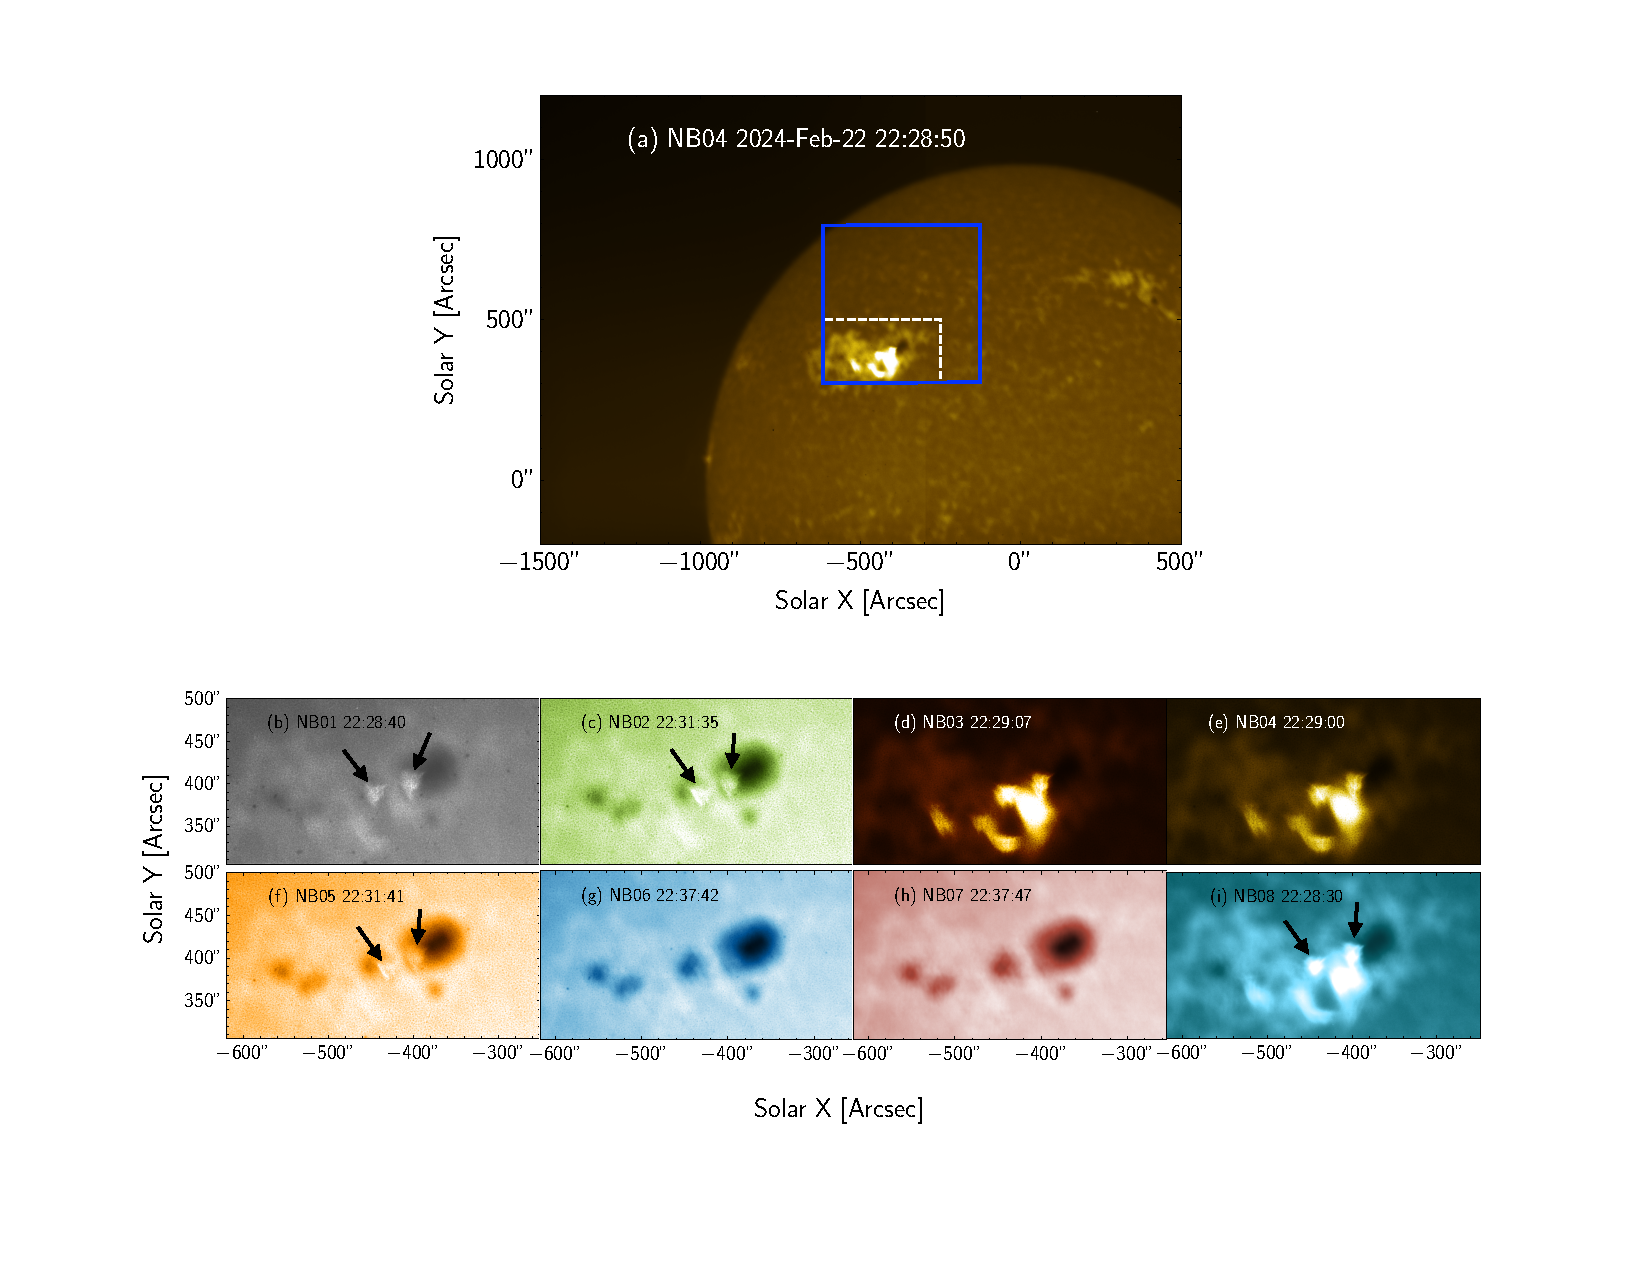
\includegraphics[trim = {2cm 2.5cm 2cm 1.8cm}, clip, width=0.9\textwidth]{Figures/feb_22nd/suit_roi_all_peak.pdf} 
    \caption[SUIT observation of the flare in all NB filters at their respective peaks]{(a) Parts of the full-disk (2k$\times$2k) observation in NB4 (\ion{Mg}{2}~h) showing the flaring region and sunspot. The over-plotted blue box shows the RoI localized by the onboard flare detection algorithm, and the white dashed box locates the region used for the subsequent analysis. (b) SUIT Narrowband images recorded at the peak of flares in the respective filters. The size of the images corresponds to the white-boxed region shown in panel a. The arrows mark the two bright umbral kernels.}
    \label{fig:flare_obs}
\end{figure*}
%-----------------------------------------------

\newpage

%-----------------------------------------------
\section{Data Analysis and results}\label{res}
%-----------------------------------------------

%-----------------------------------------------
%\begin{figure}
\begin{wrapfigure}{l}{0.5\textwidth}
    \centering
    \hspace{-1cm}
   \includegraphics[trim={1.5cm 2.5cm 1.5cm 1cm},clip,width=\linewidth]{Figures/feb_22nd/suit_roi_aia_peak.pdf}
    \caption[AIA and GONG observations of the flare]{Co-aligned and co-registered AIA 1600, 1700~{\AA} and GONG H{$\alpha$} observation near the NB3 peak in a, b and c, respectively. The over-plotted contours show 60\% of the peak intensity observed in NB3.}\label{aia}
\end{wrapfigure}
%\end{figure}
%-----------------------------------------------

Figure~\ref{fig:flare_obs}.a displays shows a cutout of the full-disk (2k$\times$2k) image taken in NB4 (\ion{Mg}{2}~h) filter. The over-plotted blue box shows the region of interest automatically defined by the onboard flare detection algorithm. As we can see, the auto-defined RoI fully covers the flare. The flare detection algorithm is designed to define the RoI, which is centred on the flaring region. In the current observation, we can see that the RoI is not properly centred at the flare. However, since then, various parameters of the flare detection and localization algorithm have been tweaked to achieve better detection and localization. The white dashed box locates the region we have considered for further study in this {\bf chapter}. Fig.~\ref{fig:flare_obs}.{b-i} displays the flares in each narrow band filter at their respective peak. The field of view (FOV) corresponds to the dashed white box in panel a. As can be seen, the flare is observed in all the narrow band filters of SUIT, including the two flare kernels observed as penumbral brightening, which are located by black arrows. % in d during the respective peaks of NB2 and NB5 (marked by black arrows in Fig.~\ref{fig:flare_obs}c and f respectively).
%-----------------------------------------------
\begin{figure*}
    \centering
    \includegraphics[trim={0.2cm 2.5cm 1cm 3.5cm},clip,width=\linewidth]{Figures/feb_22nd/suit_roi_nb3_peak.pdf}
    \caption[SUIT observation of the flare in all NB filters at NB3 peak]{Flare as observed in all narrow band filters at the time of peak intensity in NB3. The over-plotted black contours show 60\% of the peak intensity observed in NB3.}
    \label{fig:flare_nb3_peak}
\end{figure*}
%-----------------------------------------------

In Fig.~\ref{fig:flare_nb3_peak}, we plot the flare as observed in each narrow band filter at the peak intensity in NB3(\ion{Mg}{2}~k).%channel at around $\sim$ 22:28-22:29 UT. 
The over-plotted black contours represent 60\% of the peak intensity observed in NB3. The features observed in NB8 (\ion{Ca}{2}~h) are very similar in morphology to those in NB3 and NB4. While there appears to be a hint of such features in other continuum channels, it is not clearly discernible. 

%-----------------------------------------------
\begin{figure*}
    \centering
    \includegraphics[width=0.9\textwidth,trim={1cm 2cm 1cm 4.2cm},clip]{Figures/feb_22nd/lc_4.pdf}
    \caption[Comparison of SUIT NB lightcurve with other observatories]{Light curves obtained over the contoured region from AIA 1600 (blue dashed), AIA 1700~{\AA} (black do-dashed), NB3 (black dotted), NB4 (green dot-dashed), NB8 (magenta dashed), NB2 (blue dotted), NB5 (green dashed), NB1 (green triangles), NB6 (magenta squares) and NB7 (blue dotted) as labelled. For comparison, we have also over-plotted the light curves obtained from coaligned GONG H-alpha observations (blue squares) in panel (a), full-sun integrated GOES/SXR in 1{--}8~{\AA} (red solid) and STIX/HRX (black dashed) in panel (c).}
    \label{fig:flare_lc_suit}
\end{figure*}
%----------------------------------------------- 

To compare the SUIT observations with those from AIA and H$\alpha$, in Fig.~\ref{aia}, we plot display AIA~1600 (panel a), AIA~1700 (panel b) and GONG-H$\alpha$ recorded at near simultaneous time to the peak of NB3 observations. The over-plotted contours are the same as those in Fig~\ref{fig:flare_nb3_peak}. These images clearly reveal the presence of clear signatures of the flare kernels in AIA UV and H$\alpha$ observations, co-spatial to the NB3 (\ion{Mg}{2}~k) observations.

In order to understand the temporal evolution of the flare, we plot the lightcurves in Fig.~\ref{fig:flare_lc_suit} obtained from various filters of SUIT, GOES, STIX, AIA 1600 \& 1700, and GONG H$\alpha$, as labelled. Note that the GOES and STIX lightcurves are full Sun integrated, whereas those for other observations are obtained over the contoured region Figs.~\ref{fig:flare_nb3_peak}~\&~\ref{aia}, and normalized to their respective max intensities. The vertical dotted black line across all the panels locates the peak intensity in NB3. 

The lightcurves reveal that the flare peaks in all the SUIT channels (except NB6 and NB7), AIA 1600 \& 1700, H$\alpha$ and STIX before it achieves its maximum intensity in GOES. The STIX peak coincides with that in SUIT NB1, NB3, NB4, NB8 as well as AIA and H$\alpha$. Note that SUIT NB3, NB4 and NB8 primarily observe the chromospheric signatures, similar to GONG H$\alpha$. Fig.~\ref{fig:flare_lc_suit}.b, shows that the lightcurves of NB3, NB4, and NB8 peak at the same time around $\sim$ 22:29~UT, which is similar to that H$\alpha$. However, NB8 and {\it GONG}-H$\alpha$ show less contrast variation ($\sim$ 40\% change for NB8 (\ion{Ca}{2} h) and GONG H$\alpha$, compared to the $\sim$ 80\% change for NB3 (\ion{Mg}{2} k) and NB4 (\ion{Mg}{2} h)) than that shown by NB3 and NB4. This may be attributed to the larger enhancement in the continuum in NB8 (\ion{Ca}{2}) and H$\alpha$ than that in \ion{Mg}{2}.

Figure~\ref{fig:flare_lc_suit}.c shows that the lightcurves of SUIT NB2 and NB5 (blue and red wing of \ion{Mg}{2}) peak about 3 minutes after the NB3 peak (also STIX hard X-ray peak). This is also apparent in the images shown in Fig~\ref{fig:flare_obs}. Moreover, unlike other lightcurves, NB6 and NB7 lightcurves do not show a gradual increase and decrease. Instead, they exhibit a rather sharp rise, albeit very small ($\sim$ 0.03\%), in intensity during the impulsive phase of the flare.

%%--------------------------------------------
\section{Summary and Discussion}\label{sec:disc}
%%--------------------------------------------

In this {\bf chapter}, we have performed a multi-wavelength study of the X-6.3 flare observed on Feb 22, 2024, using the observations recorded by SUIT, AIA, STIX and GONG. Moreover, this is the first flare detected and localized by the onboard algorithm for flare identification on SUIT and observed in flare mode. Below we summarize the obtained results.
\begin{itemize}
    \item The flare is observed in all narrow band filters of SUIT. The flare was also observed in AIA 1700 and 1600, GONG~H$\alpha$, GOES soft X-rays (SXR) and STIX hard X-rays (HXR).
    \item The flare peak in all SUIT channels (except NB6 and NB7) and those in AIA 1600 \& 1700~{\AA}, GONG~H$\alpha$ and STIX HXR observations and is $\sim$ 5 minutes prior to the GOES SXR peak. The flare peaks are observed in NB6 and NB7 after $\sim$ 3 minutes after the GOES SXR peak.
    \item The flare peak in NB3 and NB4 coincides with that in AIA 1600 \& 1700~{\AA} and STIX 25{--}50~keV observations.
    \item The flare attains its peak in NB2 and NB5, blue and red wing of \ion{Mg}{2} lines, after about 3 minutes it does in NB3.    
\end{itemize}

The results demonstrate that the flare signatures detected by SUIT in all its narrow band channels are very tightly related to HXR observations recorded by STIX. These results highlight the first {\suit} observations of an X-class flare. The observations of flare kernels and enhancement in the intensity in the red wing of the \ion{Mg}{2} window, i.e., NB5 is similar to those observed by \cite{kowalski19,kowalski17,kleint17} using the observations recorded by the Interface Region Imaging Spectrometer \citep[IRIS,][]{iris}. For the flare studied here, we also detect the bright kernels and intensity enhancements in the blue wing of the Mg window, i.e., in NB2 filter. To the best of our knowledge, this is the first such observation in the blue wing of \ion{Mg}{2}. Unfortunately, we can not comment on the spectral nature of the bright kernels as SUIT is only an imager. Further exploration is necessary to comment on the spectral nature of the bright kernels and their possible origin. It is important to highlight that in the observation reported by \cite{kowalski19}, the appearance of flare kernel and intensity enhancement in SJI recorded at 2832~{\AA} (similar to SUIT NB5 filter) corresponded with a plethora of photospheric absorption lines, mostly \ion{Fe}{2}, turning into emission, which was attributed to photospheric heating.  would  Therefore, no such analysis was possible. 
\clearpage
%
%
\chapter{Echoes of the Solar Inferno: Summary and Future Prospects}\label{c:chap8}
\chaptermark{Summary \& Outlook}
\justifying
%XXXXXThis thesis addressed several questions regarding solar flares and their effects on the local plasma environment. We first estimate thermal energies in two solar flares. We use DEM analysis with AIA, XRT and SUVI data to estimate the thermal energy of these flares as a function of time. We describe a method to use stereoscopic observations from AIA and {\it STEREO-A} data to accurately determine the flare arcade volume as a function of time. We also describe multiple initial preparatory analyses we carried out for the design and calibration for {\suit}. We first describe the analysis we carried out with the simulated spacecraft jitter data provided by the ISRO URSC team to quantify the RMS jitter as a function of exposure time. Following this, we describe the throughput model of {\suit} and describe how this method was used to choose the science filters to be mounted on {\suit}. Subsequently, we describe the on-orbit stellar calibration plan of {\suit} using Sirius-A as a calibration source, which is yet to be carried out. We then describe the forward model pipeline we set up to create mock {\suit} observations to characterize the imaging performance and the effects of the instrument PSF on the imaging. Following this, we use IRIS \ion{Mg}{2} data to investigate the effects of Solar flares on the local plasma environment. We describe how similar observations can be used to regularly monitor the similar effects from {\suit} NB3 and NB4 observations. Finally, we describe two of the first flares observed by {\suit}. The main results of this thesis can be summarised as follows:

%\textbf{For the above paragraph -- just compress the three paragraph in the synopsis into one. Then say that we summarise the finding in this thesis below.}

%The below items has to be like abstract for each chapter... 

Solar flares are the most powerful magnetic events in the solar system, characterized by sudden, localized brightening in the solar atmosphere. %These eruptions are triggered by magnetic reconnection, releasing vast amounts of energy in the form of radiation and energetic particles. Solar flares often produce large-scale disturbances, including filament or prominence eruptions, coronal mass ejections (CMEs), and wave phenomena such as Moreton waves and EUV waves. 
The energy released during a flare can affect space weather and disrupt systems such as satellite communications, GPS, power grids, etc., including serious risks to astronauts and spacecraft in orbit. Studying the underlying physics of solar flares helps us better predict these events and mitigate their impacts, which is critical for the safety of both space-based infrastructure and terrestrial technology. %Furthermore, solar flares offer a unique opportunity to study plasma physics processes, such as magnetic reconnection, which are central to solar physics, astrophysics, and even fusion research. 
The extensive observations of flares, especially in soft X-ray, hard X-ray, and EUV wavelengths, we have developed a tremendous understanding of the physical processes at work in flares. However, numerous important questions about the origin and evolution of thermal and non-thermal energies in solar flares, their spectral distribution, and the precise mechanisms behind flare initiation remain. 

The primary aim of this thesis is to perform a multi-wavelength study of solar flares using existing observations and also contribute towards the development of the new observing facility, the Solar Ultraviolet Imaging Telescope (SUIT) onboard Aditya-L1 that provides crucial data for flare studies. The thesis is structured in two parts. In the first part, we address some of these questions by analyzing the temporal evolution of thermal and non-thermal energies in solar flares using EUV and X-ray data from multiple vantage points. In the second part, we conduct preparatory studies for SUIT that include modeling the instrument's performance, assessing spacecraft jitter profiles, establishing calibration methods using stellar observations, and forward modeling of mock SUIT observations. Below, we provide a detailed summary of the work and results that were obtained. %  In preparation for SUIT operations, we also analyze spectral observations in the near-ultraviolet range and initial flare observations, setting a foundation for future flare studies with SUIT. Finally, we highlight and discuss some of the first flare observations carried out with {\suit} and its implications on our understanding of solar flares. The main results of this thesis can be summarized as follows:

%%%%%%%%%%%%%%%%%%%%%%%%%%%%
\begin{enumerate}

    \item The partition between the thermal and the non-thermal energies in solar flares informs us about the relevant physical process taking place during the evolution of the flare. As discussed in \S\ref{sol_flr_energ}, several statistical studies of solar flare energetics \cite[e.g.,][]{warmuth16a, warmuth16b, stosire07, emslie12, inglis14, ash17} have reported on the partition between the thermal and non-thermal energies of the flares. It can be inferred that for bigger flares (e.g., M and X class), there is enough non-thermal energy in electrons to power the thermal radiation. In comparison, there seems to be a deficit in the non-thermal component for the smaller flares. This prompted speculation about a third energy source that could account for the deficit of energy needed to power the thermal component in smaller flares. One of the key similarities of all of these studies was the use of peak thermal energy as the representative of the total thermal energy of the flares. While that is a fair representation of the overall thermal energy budget of an event, it can miss several intricacies throughout the evolution of the flare. In this thesis, we study two flares, one on disk and the other off-limb. We use AIA and XRT observations to compute DEMs and infer the thermal properties of the flaring plasma. We use observations from AIA and EUVI, from a different vantage,  to triangulate the LoS through the flaring plasma. We find that the thermal energy estimation for solar flares can be significantly affected by the volume estimates of the flaring plasma in the impulsive phase. For the November 29, 2020, limb event, we also demonstrated directly from the calculated thermal energy that the cooling pattern of fans is different than the post-flare loops, thereby indicating a possibly different heating mechanism. A hint of such observations has already been alluded to in various existing studies \citep[e.g.,][]{xie23,reeves19,longcope11}. 

    \item Estimating the imaging performance of {\suit} was one of the priorities to characterize and quantify the possible science cases. To this end, we designed a pipeline to create mock {\suit} observations using simulated MURaM cubes. We incorporated lab-measured PSF in the pipeline to create realistic mock observations.  The measured PSF across various channels show $\sim~2\arcsec$ radius of 80\% FWHM for the PSF. This illustrates that the imaging from {\suit} would be able to resolve features $\sim~2\arcsec$ apart with reliable photometric accuracy. 

    \item The intensity ratios of the \ion{Mg}{2}~k~and~h lines can be used to probe the characteristics of the plasma in the {\bf lower} solar atmosphere {\bf in chromosphere and transition region heights}. To obtain the plasma characteristics in flaring regions, we study the variation of \ion{Mg}{2}~k~and~h intensity ratio for three areas belonging to X-class, M-class, and C-class throughout their evolution. For this purpose, we used existing IRIS observations combined with those from AIA, HMI and GOES X-ray light curves. We co-aligned IRIS 2796~{\AA} observations with those from HMI and obtained artificially rastered magnetic field maps corresponding to IRIS maps. This gives us the measure of the photospheric magnetic field for every pixel of the IRIS rasters. We use a double Gaussian function with a symmetric background about the line core to fit the \ion{Mg}{2} k and h lines. In scenarios where the Mg triplet lines are in emission, they are fitted with separate Gaussian functions. We find that the intensity ratios show significant changes during flares, i.e., it peaks minutes before the GOES SXR peak and falls even below the pre-flare level during the peak and decline phase of the flare. A comparison with photospheric magnetic flux density suggests that the change in ratio is independent of flux density. Given that the \ion{Mg}{2} k to h line intensity ratio is representative of the opacity of the local plasma environment, these results are important in the light of heating and cooling of localized plasma and provide further constraint on the understanding of flare physics.

    \item The several flares observed via {\suit} give us a new perspective on observing various eruptions and how they interact with the local plasma environment.  Here, we report the observation of the first flare X6.3 flare SOL2024-02-22T22:08:00 that was localized and observed with the eight narrow band (NB) filters of SUIT. We have also used the co-spatiotemporal observations from SDO/AIA, SolO/STIX and Global Oscillation Network Group (GONG) H$\alpha$ and GOES. We align and co-register SUIT observations with those from AIA 1600, 1700~{\AA} and GONG H$\alpha$ observations and construct light curves from the same regions on them. We compare these light curves with the full-disk integrated GOES SXR and STIX HXR (25{--}50~keV) light curves. We find that all of the SUIT NB1, NB3, NB4, NB8 filters peak simultaneously with HXR and 1600, 1700~{\AA}. In contrast, the NB3 and NB5 lines peak $\sim$~3 minutes later than the HXR peak. The flare peaks in NB6 and NB7 $\sim$~3 mintes after the GOES soft X-ray peak. To the best of our knowledge, this is the first observation of flare in these wavelengths (except in NB3, NB4 and NB5). Moreover, for the first time, we show the presence of bright kernel NB2. These results demonstrate the capabilities of SUIT observations in flare studies.  
    
\end{enumerate}  
%%%%%%%%%%%%%%%%%%%%%%%%%%%%

The results obtained in this thesis help us understand various puzzles of solar flares and provide a number of constraints on the modeling. Additionally, they open up several pathways to further explore the physics of flares. The observations from the SUIT instrument open up a new window for studying solar flares. Below we describe a few projects that naturally arise based on this study. 

%%%%%%%%%%%
\begin{itemize}[label=\ding{226}]

\item Our results in Chap.~\ref{c:chap3} emphasize the critical role of accurate volume estimation in determining the thermal energy of solar flares. Discrepancies in volume estimation, particularly during the impulsive phase and thermal peak, may lead to overestimation of thermal energy because rapid changes in plasma volume occur during these stages. Therefore, we plan to automate the triangulation method to determine the LoS from earth vantage using observations from various instruments and conduct rigorous statistical studies across different flare classes to understand how volume estimation impacts thermal energy calculations. 

%This, in turn, requires high-resolution imaging of the flaring plasma from various vantages to harness the stereoscopic method discussed in chap.~\ref{c:chap3}. While our method is described for EUV observations, a similar method in SXR has been outlined by \cite{ryan24}, using \textit{Hinode}/XRT and \textit{SO}/STIX observations from different vantages to study the 3D evolution of the thermal loop-top source for an M3.9 flare. Currently, this is only feasible in EUV with \textit{STEREO-A}/EUI and \textit{SO}/EUI.
         %\end{enumerate}
        
\item As alluded to in Chap.~\ref{c:chap6}, we did not observe the correlated change in line intensity rations for the X-class flare. It is possible that the change was not observed for the X class flare, simply due to the cadence limitations of IRIS raster scan, along with which regions of the flare arcade are being scanned by IRIS because it is well known that the \ion{Mg}{2} profiles vary significantly in shape and spatially within the flaring region \citep{panos18,dalda23}. The other and more interesting possibility is that in some of the events, depending on their "impulsiveness", there might be different degrees of ionization at play in the chromosphere. This may also indicate a different energy release mechanism during the pre-flare and impulsive phases of the flare.

\item {\suit} provides the first full-disk solar imaging in 11 filters in the wavelength range of 200{--}400~nm. There are previous flare observations in some of the imaging channels {\it, e.g.} NB3, NB4 and NB5 from {\it IRIS} and NB8 from {\it Hinode}/SOT, only in smaller spatial windows. %Therefore, SUIT observations open up a new window for flare studies. One of the key disadvantages of smaller spatial windows is the possibility of missing events due to different pointing. {\suit}, equipped with its flare detection algorithm, has already observed several flares, including various limb events. This provides us our first observation of off-limb flares in all these lines. A larger statistical study with such observations combined with EUV, SXR, HXR, H$\alpha$, and WL observations can provide a more complete picture of how flare energy is deposited across various layers of the solar atmosphere. We specifically want to explore the observation of the probable flare lines observed in the blue wing of \ion{Mg}{2} discussed in chap.~\ref{c:chap7}. We plan to use flare simulations, together with observations from IRIS and XSM when available to comment on the spectral nature and origin of the penumbral bright flare kernels.
        
    \end{itemize}
%%%%%%%%%%%



\clearpage
%
\appendix
\chapter{Calculation of Oscillator strengths for the Mg~\Romannum{2}~k~\&~h lines}\label{c:a1}
\chaptermark{Oscilator Strength Calculation}
%%%%%%%%%%%%
%\renewcommand{\thesection}{6A}
%\section{Calculation of Oscillator strengths for the \ion{Mg}{2}~k~\&~h lines}\label{sec:a1}
%%%%%%%%%%%%


{\bf For a transition from u$\rightarrow$l the oscillator strengths can be expressed as:

%%-----------%%
\begin{equation*}
    f_{lu}~=~\lambda_{lu}^{2}\times \frac{g_{u}}{g_{l}}\times C_{1}\times A_{ul}
\end{equation*}
%%-----------%%
Where, $\mathrm{\lambda_{lu}}$ is the transition wavelength, $\mathrm{g_{u}}$ and $\mathrm{g_{l}}$ are the degeneracy of the upper and lower level and $\mathrm{A_{ul}}$ is the Einstein coefficient for spontaneous emission. Since the \ion{Mg}{2}~k~and~h line transitions happen to same lower energy state from two upper energy states of slightly different energy, this gives us:

%%-----------%%
\begin{equation}\label{eq6.2}
    \frac{f_{k}}{f_{h}}~=~\left(\frac{\lambda_{k}}{\lambda_{h}}\right)^{2}\frac{g_{k}A_{k}}{g_{h}A_{h}}
\end{equation}
%%-----------%%
Both the k and h line transitions are dipole transitions. In case of dipole transitions, the Einstein A coefficient can be expressed as:

%%%%%%%%%%
\begin{equation}
    A_{ul}~=~\frac{C_{2}}{\lambda^{3}}|\bra{l}r\ket{u}|^{2}
\end{equation}
%%%%%%%%%%

\noindent where, $\mathrm{\lambda}$ is the transition wavelength, $\mathrm{J_u}$ is the total angular momentum quantum number of the upper state. This gives us from eqn.~\ref{eq6.2},

%%%%%%%%%%
\begin{equation}\label{eqn6.4}
    \frac{f_k}{f_h}~=~\frac{\lambda_{h}g_k}{\lambda_{k}g_h}\frac{|\bra{3p~^{2}P_{\nicefrac{3}{2}}}\vec{r}\ket{3s~^{2}S_{\nicefrac{1}{2}}}|^{2}}{|\bra{3p~^{2}P_{\nicefrac{1}{2}}}\vec{r}\ket{3s~^{2}S_{\nicefrac{1}{2}}}|^{2}}
\end{equation}
%%%%%%%%%%

Now the radial part of the states $3p~^{2}P_{\nicefrac{3}{2}}$ and $3p~^{2}P_{\nicefrac{3}{2}}$ would be same and cancel out. So, the ratio would depend on the angular part of the wavefunctions. The reduced matrix element for electric dipole transitions between fine-structure states is related to the LS-coupled reduced matrix element by the Wigner-Eckhart theorem:

%%%%%%%%%%
\begin{equation}
    \bra{n'l'j'}r^{(1)}\ket{nlj}~=~(-1)^{l'+s+j+1}\sqrt{(2j'+1)(2j+1)}
    \begin{Bmatrix}
    l' & j' & s\\
    j & l & 1
    \end{Bmatrix} \bra{n'l'}r^{(1)}\ket{nl}
\end{equation}
%%%%%%%%%%

\noindent where $\mathrm{r^{(1)}}$ is the radial part of the position vector operator. For \ion{Mg}{2} the relevant quantum numbers are:

%%%%%%%%%%
\begin{itemize}
    \item l~=~0 (S state), l'~=~1 (P state)
    \item s~=~1/2
    \item j~=~1/2, j'~=~1/2 or 3/2
\end{itemize}
%%%%%%%%%%

\noindent Evaluating the 6j symbols we get:

%%%%%%%%%%%%
\begin{itemize}
    \item For j'~=~3/2: 
        $\begin{Bmatrix}
            1 & 3/2 & 1/2\\
            1/2 & 0 & 1
        \end{Bmatrix}$~=~$1/\sqrt{6}$

    \item For j'~=~1/2:
        $\begin{Bmatrix}
            1 & 1/2 & 1/2\\
            1/2 & 0 & 1
        \end{Bmatrix}$~=~$-1/\sqrt{3}$
\end{itemize}
%%%%%%%%%%%%

\noindent This gives us:

%%%%%%%%%%%%
\begin{equation}
    \frac{|\bra{3p~^{2}P_{\nicefrac{3}{2}}}\vec{r}\ket{3s~^{2}S_{\nicefrac{1}{2}}}|^{2}}{|\bra{3p~^{2}P_{\nicefrac{1}{2}}}\vec{r}\ket{3s~^{2}S_{\nicefrac{1}{2}}}|^{2}}~=~\frac{4.\frac{1}{6}}{2.\frac{1}{3}}~=~1
\end{equation}
%%%%%%%%%%%%

Plugging this back into eqn.~\ref{eqn6.4} we get,

%%%%%%%%%%%%
\begin{align*}
    \frac{f_k}{f_h}~=~\frac{\lambda_h}{\lambda_k}\times \frac{g_k}{g_h}~=~\frac{2.\frac{3}{2}+1}{2.\frac{1}{2}+1}~=~\frac{4}{2}~=~2
\end{align*}
%%%%%%%%%%%%
\noindent where $\frac{\lambda_h}{\lambda_k}~\simeq~1$.}


\renewcommand{\thesection}{\thechapter.\arabic{section}}

% \clearpage
% \renewcommand{\thesection}{\arabic{section}} % Back to normal numbering
% \setcounter{section}{0}
\clearpage

\chapter{Modifications of the cold thick target model}\label{c:a2}
\chaptermark{Kappa Distribution Fit}
The regular observations of solar flares in Soft and Hard X-ray points towards the "thick-target" interpretation \citep{brown71} of flare accelerated electron injection into the Chromosphere. \cite{brown_2003} coined the source-integrated density weighted mean electron flux $\langle nVF\rangle(E)~[\mathrm{e^{-}cm^{-2}s^{-1}keV^{-1}}]$. The observed hard X-ray spectrum then can be expresses as

%%%%%%%
\begin{equation}\label{e1}
    I(\epsilon)~=~\frac{I}{4\pi R^{2}}\int_{\epsilon}^{\infty}~Q(\epsilon,E)\langle nVF\rangle(E)dE~\propto~\epsilon^{-\gamma}
\end{equation}
%%%%%%%

\noindent where R is the distance between the observed and the Sun, and $Q(\epsilon,E)$ is the angle-averaged bremsstrahlung cross section. The usual cold thick target model gives the relation between the mean electron flux and the injected electron rate as 

%%%%%%
\begin{equation}\label{e2}
    \langle nVF\rangle(E)~=~\frac{E}{K}\int_{E}^{\infty}\dot{N}(E_{0})dE_{0}
\end{equation}
%%%%%%

\noindent $K~=~2\pi e^{4}ln(\Lambda)$ is the collision parameter, e is the electron charge in esu and $ln(\Lambda)$ is the Coulomb logarithm\citep{spitzer62}. The limitations of the standard "thick-target model" becomes more evident when we try to define the accelerated electron spectrum from eqn.~\ref{e1} and \ref{e2} we get

%%%%%%
\begin{equation}
    \dot{N}(E)~=~\dot{N_{0}}\frac{\delta-1}{E_c}\left (\frac{E}{E_c}\right )^{-\delta}
\end{equation}
%%%%%%

\noindent where $\delta~=~\gamma+1$. Here, $E_c$ is an arbitrary reference energy called the low energy cutoff, to stop the total rate of injected electron, $\dot{N_0}~=~\int_{E_c}^{\infty}~\dot{N}(E_{0})dE_0[s^{-1}]$ from diverging. The associated total power in the electron is given as

%%%%%
\begin{equation}
    P[keV.s^{-1}]~=~\int_{E_c}^{\infty}E_0N(E_0)dE_0~=~\frac{1}{\delta-2}E_c^{2-\delta}[\dot{N(E_c)}E_c^{\delta}]~=~\frac{\delta-1}{\delta-2}E_c\dot{N_0}
\end{equation}
%%%%%

\noindent As a consequence various physical properties become very strongly dependent on the low energy cut off. The low energy cut off results in non-physical discontinuous electron distribution of a Maxwellian and power law electron distribution. There are several different attempts to mitigate the nonphysical divergence of the thick target power law injection of electrons at lower energies. \cite{kontar15, kontar19} assumed a warm-target corona and cold chromosphere and included energy diffusion, transport and thermalization of the injected electrons through a warm layer of plasma on top of the cold target to rewrite eq.~\ref{e2} as

%%%%%
\begin{align}
    \langle nVF\rangle(E)~&=~\frac{E}{2K}e^{-E/k_{B}T}\int_{E_{min}}^{E}\frac{e^{E_0/k_{B}T}}{E_0G(\sqrt{E_0/k_{B}T})}~dE_0~\times \int_{E_0}^{\infty} \dot{N}(E_0)~dE_0 \notag \\
    &\simeq~\Delta EM\sqrt{\frac{8}{\pi m_e}}\frac{E}{(k_B T)^{3/2}}e^{-E/k_B T}~+~\frac{E}{K}\int_{E}^{\infty}~\dot{N}(E_0)~dE_0
\end{align}
%%%%%

\noindent where $\Delta EM$ is the "thermalized emission measure" which is created via the thermalization of the electrons and can be written as

%%%%%%
\begin{equation}
    \Delta EM~\simeq~\frac{\pi}{K}\sqrt{\frac{m_e}{8}}(k_B T)^{2}\frac{\dot{N_0}}{E_{min}^{1/2}}~\mathrm{where}~E_{min}~\simeq~3k_B T\left( \frac{5\lambda}{L} \right)^4
\end{equation}
%%%%%%

\noindent where $\lambda~=~(k_B T)^{2}/2Kn$ is the collisional mean free path of the injected electrons. The half loop length L, temperature T and number density n are the physical parameters associated with the coronal loops, through which the electrons are injected. This is known as the "warm target model". Although this model still features a low energy cutoff to the injected electron spectrum, the cutoff is now not ad hoc, and determined by the collisional parameters of the electrons through the coronal loops which in turn are determined by the physical thermal properties of the coronal loops. While the warm target model attempts to explain the physical significance of the low energy cutoff, the use of a $\kappa$-distribution injection of electrons has also proven to be very promising. The $\kappa$-distribution is regularly used to model the electron spectrum in in-situ observations and magnetic reconnection events in the Earth atmosphere \citep{maksimovic05, imada11}.

Close to the low energy cut off usually it is expected that Langmuir waves will be generated and grow\citep{emslie84, hannah09}. The interaction between the waves and the injected electron would flatten the energy energy distribution around the low energy cut off. To reflect this various studies \citep{kasparova09, bataglia15, effenberger17} have used the Kappa distribution, consisting of a Maxwellian core and smoothly merged power-law tail, along with a prominent thermal component to fit the observed X-ray spectrum. Apart from not requiring an arbitrary low-energy cutoff $E_c$, the kappa distribution can provide crucial information on the finer details of the electron acceleration, including the physical conditions of the chromosphere ({\it e.g.} wave-particle interaction, beam-plasma interaction etc.) responsible for the origin of it. \cite{bian14, arnold21} demonstrated that, in presence of Coulomb collisions and velocity diffusion the stochastic acceleration of electrons during solar flares can result in $\kappa$-distribution. In addition, as the $\kappa$-distribution covers the complete energy spectrum and is well behaved throughout, it can provide information about the electrons at a very low energies, which is not sensitive to exchange instruments but can be observed via diagnostics from EUV observations.

\cite{bian14} derived the $\kappa$-distribution as a result of stochastic acceleration in collisional plasma as 

%%%%%%
\begin{equation}\label{e5}
    f_k(v)~=~\frac{n_k}{\pi^{3/2}v_{te}^{3}\kappa^{3/2}}\frac{\Gamma(\kappa)}{\Gamma(\kappa-\frac{3}{2})}\left(1+\frac{v^{2}}{\kappa v_{te}^{2}}\right)^{-\kappa}
\end{equation}
%%%%%%
\noindent where $\kappa~=~\tau_{acc}/2\tau_{c}$ is the kappa index, the ratio of acceleration and collisional decelerations time scale, $v_{te}$ is the thermal speed ($\frac{1}{2}m_ev_{te}^{2}~=~k_{B}T_{\kappa}$). The injected electron rate spectrum and the velocity distribution of the injected electron is given by, $\dot{N}(E)~dE~=~Avf_{k}(v)~d^{3}v$, where A is the injection area. For an isotropic electron distribution ($d^{3}v~=~4\pi v^{2}dv$), plugging in eqn.~\ref{e5} we get:

%%%%%
\begin{equation}\label{e6}
    \dot{N}(E)~=~A\sqrt{\frac{8}{\pi m_{e}k_{B}T_{\kappa}}}\frac{n_k \Gamma(\kappa)}{\Gamma(\kappa-\frac{3}{2})}\frac{E/k_{B}T_{\kappa}}{(1+E/\kappa k_{B}T_{\kappa})^{\kappa}}
\end{equation}
%%%%%

\noindent where $n_{k}[cm^{-3}]~=~\int f_{k}(v)~d^{3}v$ is the total electron number density. So, the total electron injection rate is given by

%%%%%
\begin{equation}\label{e7}
    \dot{N_{0}}~=~\int_{0}^{\infty}\dot{N}(E)~dE~=~2An_k\sqrt{\frac{2k_{B}T_{\kappa}}{m_e}}\frac{\kappa^{1/2}}{(\kappa-2)B(\kappa-3/2,1/2)}
\end{equation}
%%%%%

\noindent pluggin eqn.~\ref{e7} back into eqn.~\ref{e6} we get,

%%%%
\begin{equation}
    \dot{N}(E)~=~\frac{\dot{N_0}}{k_{B}T_{\kappa}}\frac{(\kappa-1)(\kappa-2)}{\kappa^2}\frac{E/k_{B}T_{\kappa}}{(1+E/\kappa k_{B}T_{\kappa})^{\kappa}}
\end{equation}
%%%%

\noindent the associated total power in the electrons is given by, 

%%%%%%
\begin{equation}
    P~=~\int_0^{\infty}E_{0}N(E_{0})~dE_{0}~=~\frac{2\dot{N_{0}}k_BT_{\kappa}\kappa}{\kappa-3}
\end{equation}
%%%%%%

%%%%%%%%%%
\begin{figure}
    \centering
    \includegraphics[trim={0.3cm 4cm 0.2cm 0.2cm}, clip, width=0.95\linewidth]{Figures/fit_kappa.pdf}
    \caption{Top panel: STIX spectra integrated between 15:27:00{--}15:27:10~UT during impulsive phase, fitted with `\textit{thcik\_warm\_kappa}' (solid yellow), `\textit{vth}' (solid green) and the complete fit function `\textit{vth+thick\_warm\_kappa}' (solid red line). Bottom panel: The residue of the fit of the STIX spectra.}
    \label{fig:fit_kappa}
\end{figure}
%%%%%%%%%%

We fit the STIX spectra in the same time window as shown in Fig.~\ref{fig:stix_an} with a {\it vth+thick\_warm} and {\it vth+thick\_warm\_kappa} model to compare the two models. We show the {\it vth} (solid green) + {\it warm kappa} electron injection model (solid yellow) fit in Fig.~\ref{fig:fit_kappa} top panel. Fig.~\ref{fig:fit_kappa} lower panel shows the normalized residual of the fit. In Tab.~\ref{tab:my_label} we list the relevant fit parameters from the two respective models. We show the inferred electron injection rate as a function of the electron energy for the {\it warm target+ power law-electron} injection (solid blue) and {\it warm target+ $\kappa$-electron} injection (dashed red) in Fig.~\ref{fig:e-injection} from the fit parameters listed in Tab.~\ref{tab:my_label} for the two distinct electron models. The key thing to notice is the very similar behavior of the models at the higher energy end. The power law injection model goes to 0 very abruptly at the lower energy cutoff ($E_c$), while the kappa distributed electrons slowly taper off at the lower energy end, providing a more physical picture of the injected electron spectra.

%%%%%%%%%%%
\begin{table}[ht!]
    \centering
    \resizebox{0.6\textwidth}{!}{%
    \begin{tabular}{||lcc||}
    \hline
        Parameters & {\it vth+thick\_warm\_kappa} & {\it vth+thick\_warm}\\
    \hline
     & &  \\
       EM[$10^{49}~cm^{-3}$] & 0.078 & 0.078\\
        &  &   \\
       $k_{B}T[keV]$ & 1.30 & 1.30\\
        & &  \\
       $\dot{N_0}[10^{35}~e^{-1}.s^{-1}]$ & 1.17 & 1.89\\
        & &  \\
        $\delta$ & NA & 3.21 \\
         & &  \\
        $\kappa$ & 5.42 & NA \\
         & &  \\
         $E_c$ & NA & .76\\
          & &  \\
        $k_{B}T_{\kappa}$ & 2.57 & NA \\
         & & \\
         
    \hline
    \end{tabular}}
    \caption{Comparison of various model parameters between "{\it vth+thick2}", "{\it vth+thick\_warm}" and "{\it vth+thick\_warm\_kappa}" model for the same time window of STIX spectra as shown in Fig.~\ref{fig:stix_an}.}
    \label{tab:my_label}
\end{table}
%%%%%%%%%%%

%%%%%%
\begin{figure}
    \centering
    \includegraphics[width=0.8\linewidth, trim={0cm 0cm 1cm 1cm}, clip]{Figures/e_ij.pdf}
    \caption{Inferred electron injection rate as a function of energy for power law electron injection (solid blue) and $\kappa$-distributed electron injection (dashed red) from the fit parameters listed in Tab.~\ref{tab:my_label}.}
    \label{fig:e-injection}
\end{figure}
%%%%%%
\clearpage

% I changed  thebibliography in hvdthesis.cls, so that it generates
% a ToC entry, and is headed References instead of Bibliography. -SR
\singlespace
%\bibliographystyle{aasjournal}
\bibliography{your_bib_file}

\end{document}
